\documentclass[a4paper]{report}
\usepackage{fancyhdr}
\usepackage[ddmmyyyy,hhmmss]{datetime}
\usepackage{tcolorbox}
\usepackage[numbers,square,sort&compress]{natbib}
\usepackage[
  colorlinks=true,
  breaklinks=true,
  allcolors=blue]{hyperref}
\usepackage{chapterbib}
\usepackage{listings}
\usepackage{graphicx}
\usepackage[colorinlistoftodos]{todonotes}
\usepackage[]{algorithm}
\usepackage{algpseudocode}
\usepackage{amssymb}
\usepackage[caption=false]{subfig}

\def\UrlBreaks{\do\/\do-}

\setcounter{tocdepth}{3}
\setcounter{secnumdepth}{4}

\usepackage[a4paper,top=3cm,bottom=2cm,left=3cm,right=3cm,marginparwidth=1.75cm]{geometry}


\usepackage{listings}
\lstset{float,
  % basicstyle=\scriptsize,
  % language=SQL,
  columns=fullflexible,
  % frame=tb,
  captionpos=b,
  mathescape=true,
  tabsize=2,
  xleftmargin=\parindent,
  escapeinside={(*@}{@*)}}

\pagestyle{fancy}
\lhead{}
\rfoot{Compiled on \today\ at \currenttime}
\cfoot{}
\lfoot{Page \thepage}

\makeindex

\title{A flexible and decentralised approach to query processing for geo-distributed data systems}
\author{Dimitrios Vasilas}
\date{}

\begin{document}

\maketitle

\listoftodos

\tableofcontents

\maketitle

\chapter{Introduction}
\label{ch:intro}
% \section{Background and motivation}

Today's global-scale services handle large volumes of data and serve large volumes of requests from users distributed worldwide.
They rely on large-scale data serving systems which distribute data across multiple geographically distant data centers
in order to reduce response time and tolerate failures.
Moreover, services increasingly spread their data between on-premise and remote cloud nodes,
as well as between multiple cloud providers, in order to increase reliability and reduce costs.

An important aspect of the data systems that developers rely on for building applications is a powerful query language.
Google, describing the evolution of Spanner from a key-value store to a relational database \cite{corbett:spanner},
has reported that Google developers found it difficult to build applications on a system lacking a strong schema system
and a robust query language.
Query processing is an essential component of data systems' technology, as its role is to bridge declarative query languages,
in which queries specify the patterns and conditions that results must meet, and efficient execution.

In this thesis, we study the challenges of supporting efficient query processing in contexts in
which users and data are distributed across multiple geographic locations.
In particular, we examine the design decisions and trade-offs involved in the design of a query engine over geo-distributed
data, which serves users distributed worldwide.
We consider a query engine that implement operators for performing transformations over a corpus (selections, aggregations, joins)
and, in addition, employs techniques for accelerating query processing.
These techniques commonly involve the materialization of \textit{derived state}.
This includes maintaining copies of the data organized in forms that facilitate different access patterns (indexes),
and pre-computing the results of expensive recurring operations (materialized views).

The design of such a query engine must meet multiple requirements.
Applications expect query engines to serve requests in a timely fashion and to provide accurate results.
Moreover, query processing must incur low overhead to other aspects of data systems' operation and to their operational cost.

% It is well known that
Query processing in a geo-distributed context involves several challenges.
In geo-distributed deployments,
latencies between data centers can be orders of magnitude higher that those within a data center.
Moreover, network resources between data centers are often limited and costly.
Because of these factors,
in geo-distributed query processing
the requirements of low response time, accurate query results and low overhead to the system's performance and operational
cost are incompatible and cannot be achieved all at once:
% incompatible and thus query engines must balance trade-offs between desirable properties.

\begin{itemize}
  \item User-perceived query response time is composed of two components:
  query network time, which accounts for the time spent to send a query from the user to the query engine over the network
  and the time spent to send search results back to the user, and query processing time.
  Techniques for reducing query processing time, like the above-mentioned, have been extensively studied in the context of database systems.
  However, in geo-distributed scenarios, query network time becomes a significant factor to query response time.

  \item At the same time, the derived state structures that query engines use to accelerate query processing must be kept up-to-date with changes to the corpus.
  This requires propagating and applying the effects of write operations to the derived state.
  Because of that, maintaining indexes and materialized views incurs overhead to the latency of write operations.
  An approach employed by query engines to address this issue is to perform this maintenance task asynchronously,
  outside of the critical path of write operations.
  This, however, entails that derived state is only eventually consistent, and can be temporarily stale relative to the corpus.
  Serving queries from stale indexes or materialized views may result in query results not being consistent with the state of the corpus.
\end{itemize}

Query network time can be reduced by replicating the query engine's derived state on every data center,
thus ensuring that all queries can be served from the local data center without requiring communication with other data centers.
However, maintaining a full replica of every index and materialized view on every data center incurs significant memory and storage overhead.
Moreover, to remain up-to-date with the corpus, a derived state replica must receive the effects of write operation from every data center.
Assuming asynchronous maintenance, this means that derived state can become significantly stale, affecting the accuracy of query results.
In addition, in write-dominated workloads, this results in significant data transfer between data centers for state maintenance.

At the other end of the design space,
derived state can be partitioned into non-overlapping parts and each part assigned to a data center
This approach improves derived state freshness.
However, every query needs to be forwarded to every part of the derived state, resulting in significant overhead in query network time.
Moreover, in query-dominated workloads this increases data transfer between data centers for query processing.

It becomes apparent that, in this setting, design decisions and about the distribution and placement of derive state
and the communication patterns between the corpus, the users and the derived state,
result in trade-offs between query response time, query result consistency, and the system's operational cost.
Techniques such as caching of query results add additional points in this design space.

At the same time,
modern applications have diverse query processing requirements.
User-facing queries have strict response time requirements, as response times directly affect revenues.
On the other hand, query engines that serve social media applications are required to ingest new content rapidly \cite{busch:earlybird}.

In addition to that, different design decisions about derived state distribution and placement are better suited to different workload characteristics.
A design that requires only local communication between the corpus and derived state is better suited for write-dominated workloads in terms of data transfer costs.
Conversely, a design that requires only local communication for query processing is more cost-effective for query-dominated workloads.

It therefore becomes evident that no single query engine design can be suitable for all needs.
However, existing query engines are designed to be general-purpose systems;
They aim at handling a variety of use cases and workloads.
In the context of geo-distribution, general-purpose query engines are often inefficient for certain workloads
and application requirements.
Specialized solutions can be much more efficient,
but adjusting derived state distribution and placement in current query engine architectures can be time and resource consuming.

In this thesis, we make the case for a \textit{flexible} query engine architecture that can be adjusted to the requirements
and characteristics of different applications in a case-by-case basis, with low engineering effort.

\section{Contributions}

Traditional monolithic query engine architectures do not provide the flexibility required to adjust the trade-offs
between query response time, query result consistency, and operational cost according to the characteristics and
requirements of different geo-distributed applications.

To address this challenge, we propose a new \textit{modular} query engine architecture.
Our key insight is that query processing can be decomposed into a set primitives,
such as selecting from a set of data items the ones that satisfy a given condition,
or constructing from a set of data items a secondary index on a given attribute.
Each primitive can be encapsulated by an independent component that interoperates with other components through a set of interfaces.
We show that, while different components encapsulate different query processing primitives,
all components can expose a common set of interfaces with common semantics.

Guided by this insight,
we introduce an architecture component abstraction, called Query Processing Unit (QPU).
The QPU abstraction defines the properties, interfaces and semantics of a generic query engine component.
In order to express different types of query processing primitives,
the QPU abstraction combines the properties of a streaming operator and a microservice.
Akin to a microservice, a QPU component maintains internal state, is configured independently, and exposes its functionality to other components through a service interface;
Akin to a streaming operator, a QPU component operates by receiving one or more input streams from other components,
performs a computation over these streams, and emits an output stream.

Different instantiations of the QPU abstraction (QPU classes) implement different query processing primitives.
These include relational operators, such as selections, aggregations, and joins,
derived state structures, such as indexes, materialized views and caches,
and ``routing'' functionalities, such as load balancing, and managing index partitions.

Query Processing Units are aimed to be used as building blocks for constructing query engine architectures.
A query engine is a directed acyclic graph (DAG), with QPUs as vertices;
Graph edges indicate communication paths between QPUs.
An edge from $QPU_A$ to $QPU_B$ indicates that $QPU_A$ can invoke the interface of $QPU_B$,
and that, as a result, it can receive an input stream from $QPU_B$.
By specifying the QPU class and configuration of each graph vertex, as well as the graph topology,
one can control how query engine's derived state is partitioned,
and the communication patterns required for query processing and state maintenance.
Because the operation of a QPU depends only on its interaction with other QPUs and not its placement,
each QPU can be strategically placed across the system.

A QPU DAG runs a bidirectional data-flow computation.
The corpus is situated at the leaf nodes of the graph, while queries enter the graph through root nodes.
Updates to the corpus stream ``upwards''
\footnote{upwards and downwards are our representational convention} through the query engine graph, and incrementally update the QPUs’ internal data structures;
Conversely, queries stream ``downwards'', are incrementally transformed in sub-queries which are processed in different parts of the graph.
Partial results are then incrementally combined (flowing back upward) to produce the query response.

\medskip
\noindent
We realize this architecture model in the form of a query processing framework, called Proteus.
Proteus provides a library of Query Processing Unit implementations,
a service discovery mechanism that allows QPU graphs to self-organize with only local configuration to each QPU,
and a configuration language for specifying query engine architectures.

Proteus aims at enabling developers to design and deploy query engines in a case-by-case basis,
by enabling flexibility over the distribution and placement of the query engine's state and computations.

% In its current form, the architectural model is not focused on general purpose query engine that can execute an ad-hoc query.
% instead, a query engine is constructed and deployed with a specific query workload (set of queries) in mind.

In summary, this work makes the following contributions:

\begin{itemize}
  \item A comprehensive analysis of the design choices and corresponding trade-offs of geo-distributed query processing.

  \item A novel modular query engine architectural model, based on the Query Processing Unit abstraction,
  which enables flexible distribution and placement of query processing state and computations.

  \item Case studies that demonstrate how a flexible query engines architectures can be applied to a number of applications
  and provide improvements over state-of-the-art approaches.

  \item Proteus, a framework for constructing and deploying query engines using the proposed architectural model.

  \item An experimental evaluation that confirms the theoretic trade-off analysis,
  by demonstrating the benefits and drawbacks of different and placement schemes,
  and shows that Proteus can efficiently implement different points in the design space of query processing state placement.
\end{itemize}

Contributions of the thesis are presented in \cite{10.1145/3194261.3194265} and \cite{app:rep:sh222}.


\section{Thesis outline}

The rest of this thesis is organized as follows.
Chapter \ref{ch:models} introduces the system and data model that we consider in this work,
and discusses the requirements for an efficient and effective query engine design.
Chapter \ref{ch:background} provides an overview of concepts related to the work presented in this thesis.
It provides a broad overview of query processing in database systems,
focusing on techniques for facilitating query processing by maintaining derived state (indexes, materialized views and caches).
Chapter \ref{ch:design_space} presents an analysis of the design decisions and trade-offs involved in the design
of query engines that derived state.
Chapter \ref{ch:design_pattern} presents the specification of the Query Processing Unit abstraction,
and the proposed query engine architecture model.
Chapter \ref{ch:case_studies} demonstrates the proposed architecture's expressiveness by applying it to a number
of use cases and applications showing how it can provide improvements over the state-of-the-art.
Chapter \ref{ch:proteus} describes the Proteus framework.
Chapter \ref{ch:evaluation} evaluates the proposed approach,
and shows how flexible state and computation placement can allow applications to balance the trade-offs between
query response time, result accuracy and operational cost.
Chapter \ref{ch:related_work} overviews related work.
Chapter \ref{ch:future} outlines directions for future work.
Finally, Chapter \ref{ch:conclusion} concludes the thesis.


% TODO: find a better name
% Data serving systems
\chapter{Background}
\label{ch:background}
% \begin{tcolorbox}
% The goal of this chapter is to prepare the ground so that the reader has the mental framework needed to understand the
% rest of this document.

% This includes:
% \begin{itemize}
%   \item Implicitly establishing a terminology to be used throughout the document.
%   \item Establishing a ''world view'' by describing the system and data model that we consider, and the assumptions that
%   we make
%   \item Establishing concepts that will guide our design decisions in the following chapters (see
%   Section~\ref{sec:requirements}).
%   \item Introducing technical background that will be needed for the following chapters.
% \end{itemize}
% \end{tcolorbox}

\section{Models}
We consider a data serving system with a two-tiered architecture: a data storage tier and a query processing tier.

\begin{itemize}
\item The data storage tier is responsible for providing access to data.
We use the terms \textit{storage system} or \textit{data store} for the system that implement this tier, and the terms
\textit{base data} or \textit{corpus} for its data.
\item The query processing tier is responsible for providing the functionality to identify and retrieve data using
queries on secondary attributes (Section~\ref{subsec:query_prcessing_tier}).

We use the terms \textit{query engine} or \textit{query (processing) system} for the system that implements this tier.
\end{itemize}

Disaggregating query processing from the storage engine is an approach used by various systems and cloud
services such as Amazon Athena \cite{aws:athena}, Aurora \cite{aws:aurora}, and Google BigQuery
\cite{google:bigquery}.
In these systems, query processing is performed by a query engine independent from the storage system.

This model provides several benefits:
\begin{itemize}
  \item Storage and query processing resources can scale independently (elasticity).
  \item It enables on-demand, short-lived queries on already existing data without the need to migrate data.
  \item It enabling cloud providers to implement fine-grained pricing for querying services.
\end{itemize}

In this work, we focus on the design of the query processing tier and consider the data storage tier as ``imposed'':
we consider the data storage tier's functionalities, guarantees, and data distribution schemes as input parameters in
our design.

One of our design goals
(TODO: link to design goals in the next chapter)
is that the query processing tier should be agnostic of the data storage tier.
A query system should be able to interoperate with multiple different data storage tier implementations.
To achieve that, we model the interconnection between tiers as a set of well-defined APIs, which we describe
in detail in the following section.


\subsection{Data storage tier}

TODO: [...] or even streaming systems.

The data storage tier is a broad abstraction that can include any system that can be used to store and retrieve data.
This can include databases, file systems, cloud object storage systems.

As described above, in this work we view this tier as an external, underlying system that our design can build upon.
However, any efficient query processing tier design needs to take into account the properties and characteristics of the
data storage tier, most importantly its data distribution scheme.
To address that, we adopt a less broad data storage tier definition.
More specifically, we model a data storage tier as a federation of geo-replicated storage systems.
In the following Section, we present in detail our data storage tier model.


\subsubsection{System model}
The data storage tier is implemented by a storage system (a database, file system or cloud storage system) or a
federation of multiple, potentially heterogeneous storage systems.
Each system is responsible for storing a dataset $D$.
In a federated system, the dataset of each storage system is independent, but the application logic may implement
replication across different systems (for example an application that replicates data across multiple cloud providers).
In addition, storage systems implement replication:
each storage system maintains one or more full replicas of its dataset, and may also maintain partial replicas.
Finally, replicas are sharded: each replica partitions its data in non-overlapping parts, and a shard is responsible
for a part of the data.

We model the infrastructure on which the data storage tier runs as a collection of \textit{sites}.
A site is a group of nodes (servers, user devices) with the following characteristics:
\begin{itemize}
  \item Network communication latency between nodes in different sites is significantly higher (typically an order of
  magnitude higher) \cite{pbailis:hats} compared to communication latency within a site.
  \item Network resources across sites are more limited and costly across sites.
  This is reflected in the pricing for cross-region data transfer in public cloud platforms.
  Using the AWS Pricing Calculator \cite{aws:costcalc} we see that data transfer to different AWS data centers
  (regions) costs double the price of intra-DC data transfer (0.02 and 0.01 USD per GB respectively).
\end{itemize}

A site can correspond to a data center, a group of servers serving as an edge Point of Presence \cite{google:infra}, or
a group of user devices in close proximity (in the same room or building).


\subsubsection{Data model}

% - Each record also has associated attributes. An attribute is a key-value pair. Schema can be pre-defined or not.
% - Argue that this data model can express a variety of data models (relational, wide-column, object storage). \\
The corpus dataset is a collection of \textit{data items}, organized in \textit{tables}.
We use the term \textit{data item} to refer to the unit of stored data:
Depending on the storage system, a data item may correspond to a file, and object, or a database record.
Tables may be organized in a hierarchical structure (file system repositories), a flat namespace (object store buckets),
or a relational schema.

A data item is composed of a primary key, a set of attributes, and optionally a value.
The primary key can be used to efficiently identify and retrieve the data item, without requiring a scan.
Attributes are key-value pairs: each data item is associated with a map of attribute keys and values
$\{AttrKey: AttrVal\}$.
We do not assume a strict schema for attributes: the attributes of each data item are independent of the attributes of
others.
Finally, we consider the data item's value as a blob of binary data.

We assume that objects are ''versioned``.
Each object is associated with a timestamp, which is one of it's attributes.
A timestamp can be implemented by any data type that provides a comparison operator which can be used to establish an
at least partial order between timestamps, such as Unix time or vector timestamps.

\subsubsection{Data storage tier API}

The data storage tier exposes at least one of the following APIs:
\begin{itemize}
  \item An API for iterating over the corpus data (List)
  \item An API for subscribing to notification for changes to the corpus data.
  \item An API for querying the corpus data.
\end{itemize}

\noindent
\textbf{API 1: List}

\noindent
This API provides a mechanism for retrieving the primary key and attributes of all objects in a given table:

$List(Table, [Timestamp_{low}, Timestamp_{high}))$ $\rightarrow$ $[ListResponse]$

\noindent
Given a table name ($Table$) and a range of timestamps ($[Timestamp_{low}, Timestamp_{high})$),
$ListResponse$ contains all data items in $Table$ with $Timestamp_{low} \leq Timestamp < Timestamp_{high}$.
Each data item in $ListResponse$ is represented as a tuple $(ID, \{AttrKey: AttrVal\})$, containing the data item's
primary key ($ID$), and attributes ($\{AttrKey: AttrVal\}$).

$ListResponse$ may be implemented in different ways, such a single response containing a set of
data items, or a stream in which each data item is sent as a record, or an iterator in which calling a $Next()$ method
returns the following data item.
Finally, We don't assume any ordering in $ListResponse$.

The $List$ API may be provided as an explicit API method or implemented as a combination of a \textit{list} and a
\textit{read} (get) operation.

Depending on its versioning mechanism, the storage system implementing the data storage tier may not support the
listing API for any range of timestamps.
For example, in a storage system that does not provide multi-versioned storage, $List$ will return the latest version of
each data item.
For simplicity, we assume the $List$ API as specified above.
In Section
TODO
we describe how our design can cater for a $List$ API without support for Timestamp ranges.

\noindent
\textbf{API 2: Subscribe}
  for example triggers in traditional
  database management systems, or event notification mechanisms in cloud storage services.

% TODO: cite https://docs.aws.amazon.com/AmazonS3/latest/dev/NotificationHowTo.html


% From the point of view of the query tier, the data storage tier can be models as a system that exposes (one or more of)
% the following APIs:





%  ---
% Each data item is associated with a primary key, $id$, that can be used to efficiently retrieve it, without requiring a scan.
% Data items are associated with a set of attributes, and optionally a value.

% We represent this as a tuple $(V, \{Attr: AttrVal\})$, where $V$ is the data item's value, and $\{Attr: AttrVal\}$ is a map from attributes keys to attribute values.
% Attributes can include system metadata (e.g. size), user-defined tags, or attributes computed from $V$.
% We use the notation $Attr(d)$ to refer to the attribute value of the attribute $Attr$ of data item $d$.

% However, $Attr(d)$ is a partial mapping: some data items may not have a value ($Null$) for $Attr$.

% We assume that every data item has at least one attribute, a ``last-modified'' timestamp, which we describe later in this Section.
% \end{itemize}
% This abstraction is compatible with several different data models, including object storage, document databases, key-value stores, wide-column stores, and relational databases.




% The data storage tier is deployed on
% It fully or partially replicates $D_i$ across different geo-locations, which we refer to as data centers.

% Each data center is partitioned multiple parts, and each partition is responsible for a non-overlapping subset of $D_i$.
% We assume that each database engine instance employs the same partitioning across all data centers, but different instances may employ different partitioning schemes.

% We assume that database engines support three operations: i) a read operation that, given a primary key, returns the value and attributes of the corresponding object, ii) a write operation that updates the value and attributes of a given data item (inserting a new data item can be represented as a write operation), and iii) a delete operation which removes a given data item from $D$.
% The unit of operation on the database engine is the transaction.

% A transaction may contain multiple operations, and is terminated by an abort (writes and deletes have no effect) or a commit (writes and deletes modify the corpus).
% When a transaction commits an update, the database system does not overwrite the data item with the result of the update, but creates a new version instead.
% Each data item version is associated with a version timestamp $vt$, which is one of the data item's attributes.

% We define as \textit{snapshot} a cut of the database's state, a state of data item state containing a version of every data item in the database.
% Each snapshot is identified by a timestamp $ts$.
% The snapshot $ts$ contains the version $vts$ of each data item $d$ in $D$ for which $vts \leq ts$ $\land$ $\nexists$ $vts'$: $vts \leq vts' < ts$.

% We also assume that database engines provide the following mechanisms:


% \textbf{Data (corpus) model} \\
% In short, the corpus is a collection of records grouped in tables. Each record is identified by a unique key (can be a
% composite key).
% Each record also has associated attributes. An attribute is a key-value pair. Schema can be pre-defined or not.

% Argue that this data model can express a variety of data models (relational, wide-column, object storage). \\

% \subsection{Corpus data and system model}
% The corpus is a data set $D$, which is a collection of \textit{data items} with the following properties:
% \begin{itemize}
% \item A data item $d$ in $D$ is associated with a primary key, $id$, that can be used to efficiently retrieve $d$.
% \item A data item $d$ is composed of a value and a collection of attributes.
% We represent this as a tuple $(V, \{Attr: AttrVal\})$, where $V$ is the data item's value, and $\{Attr: AttrVal\}$ is a map from attributes keys to attribute values.
% Attributes can include system metadata (e.g. size), user-defined tags, or attributes computed from $V$.
% We use the notation $Attr(d)$ to refer to the attribute value of the attribute $Attr$ of data item $d$.
% However, $Attr(d)$ is a partial mapping: some data items may not have a value ($Null$) for $Attr$.
% We assume that every data item has at least one attribute, a ``last-modified'' timestamp, which we describe later in this Section.
% \end{itemize}
% This abstraction is compatible with several different data models, including object storage, document databases, key-value stores, wide-column stores, and relational databases.


% Logically, we consider this tier as a component that may expose some of the following APIs:
% \begin{itemize}
%   \item An API for iterating over the corpus data.
%   \item An API for subscribing to notification for changes to the corpus data.
%   \item An API for querying the corpus data.
% \end{itemize}
% This component can be implementing by an actual storage system that stores the corpus data (in that case it might
% provide all three APIs), or by an event stream providing only the subscription API.

% Also:
% \begin{itemize}
%   \item Describe our assumptions on the consistency guarantees of the storage tier.
%   \item State that we consider this tier ''imposed''; we build on top of it.
% \end{itemize}

\subsection{Query processing tier}
\label{subsec:query_prcessing_tier}
The query processing tier is responsible for providing the functionality of attribute-based data retrieval.
In more detail, given a query expressed as a predicate on attributes and a table, the query processing tier is
responsible for providing the primary keys and attributes of all data items in the given table that match the given
predicate.

As query language, we consider a subset of SQL that contains only expressions of the form: \\

\noindent
$SELECT$ $projection$ $FROM$ $Table$ $WHERE$ $predicate$
\noindent
where
\begin{itemize}
  \item $projection$ is the list of attributes to be included in the query response.
  It has the form $AttrKey_1$, $AttrKey_2$, ..., $AttrKey_N$
  \item $predicate$: has the form: \\ $rangePredicate_1$ $AND$ $rangePredicate_2$ AND ... AND $rangePredicate_N$, \\
  where $rangePredicate_i$ an expression of the form $attrVal_{low}$ $\leq$ $attrKey$ $<$ $attrVal_{high}$.
\end{itemize}

Given a query $Q$ represented as ($projection$, $table$, $predicate$)
and a data item $d$ represented as ($table$, $id$, $attributes$), $d$ satisfies $Q$ if:
\begin{itemize}
  \item $Q.table$ = $d.table$: the data item belongs in the table referred by the query.
  \item $\forall$ ($attrVal_{low}$ $\leq$ $attrKey$ $<$ $attrVal_{high}$) $\in$ $Q.predicate$:
  $attrKey$ $\in$ $d.attributes$ and :  $attrVal_{low}$ $\leq$ $attrVal$ $<$ $attrVal_{high}$:
  the data item contains all attributes included in the query's predicate.
  \item $\forall$
\end{itemize}


% The query subsystem provides the functionality of attribute-based queries.

% A query is defined as a set of tuples $Q = \{(Attr, [AttrVal_1, AttrVal_2))\}$ such that $AttrVal_1 \leq AttrVal_2$.

% We refer to each tuple in a query as a predicate.

% A data item $d$ satisfies $Q$ if $\forall$ $(Attr, [AttrVal_1, AttrVal_2))$ $\in$ $Q$: $Attr(d)$ $\neq$ $Null$ $\land$ $AttrVal_1 \leq Attr(d) < AttrVal_2$.

% Each query contains a predicate on the version timestamp attribute.
% Assuming a predicate $(vt, [t_1, t_2))$, we distinguish the following query semantics:
% \begin{itemize}
% \item \textbf{Snapshot queries.} If $t_1 = t_2 = t$, then the query is executed against the snapshot of $D$ with timestamp $vt \leq t$ $\land$ $\nexists$ $vt'$: $vt \leq vt' < t$.
% \item \textbf{Persistent queries.} if $t_2 >$ $vt_{latest}$, where $vt_{latest}$ is the version timestamp created by the last committed transaction, the query is executed against each new data item version $vt$ created by each transaction commit, while $vt < t_2$.
% \end{itemize}

% We define the set of all data items in $D$ that satisfy a query $Q$ as $Q_r$.
% However, the output $Q_o$ of a query may contain additional data items (false positives), or not contain some of the elements of $Q_r$ (false negatives).
% We define the distance between $Q_o$ and $Q_r$ as query result consistency.


% \begin{itemize}
%   \item Describe the intended functionality.
%   \item Sketch the query language.
% \end{itemize}

Query systems often maintain \textit{derived} state, such as indexes, materialized views or caches, which is
derived from the base data.
Derived state needs to be updated to reflect changes to the base data.
For indexes and materialized views this involves updating their entries according to the base data changes.
For caches this involves invalidating obsolete cache entries.


\subsubsection{Consistency between corpus data and query responses}

\section{Query processing system performance evaluation}
\label{sec:requirements}

The aspects of a query processing system's performance can be categorized in two groups:
\textit{efficiency} and \textit{effectiveness} \cite{buttcher:informationretrieval}.
Efficiency can be measured in terms of time (milliseconds per query) of utilized resources (bytes in memory per based
data record).
Evaluating efficiency involves metrics such as response time, throughput, scalability.
Effectiveness is a measure of how well a query processing system achieves its intended purpose.
Evaluating effectiveness involves measures such as precision and recall.

\subsection{Evaluating Efficiency}

The most visible aspect of efficiency is the \textit{response time} experienced by a user between issuing a query and
receiving the corresponding response.
Since the query system needs to support many simultaneous users, the \textit{query throughput}, measured in queries per
second becomes an important performance factor.
In addition, since response time is the metric that affects user experiences, a performance factor is how
\textit{response time} scales with \textit{query throughput}.
Together, \textit{query throughput} and the relation between \textit{response time} and \textit{query throughput}
characterize the system's \textit{scalability}.

\subsubsection{Response time}
Response time - the amount of between making a request and receiving the corresponding response -
is among important metrics for the quality of user-facing service.

A number of studies and experiments have been studied the effects of response time to user experience.
Results show that response time is among factors that have the largest effect users' subjective perception of the
quality of a system.
Users have been shown to perceive websites that load faster as more interesting \cite{ramsay/retrievaltimesinvestigation}.
On the other hand, long response times increase user frustration \cite{ceaparu:userfrustration} and even compromises
user's conceptions of the security of the system \cite{bouch:qualityeyebeholder}, making users for example less likely to
make purchases on websites with long loading times.

As a result, even small increases in user-perceived response times can result in drops in web traffic and
therefore sales, as industry reports have indicated.
Experiments by the Google and Bing search engines have shown that loner page loading times have a significant impact on
metrics such as time to click, repeat site usage, and queries per visit \cite{schurman:rerformanceuserimpact}.
A study from Akamai on the impact of travel site performance on consumers showed that more than half of the users will
wait three seconds or less before abandon the site \cite{akamai:travelsiteperformance}.
Finally, a comparison shopping service (Shopzilla) has reported that a website re-engineering project that achieved a
speedup in page load time from 6-9 seconds down to 1.2 seconds resulted in 25\% increase in page views and 5-12\%
increase in revenue \cite{dixon:shopzillasiteredo}

\subsection{Evaluating Effectiveness}

Effectiveness is a measure of how well a query processing system achieves its intended purpose.
In the field of information retrieval, the key notion linked effectiveness is \textit{relevance}
\cite{buttcher:informationretrieval}:
Given a user's information need represented by a search query, each document in a given a document collection, is either
relevant or non-relevant with respect to the information need.
The two most used measures in information retrieval systems evaluation are precision and recall.
Recall is the fraction of relevant documents contained in the query result.
It is affected by false-negatives: not including relevant documents in the query result.
Precision is the fraction of relevant documents among the documents contained in the query result.
It is affected by false-positives: including non-relevant documents in the query result.

The difference information retrieval and the query processing model in this work is that here there is no notion of a
ranking function.
In information retrieval relevance is a spectrum: documents can be more or less relevant to a given query.
Here, relevance is binary: a record is either relevant (satisfies the given query) or it is not.


A factor that can affect query effectiveness even when relevance is binary is the consistency between base
and derived data.
In traditional database systems, derived data are kept consistent with base data by being updated in the critical path
of each base data update.
As a result, queries are guaranteed to return all relevant and only relevant results.
However, in systems that implement asynchronous (lazy) derived data maintenance policies \cite{tan:diffindex,
qi:secondaryindexconsistencyanalysis, shukla:schemaagnostic}. derived data can be stale with respect to base data.
This can results in both false-positives and false-negatives.

We use the notion of \textit{freshness} to refer to the measure of inconsistency between base and derived data due to
asynchronous maintenance, which results in lower query processing effectiveness.

TODO: paper about freshness metrics.
% Freshness - Correctness - Consistency

TODO: Availability
TODO: Operational Cost


\subsection{End-user and system operator requirements}

Another categorization of query processing performance aspects can be made between end-user and system operator
requirements.
End-user requirements are performance factors such as response time, effectiveness and availability, which are directly
visible to end-users and affect their experience
System operator requirements such as scalability and cost, which are not directly visible to end-users but are important
for the system's operation.


In this section, present the factors that affect the experience and satisfaction of end-users of the query processing
tier.


% \textbf{Freshness}
% \begin{itemize}
%   \item Define freshness intuitively, as query results being up-to-date with the corpus data.
%   \item Present evidence of use cases in which getting fresh results is important.
% \end{itemize}

% \textbf{Correctness} \\
%   Define correctness using recall and precision.

\textbf{Availability} \\
  Present evidence of the negative effects of downtimes.

% \textbf{Consistency}

% \subsection{System provider requirements}
% In this section, we present factors that are indirectly affect end-users, but are important for the system operator.

\textbf{Scalability} \\
Present evidence of about the scale of internet services nowadays.

\textbf{Operational Cost} \\
The cost of operating the query processing system. Can split to fixed (monthly) cost, and per-query cost.

\bibliographystyle{unsrt}
\bibliography{refs}

\chapter{The design space of geo-distributed query processing}
\label{ch:design_space}
% The goal of this chapter is to draw the design space of designing a query engine.

% Present the different design decisions,
% and the trade-offs the create (how each decision affects the metrics )

% This includes:
% \begin{itemize}
%   \item Listing the axes of the design space, and the options for each axis.
%   \item Describing the expected performance and efficiency characteristics
%   of each point in the design space.
%   \item Describe the trade-offs that occur from the above analysis.
%   \item Discuss the additional challenges/constraints that occur from the geo-
%   distribution of data.
%   \item Present state-of-the-art approaches and their limitations.
% \end{itemize}

% \section{Design choices and trade-offs}
% Describe the design choices involved in design a query engine.
% For each, list the possible options and comment on their effect on the engine's
% performance and efficiency.

% It is well understood that efficient query processing requires tuning on a case-by-case and even query-by-query basis.
% Databases systems allow database administrators to select which indexes to materialize, and choose between different
% index types.
% Relational database systems in particular have a long history of aiming to provide access to data via the use of
% optimizers, components that automatically construct query execution plans, select query operator algorithms etc. based
% on statistics on the characteristics of data.
% The common characteristics of these techniques is that query processing systems are designed as general purpose systems
% and provide mechanisms for optimizing query processing to the characteristics of different use cases \textit{at runtime}.

As discussed in chapter~\ref{ch:background}, secondary indexing, the use of materialized views, and caching are techniques
crucial to providing efficient query processing.
They all involve the use of \textbf{derived state}, specialized representations of the base data that speed up a
particular read access to data.
The use of derived state for efficient query processing involves a number of design decisions.
These decisions are often in tension and create trade-offs.

In this chapter, we describe the design decisions and trade-offs involved in the use of derived state for query processing,
and discuss how difference choices affect the behavior of the query processor.
In addition, we present a framework for reasoning about these design choices and their interactions.

\section{The use of derived state in query processing}

Indexes, materialized views, and caches are all instances of a common technique:
creating derived state by applying a transformation to the data stored in the database in order to speed up a particular
read access to the data.

At an abstract level, derived state can be described by a \textbf{write path} and a \textbf{read path}
\cite{kleppmann:designing}.
The write path is the process of updating the derived state to reflect a change to the base data.
The read path is the process serving a query using the derived state.
% Note that in the case of caches, the read path modifies the derived data (inserting new cache entries after a cache miss).
In other words, the write path is the pre-computation that takes place as soon as a change to the base data occurs,
regardless if the results are going to be consumed by a query;
the read path is the computation that occurs when one reads uses the derived state to process query.

\medskip

We can illustrate how the notion of the read and write path applies on different derived state structures using an example.
Consider a database that stores images.
Each image can be associated with user-defined metadata tags, and the database provides the functionality of
images via queries on those tags.
Consider the query \\

\noindent
$SELECT$ $*$ $FROM$ $photoAlbum$ \\
$WHERE$ $tags.predominantColor$ $BETWEEN$ $\#0a6fb6$ $AND$ $\#52aca2$ \\

\noindent
(this query could for example be part of a service that automatically creates slideshows from the image dataset).

A secondary index on the $predominantColor$ tag can be used to speed up this type of queries.
In that case, the write path updates the index (when images are inserted or deleted), and the read path searches the
index for color values in the range specified by the query, and combines the results.
If an index has not been created, processing the query would involve scanning all the images in $photo-album$:
no work is required in the write path, and significantly more work is needed in the read path.
Using an index, therefore, shifts an amount of computation from the read to the write path.

Another option is to maintain pre-computed search results for the most common queries, so that they can be served
without needing to access the index or scan the dataset.
This can be implemented either as a \textit{cache} of common queries, or as a \textit{materialized view}.
In the case of a cache, the read path either reads from the cache, or falls back to using the index or performing a scan
and then writes to the cache; the write path may invalidate cache entries, depending on the policy that is used.
In the case of a materialized view, the read path read the query results from the view, while the write path updates the
view to reflect updates to the dataset that should be included in the results of the most common queries.

From this example it is clear that indexes, materialized views, and caches can be viewed as techniques for shifting the
boundaries between the read and the write path.
They allow the system to perform more work on the write path, in order to reduce the work needed or speed up the
processing on the read path.
Database systems provide mechanisms for managing this trade-off at runtime, by allowing the database administrator
to select indexes and materialized views to be created, and by providing mechanisms to automate this selection
\cite{valentin:db2advisor, chaudhuri:decadeselftuning}.

\section{Design decisions and trade-offs in derive state based query processing systems}

Designing a query processor that maintains derived state involves a number of design decisions:
\begin{itemize}

  \item Given a change in the base data, when is the derive state updated to reflect this change?

  \item How is the derived state distributed across the system's nodes?

  \item In a system composed of multiple geographically distributed sites, how is the derived state placed across sites?

\end{itemize}

The approaches taken in these questions affect different aspects the query processors characteristics, including query
performance, overhead to write operation, relevance of query results, and operation cost.

These design decisions and their effects to the system's characteristics can be analyzed through the lens of the
read and write path computations to derived data:
\begin{itemize}
  % \item Selecting which indexes and materialize views to create and maintain shifts the \textbf{balance between
  % read-path and write-path computation} (section~ \ref{sec:index_view_selection}).
  % Materializing more views and indexes reduces the amount of work to be done on the read-path, speeding up query
  % processing; it also, however, increases the amount of work on the write-path.
  % This results in a trade-off between the amount of read-path and write-path computation

  \item Selecting between maintaining derived data synchronously or asynchronously, changes the
  \textbf{impact of write-path computation} (section~ \ref{sec:sync_async_maintenance})
  Maintaining derived data synchronously incurs an overhead to write operations, as derived data need to be updated in
  the critical path of writes.
  On the other hand, asynchronous maintenance does not cause an overhead to write operations, but it means that derived
  data are not strongly consistent with the base data.
  Therefore the design decisions on derived state maintenance involve a trade-off between the overhead to write operations
  and the consistency between base and derived data.

  \item In distributed databases, derived data structures are often partitioned,
  and therefore read path and write path computations are distributed computations.
  The partitioning scheme determines the \textbf{communication patterns} of read and write path computations.
  In section~ \ref{sec:index_partitioning} we describe how the choice of index partitioning scheme affects query
  performance and the overhead to write operations (assuming synchronous maintenance).
  The two main index partitioning approaches can be viewed as a trade-off in the volume of communication (number
  of round trips, and number of entities to be contacted) between the read and the write path.

  \item In a database system that is distributed across multiple geographically distributed sites, the placement of
  derived data across sites affects the \textbf{communication latency} of the read-path and write-path computations.
  (section~ \ref{sec:placement})
  Since both clients and base data are distributed across sites, placement decisions involve a trade-off between
  requiring cross-site communication on the read path or the write path.

\end{itemize}

TODO: here we need a visualization for this analysis. a table? a decision tree? both?

It is important to note that the framework of read and write path computations does not include the memory and storage
costs associated with maintaining derived state.

% \subsection{Index and materialized view selection}
% \label{sec:index_view_selection}
% As discussed in chapter~\ref{ch:background} indexes are crucial to query processing performance in most database system.
% The use of indexes provides fast access to data,
% but also complicates updates operations since indexes need to be updated to reflect changes to the indexed data.
% Hence, there is a tradeoff involved in selecting which indices to materialize.
% Having too few or not having the appropriate indexes may force many queries to scan large parts of the dataset;
% Having too many indexes incurs high update costs.

% A similar tradeoff lies in the problem of selecting materialized views.
% Using an appropriate set of materialized views can significantly reduce query response time as processing a query by
% accessing a materialized view can be much faster than processing the query from the base data.
% On the other hand, materializing a view incurs an additional maintenance and storage space cost.

% Therefore, both the index and view selection problem involve a tradeoff between the reduced query response time
% from the one size,
% and write latency and memory/storage space overhead from the other.

% The index and view selection problems have been studied extensively.
% In particular, various commercial and research systems have focused on the problem of automated index selection
% \cite{valentin:db2advisor, chaudhuri:decadeselftuning}

% TODO: methods for finding a rewriting of a query using a set of materialized views -> orthogonal

\subsection{Derive state maintenance policies}
\label{sec:sync_async_maintenance}

Given a database write that updates a data item $d$ by sets the value of an attribute $attr$ $v_1$,
updating derived state (and index or materialized view) that is affected by this update consists of the following steps:
(1) inserting $d$ to the state entries or materialized query results that correspond to $attr$ $=$ $v_1$,
(2) retrieve the value of $attr$ in $d$ before this update, say $v_0$,
(3) and remove $d$ from the state entries or materialized query results that correspond to $attr$ $=$ $v_0$,

The derived state maintenance policy scheme defines when these steps are performed.
In \textbf{synchronous} maintenance, all steps are performed in the critical step of a write operation, usually bundled
as a transaction.
This incurs overhead in write latency, but ensures that derived state is always up-to-date with the base data.

An alternative approach is to perform some of the maintenance step asynchronously: deferring them for after the write
operation has been acknowledged to the client.
This reduces the overhead to write operations, but has the implication that the derived state may be temporarily
stale, representing a previous state of the base data.
If stale derive state is used for query processing, then query results may be inconsistent with the state of the base
dataset, having false-positives and false-negatives.
Therefore, asynchronous state maintenance reduces the query processor's \textit{effectiveness}.

\bigskip

We can view derived state maintenance schemes through the lens of read and write path computation as follows.
The write path computation can be broken down into synchronous and asynchronous computation;
synchronous write path computation incurs an overhead on write operations, while asynchronous write path computation
relaxes the consistency of the derived state.
The state maintenance scheme determines the boundary between synchronous and asynchronous write path computation.
Because reading from inconsistent derived state is possible to results that are not up-to-date with the base data,
maintenance scheme design decisions involve a trade-off between \textit{write overhead} and query result
\textit{effectiveness}.

\bigskip

\noindent
One asynchronous maintenance scheme consists of inserting new derived state entries synchronously (step 2),
and removing the old state entries asynchronously in the background (steps 2 and 3).
The literature often refers to this scheme as \textit{sync-insert}.

The implications of sync-insert is that it reduces the work needed to be done at the critical path of write operations,
but it temporarily leaves stale entries in the derived state, until steps 2 and 3 are performed.
Queries that read from read the stale entries will include false positives in their results.
A common complementary mechanism used with sync-insert is read-repair:
The system validates query results by reading from the base data, and removing false-positive.
Therefore, the read-repair mechanism can be seen as a way to shift an amount of work from the write to the read path.

Another asynchronous policy, termed \textit{async-simple} consists of acknowledging the write operation to the client as
soon as the base data is updated, and performing all derived state maintenance steps in the asynchronously.
In practice, async-simple is implemented using an asynchronous update queue: write operation are acknowledged as soon
as they are logged in the queue; a background process ingests the queue and performs derived state maintenance.

This scheme incurs no overhead to write operations.
However, this approach only provides eventually consistency;
for each write operation there is a time window in which a data item has been updated, but this update has not been
reflected in the derived state.
Reading from the state in this time window, it is possible that a data item that has already been updated in the database
appears with an old value in the query results (neither step 1 nor 3 have been applied), appears to have been remove
from the database (step 3 has been applied, but not step 1), or appears to be associated with two values (step 1 has
been applied but not step 3).

This scheme is used by Amazon's DynamoDB
TODO: cite
% https://docs.aws.amazon.com/amazondynamodb/latest/developerguide/GSI.html
.
Secondary indexes in DynamoDB are update in an eventually consistent fashion.
Because of this applications need to
``anticipate and handle situations where a query on a secondary index returns results that are not up to date''

Diff-Index \cite{tan:diffindex} has proposed an asynchronous index maintenance scheme that provides sessions guarantees.
The technique used to achieve this is to track additional state in the client library:
this state is used to guarantee that any index look-up contains updates to the base data that were made in the same
session.
This guarantees the read-your-writes property.

% So far we have assumed that index updates are synchronous:
% index entries are updated inside the critical path of write operations.
% However, as we discussed in the previous section, in the case of a term-partitioned index,
% index updates are distributed operations.
% This may result in significant overhead to write operations.
% As a result, many databases do not update their indexes synchronously, but rather use asynchronous maintenance schemes.

% -> effect on efficiency : false-positives



\subsection{Index partitioning}
\label{sec:index_partitioning}
Maintaining indexes and materialized views in a distributed database is complex because the partitioning schemes of
derived state do not map to the partitioning of base data, and as a result read path and write path computations may
involve communication among multiple nodes.

The are two main approaches for partitioning an index over a partitioned dataset, presented in chapter~\ref{ch:background},
are:
\begin{itemize}

  \item In \textbf{partitioning by document}, index entries are co-located in the same node as the corresponding
  data items.

  \item In \textbf{partitioning by term}, a global index is partitioned using the same partitioning scheme as the base
  tables, and using the indexes value as the partitioning key.

\end{itemize}

In the partitioning-by-document approach, an index lookup requires broadcasting a read request to every index partition
and then gathering the returned results.
On the other hand, when reading from a term-partitioned index only the index partitions with index entries that are
relevant for the query need to be contacted.
In this approach, however, an additional round of messages is required for retrieving the base data items, as they may
be located on different nodes that the corresponding index entries.
This is not the case for the document-partitioned index, since data items are by-design co-located with the corresponding
index entries.

An advantage of the document-partitioned index is that updating the index upon a write to the database does not require
communication between nodes.
On the other hand, updating a term-partitioned index may involve significant communication overhead, as an update to data
item may involve updating index entries located on different nodes.

\bigskip

These observations can be grouped under the framework of read and write path computations:
partitioning-by-document guarantees local-only communication on the write path, but the most amount of communication on
the write path (a scatter/gather operation involving all index partitions);
partitioning-by-term involves communication across nodes on the write path, but requires less communication on the read
path in the general case (index partitions known do not include relevant index entries are not contacted).

TODO: figures

\bigskip

Guided by this analysis we can reason about the performance characteristics of the two approaches.

Partitioning-by-document is more suitable at a small scale (with a small number of nodes),
while partitioning-by-term becomes preferable as the number of nodes increases and has been shown to provide better
scalability \cite{kejriwal:slik}.

In addition to the system's characteristics, which approach is more suitable for a certain case depends on various
workload characteristics.
In \cite{dsilva:tworings}, D`silva et al. perform an extensive experimental comparison of the two approaches,
implemented in HBase.
Their results show how the performance characteristics of the two approaches is affected by various characteristics of
the workload.

The factors that affect index lookup performance are:
\begin{itemize}

  \item The distribution of values of the indexes attribute:
  As the number of data items per index value increase, the partitioning-by-document approach performs better.
  This is because of the additional round trip required to retrieve the base data items:
  as the number of data items per index value increases, a term-partitioned index is likely to have to contact
  more and more remote nodes, while in a document-partitioned index data items are always co-located on the same node as
  the index entries.

  \item Concurrency:
  As the number of concurrent index lookups increases, the partitioning-by-term approach performs better.
  This can be attributed to the overhead of the scatter/gather operation used by the document-partitioned index:
  As the volume of concurrent index lookups increases, the overhead of broadcasting to every node become more significant.

  \item The selectivity of queries:
  The document-partitioned index outperforms the term-partitioned index as the range of range queries increases.
  This is in accordance with the observation that the partitioning-by-document approach is beneficial where there are
  more records to be returned.

\end{itemize}

In addition, this work assumes synchronous index maintenance, and evaluates the impact of the two approach to write
operations.
The document-partitioned index generally outperforms the term-partitioned for writes, incurring less overhead
and providing better scalability.

From the above analysis it is evident that neither of the two approaches is suitable for all needs.
The choice of which approach to use should be guided by factors including the scale of the system, the properties of the
dataset (distribution of indexed values over the data items), and the characteristics of the workload (query/write ratio,
concurrency, query selectivity):
\begin{itemize}

  \item Document-partitioned indexes are more suitable for: (1) smaller scale systems with a small number of nodes and
  limit concurrency in index lookups, (2) workloads with less selective queries that return large result sets, (3)
  skewed data distribution where a large number of data items have the same indexed value, or (4) write-intensive
  workloads.

  \item Term-partitioned indexes are more suitable for: (1) larger scale systems with a greater number of nodes, (2)
  query-intensive workloads with a large query load, (3) workloads consisting of more selective queries with smaller
  result sets, or (4) data with normal distribution in the indexed value.

\end{itemize}

Clearly, the decision of which index partitioning approach to be used needs be taken in a case-by-case basis.
Database systems should to support both index partitioning schemes, and expose the partitioning scheme selection as a
configuration parameter at the time of creating an index.
We are not aware of any database system that provides this functionality.
In existing systems, this design decision is made at design time, and every index uses the same partitioning scheme.
\cite{}
  TODO: cite.
In Chapter~\ref{ch:case_studies} we demonstrate how a distributed database can provide both index partitioning
schemes.



\subsection{Placement}
\label{sec:placement}



% -> This can apply to any query processing operator, not only stateful ones.

% \subsection{Query processing techniques}

% The choice between
% (1) performing query processing by iterating over the corpus (filtering, aggregation without materialized views)
% (2) maintaining derived state (indexes, materialized views) updated in response to changes to the corpus data
% (3) using caches on top of that.

% \subsubsection{Secondary indexing}

% General system design pattern:
% Having the same data represented in different formats to address different access patterns.

% We have a primary copy of the data in one system (that might be called the source of truth)
% and different derived data systems which they take their data as a copy from this
% primary system.
% Transform it in some way and then represent it differently
% in order to satisfy certain read access patterns.
% Writes go to the primary storage system and all of the other systems are derived from it.
% TODO: address that some systems support writes to a view.
% The other systems only serve read requests.

% \begin{itemize}
%   \item
%   \item it’s just another way of saying we’re going to take the same data and have multiple
%   copies of it represented in different ways, either sorted in a different way, or with a different
%   storage layout.  That allows us to access the data in ways depending on what you’re trying to do. 
%   \item In any relational database, if you have a secondary what you’re really saying is,
%   I want to construct this additional structure on the side (typically a B-tree) and every time you write to some table to update
%   that index to also allow me to find records based on values of a column other than the primary key.
%   (It just happens to be done internally by the database.)
% \end{itemize}

% \subsubsection{Distributed Query planning}

% \subsubsection{Caching}

% \subsection{State maintenance}
% When maintaining derived state, the choice between synchronously versus
% asynchronously updating it for each change to the corpus.

% State maintenance schemes have two characteristics:
% \begin{itemize}
%   \item How much of the state is materialized.
%   When maintaining an index we assume that every index entry is materialized.
%   In contrast, when maintaining a cache, only a subset of entries are
%   materialized
%   (a subtlety here is how an ``entry'' is defined, it might be different between
%   index and cache).
%   There is a finite storage area for materializing entries.
%   When it is filled, some entries are evicted to make space for new entries to
%   be materialized.
%   \item When is the state being updated.
%   The options for this can be:
%   \begin{itemize}
%     \item Update-triggered - Synchronously. When an update to the corpus
%     occurs, it is blocked until the derived state is up-to-date.
%     \item Update-triggered - Asynchronously. Updating the derived state is done
%     outside of the critical path of the corpus update.
%     \item Read-triggered. The derived state mays updated as a response to the
%     state being read (cache misses).
%     This is used in caching.
%   \end{itemize}
% \end{itemize}
%   Based on the above analysis, we can argue that caching is just another state
%   maintenance scheme, and therefore could be treated as a configuration
%   parameter when deploying a QPU.
%   (Note: this is just a way to unify and simplify things by merging caching
%   QPUs with index QPUs, materialized view QPUs etc.)

% \subsection{Component placement}
% There are two types of computational query processing operator can be
% involved in:
% \begin{itemize}
%   \item Update-triggered: For example, updating an index as a result to a corpus
%   update
%   \item Query-triggered: For example, index/cache lookup as a result to a query.
% \end{itemize}
% This can apply to any query processing operator, not only stateful ones.

% The placement determines how close (in terms of network round trip time) the
% operator is placed related to its sources of updates and queries.

% Deciding on placement schemes can lead to trade-offs cause by:
% \begin{itemize}
%   \item The benefits and costs of placing operators close to update sources
%   versus close to query sources.
%   \item An operator might have multiple update and/or query sources.
% \end{itemize}

% We can define ``levels'' of placement: on the same physical machine, on the same
% cluster, in the same DC.

% \section{Trade-offs}
% Summarize how the previously described design choices result to performance and
% efficiency trade-offs.

% Note: This may be redundant depending on how detailed those trade-offs are
% discussed in the previous section, but it is central to the thesis to make the
% argument that it is because of these trade-offs that we propose the QPU
% approach.

% An idea is to here focus on examples of applications that might choose different
% points in these trade-offs.

% \subsection{Response time vs Freshness}

% \subsection{Response time \& Freshness vs Cost}


% \section{Constraints of geo-distributed data}
% Discuss the implication of performing query processing on geo-distributed data,
% and of replicating the derived data used for query processing.

% \subsection{Implications of replicated data in derived state}
% Implication of query processing over AP storage systems:
% \begin{itemize}
%   \item If not carefully designed, concurrent non-conflicting updates may
%   result to conflicts on the derived state.
%   Example: write1: recordX:attributeA=1, write2: recordY:attributeA=1.
%   This results to: index\_update1: add recordX to (attributeA, 1),
%   index\_update2: add recordY to (attributeA, 1).
%   Therefore a ``set CRDT'' behavior is needed for indexes.
%   Generalize to state other than indexes.
%   \item Conflicting updates to the corpus data.
%   Ensure that conflict resolution on corpus data is reflected on derived data.
% \end{itemize}

% \subsection{CAP}
% Describe how query processing performance-availability is constraint by
% CAP in the case of replicated derived state.

\bibliographystyle{plainnat}
\bibliography{refs}

\chapter{A design pattern for configurable query processing architectures}
\label{ch:design_pattern}

We propose a \textit{design pattern} for building query processing systems,
with the goal of evolving query processing system's architecture from monolithic and static to modular and flexible.
Traditional static query processing systems are not able to cater to the needs of modern applications in which users and
data are geo-distributed across the globe.
Our vision is to enable query processing systems that are designed and deployed on a case-by-case basis,
with the workload characteristics, data and access distribution patterns, and requirements of specific applications in
mind.
As a first step towards this vision, we focus on the \textit{mechanisms} required for enabling a flexible and configurable
query processing system architecture.

\medskip

The key idea for the proposed design pattern \textit{assembly-based modularity}.
The query processing system's architecture is modular:
it is constructed by interconnecting composable building blocks
that encapsulate components of a traditional query processing system such as indexes, materialized views,
and caches, as well as relational operators such as filters, aggregations, and joins.
Modularity translates design decisions about the use of derived state to which building blocks are used and how they are
interconnected.
For example, adding a caching layer to an existing system can be done by extending an existing query system architecture
with additional building blocks.

Moreover, modularity enables configurable placement.
The components of a modular architecture, as opposed to a monolithic one,
can be decoupled from the storage tier, and flexibly placed across the system infrastructure.


\section{Overview: a modular query processing architecture}

According to the design pattern that we propose,
a query processing system is a composition of building blocks that encapsulate query processing tasks, called
Query Processing Units (QPUs).

A QPU is a \textit{system component} that combines properties of a microservice and a streaming operator.
Similarly to a streaming operator, a query processing unit receives one or more input streams,
performs a computation over these streams, and emits an output stream.
Similarly to microservice, a QPU exposes an interface for receiving query requests.
The response to query request is a stream.
Moreover, a QPU can send query request to other QPUs.
Therefore, every input stream is the output stream of another QPU, and every output stream is the response to a query request.

\medskip
\noindent
A query processing unit can implement a \textit{relational operator}.
For example, a ``join operator'' QPU receives input streams that represent the tables to be joined,
and emits an output stream that represents the results of the join operation.

Moreover, a QPU can implement a \textit{derived state structure}, such as an index, a materialized view, or a cache.
For example, a ``secondary index'' QPU receives an input stream that represents notifications for updates to the table
to be attribute to be indexed; it maintains a secondary index data structure, which it stores as internal state.
When it receives a query request, it reads from its internal state and emits the result as an output stream.

Finally, multiple ``secondary index'' QPUs can be used to implement partitions of \textit{partitioned index}
Another type of QPU can be then used to as a ``partition manager''; given a query, the ``partition manager'' QPU sends query
requests to the appropriate  ``index partition'' QPUs, thus initiating input streams; it then combines these input streams
and emits the result as an output stream.

Our key insight all three of the described QPU types --- relational operators, derived state, and routing operators ---
can be generalized to a system component with common semantics, and thus can be composed arbitrarily to implement complex
query processing computations.

\medskip
\noindent
QPUs are organized in a directed acyclic graph.
The edges of the graph represent potential query request - response steam relations.
For example, an edge from $QPU_a$ to $QPU_b$ indicates that $QPU_a$ can send query requests (and therefore establish input streams)
to $QPU_b$.
We call $QPU_b$ a \textit{downstream} or \textit{outwards} connection of $QPU_a$.
Base data are the leaves of the graph (nodes with only incoming edges),
and client queries enter the graph through its root nodes (nodes with outgoing edges).

When a QPU receives a query, it can process it by reading from its internal state, it can initiate input streams
by sending query requests to its some of its downstream connections and produce query results using these streams,
or a combination of the two.
This process is recursively performed at each downstream QPU, creating a query execution tree.

\section{Query Processing Unit: the building block}

\subsection{The Query Processing Unit abstraction}

The key property required by query processing unit to effectively serve as building blocks of the modular query
processing systems is composability:
QPUs should be able to be interconnected in various topologies, and interoperate in the execution of query processing tasks.

To achieve this, we define a common set of properties that any query processing unit should conform to.
This properties include a common interface for receiving query request, and common the interaction semantics among QPUs.
We call this set of properties the query processing unit \textit{abstraction}.
Using object-oriented programming terminology, the QPU abstraction can be viewed as an \textit{abstract class}
that defines a set of methods, but does not include their implementation.
Implementations of the QPU abstraction define \textit{QPU classes} with specific functionalities,
such as join or index QPU classes.
Using the object-oriented programming analogy, QPU classes can be viewed as classes that implement the QPU
abstract class.
Finally, specific \textit{QPU instances} can be viewed as objects of a specific QPU class, for example a index QPU that
indexes the attribute $predominantColor$ of a table $photoAlbum$.
The building blocks of a modular query processing system are QPU instances.

In the rest of this thesis we use the terms query processing unit, QPU, and unit interchangeably to refer to QPU instances.

\bigskip

More specifically, the query processing unit abstraction defines a \textit{system component} with the following properties:

\begin{figure}[t]
  \centering
    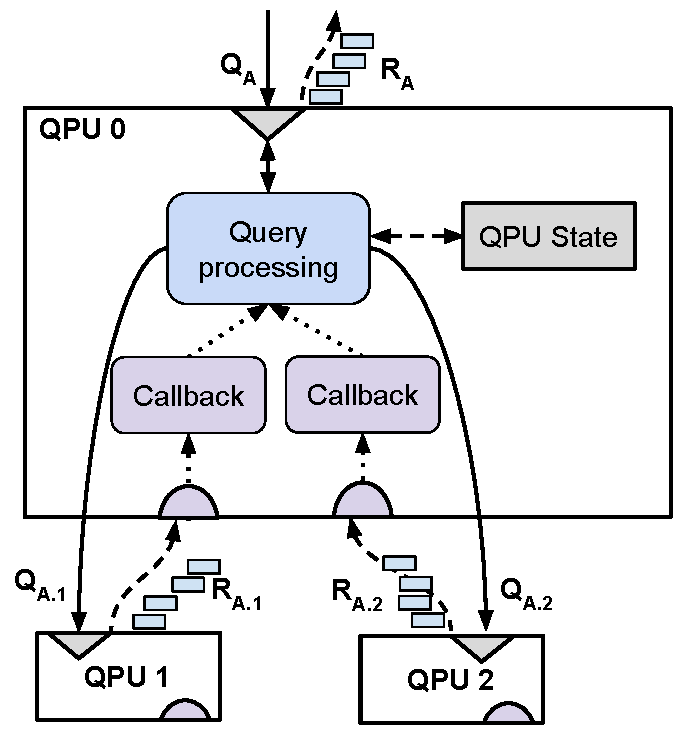
\includegraphics[width=0.5\textwidth]{./figures/design_pattern/qpu_abstraction.pdf}
  \caption{A conceptual depiction the QPU abstraction.}
  \label{fig:qpu_abstraction}
\end{figure}

\medskip
\noindent
\textbf{Query interface.}
Every QPU exposes an interface for receiving query requests.
While this interface is common among all QPUs, QPU classes and specific QPU instances restrict the set of queries
that they can serve.
For example, a QPU may only serve queries about a specific database table.
As a result, QPUs can be though of as microservices that serve queries

The QPU's query interface has \textit{streaming semantics}.
An invocation of the interface establishes between the QPU and caller:
the QPU sends query result entries as stream records; the caller can send control messages such as acknowledgements.
We present the query interface in more detail in section \todo{ref}.

The query interface can be invoked by other query processing units.
This is how QPUs interoperate and forms the basis of the query processing system's computation model \todo{ref}.
We call the act of a $QPU_a$ invoking the query interface of a $QPU_b$, a \textit{downstream query}.

\medskip
\noindent
\textbf{Query processing function.}
Every QPU implements a function that is called when its query interface is invoked, and is responsible for processing
the given query and writing to the query result stream.

The implementation of this computation is specific to each QPU class.

Two capabilities are available for the implementation of the query processing function:
accessing the QPU's state, and initiating input streams by sending query requests to downstream connections.

\medskip
\noindent
\textbf{State.}
Each QPU maintains \textit{internal} state, that is accessible only by that specific QPU.

We distinguish the QPU state in three parts according to its functionality.
In this section, we present an overview of the functionality of each state type.
In section~\ref{ref:specification} we present the QPU's state in detail.

Each query processing unit maintains \textit{configuration state} that represents the query processing unit's
configuration parameters.

In addition, each QPU with outwards connections in the QPU graph maintains information about the
\textit{query processing capabilities} of these QPUs. \todo{ref}.
This information is used by the for creating and generating and sending downstream query requests in order to initiate
input streams that it can use during query processing \todo{ref}.

Finally, query processing units that implement derived state structures, and units need to store intermediate query processing
results, for example \todo{in streaming join computation?}, maintain \textit{query processing state}.

\medskip
\noindent
\textbf{Input stream callback function.}
Each QPU implements a callback function that is called for each record received through an input stream.
Similarly to the query processing function, the implementation to callback function is part of the definition of each
QPU class.

\bigskip

A conceptual depiction of the query processing unit abstraction is shown in Figure~\ref{fig:qpu_abstraction}.
When the QPU's query API is called, a response stream ($R_A$) is established between the unit and the client, and
the unit's query processing computation is invoked.
The query processing computation can read the QPU's state, and can perform downstream queries to other units.
For each downstream query, a corresponding stream is established ($Q_{A.1}$ and $Q_{A.2}$).
When a record is received from one of the streams, the QPU's callback computation is invoked.
Each callback computation processes the received record, and returns the result to the query processing computation.
Upon receiving a result from the callback, the query processing computation can write to the QPU's
state and potentially send a computed query result through the response stream.


\subsection{Query Processing Unit specification}
\label{ref:specification}

In this section we present the detailed specific of the Query Processing Unit abstraction.

\subsubsection{Query interface}

In this section, we first present a high level overview of the QPU abstraction's interface,
and then describe each of its elements in more detail.

Each query processing unit exposes and interface for receiving query requests:


\begin{displaymath}
  Query(QueryRequest) \rightarrow QueryResponse
\end{displaymath}

$QueryRequest$ specifies a predicate on the data items' \textit{attributes}, and a \textit{time interval}.

$QueryResponse$ is a stream containing records that represent \textbf{updates} (an update can be a creation, modification, or deletion)
performed to data item of the corpus
It represents updates as \textit{deltas}:
a delta representing an update $u$ contains the data item's attribute values before $u$ is applied,
and those after the $u$ is applied.

More specifically:
\[
  QueryResponse = [UpdateDelta]
\]
where
\[
  UpdateDelta =
\]
\[
  (DataItemID, [(AttributeName, AttributeValue_{old}, AttributeValue_{new})], timestampValue)
\]
\todo{ensure consistent terminology}

An $update$ is a triplet containing
(1) the primary key of the data item ($DataItemID$) it refers to,
(2) a list of triplets of the form $(AttributeName, AttributeValue_{old}, AttributeValue_{new})$ that represent the
data item's attribute values before and after the update is applied,
and (3) the timestamp ($timestampValue$) assigned to the update.

Given a $QueryRequest$ that specifies an attribute predicate $Pred$ and a time interval $T$ $=$ $[t_1, t_2)$
\begin{itemize}

  \item If $t_1$ $=$ $t_2$ = $t$,
  then for each data item $QueryResponseRecord$ contains \textit{only the latest update before $t$},
  provided that after applying that update the data item's attributes satisfy $Pred$.
  We term this case a \textit{snapshot query}.

  \item if $t_1$ $<$ $t_2$,
  then for each data item $QueryResponseRecord$ contains any update with $t_1$ $\leq$ $timestampValue$ $<$ $t_2$,
  provided that the data item's attributes satisfy $Pred$ \textit{either before or after applied that update}.
  We term this case a \textit{an interval query}.

\end{itemize}

A snapshot query, therefore queries a \textit{snapshot} of the corpus that contains the effect of every update with a
timestamp $<$ $t$.
By returning the latest update before $t$, a snapshot query effectively returns that \textit{state} of the data items
that satisfy $Pred$ in the snapshot defined by $t$.

In contrast, an interval query receives for each data item any update within the specified time interval that modifies
the data item so that either is starts of it stops satisfying $Pred$.
By using a $t_2$ in the future, an interval query can continue receiving updates that satisfy $Pred$.
This provides a mechanism for \textit{subscribing to notification for updates based on a given predicate}.

\bigskip

\textbf{Query Language.}
% https://documentation.basis.com/BASISHelp/WebHelp/usr2/sql_grammar.htm
% http://www.h2database.com/html/grammar.html#expression
% $Query$ receives $QueryRequest$ and returns a stream of $QueryResponseRecord$:

The query processing abstraction implements an SQL-like query language,
that supports point and range queries, logical operators, aggregation functions, and joins.

We argue that these is no inherent limitation in the query processing unit abstraction that prevents it from implementing
more complex functionalities, such as nested queries.
However, we consider additional functionalities to be out of the scope of this work.
We believe this query language can effectively demonstrate that the query processing unit abstraction can be used as building
block for constructing fully-functional query processing systems.

The QPU abstraction's query language has following syntax:

{\obeylines\obeyspaces
\texttt{
QueryRequest          ::=  SELECT SelectExpression
~~~~~~~~~~~~~~~~~~~~~~~~~~~FROM TableExpression
~~~~~~~~~~~~~~~~~~~~~~~~~~~WHERE PredicateExpression
~~~~~~~~~~~~~~~~~~~~~~~~~~~TIMESTAMP TimestampExpression \todo{the timestamp can be just another attribute, but I think we need to have it separate for emphasis}
~~~~~~~~~~~~~~~~~~~~~~~~~~~[ GROUP BY attributeName ]
~~~~~~~~~~~~~~~~~~~~~~~~~~~[ ORDER BY OrderByExpression \{ ASC | DESC \} ]
}}

{\obeylines\obeyspaces
\texttt{
SelectExpression      ::=  ALL
~~~~~~~~~~~~~~~~~~~~~~~~~~~SelectExpressionItem , SelectExpression |
~~~~~~~~~~~~~~~~~~~~~~~~~~~SelectExpressionItem
}}

{\obeylines\obeyspaces
\texttt{
SelectExpressionItem  ::=  SUM(attributeName) | AVG(attributeName) |
~~~~~~~~~~~~~~~~~~~~~~~~~~~MAX(attributeName) | MIN(attributeName) |
~~~~~~~~~~~~~~~~~~~~~~~~~~~attributeName
}}

{\obeylines\obeyspaces
\texttt{
TableExpression       ::=  tableName JoinType tableName USING attributeName |
~~~~~~~~~~~~~~~~~~~~~~~~~~~tableName
}}

{\obeylines\obeyspaces
\texttt{
JoinType              ::=  \{ INNER | \{ LEFT | RIGHT \} OUTER \} JOIN
}}

{\obeylines\obeyspaces
\texttt{
PredicateExpression   ::=  PredicateExpression OR PredicateExpression |
~~~~~~~~~~~~~~~~~~~~~~~~~~~PredicateExpression AND PredicateExpression |
~~~~~~~~~~~~~~~~~~~~~~~~~~~NOT PredicateExpression |
~~~~~~~~~~~~~~~~~~~~~~~~~~~Term Op Term
}}

{\obeylines\obeyspaces
\texttt{
Term                  ::=  attributeName | Value
}}

{\obeylines\obeyspaces
\texttt{
Op                    ::= > | >= | < | <= | = | !=
}}

{\obeylines\obeyspaces
\texttt{
Value                 ::= stringValue | floatValue | intValue |
~~~~~~~~~~~~~~~~~~~~~~~~~~dateTimeValue | timestampValue
}}

{\obeylines\obeyspaces
\texttt{
OrderByExpression     ::= attributeName , OrderByExpression |
~~~~~~~~~~~~~~~~~~~~~~~~~~attributeName
}}

{\obeylines\obeyspaces
\texttt{
TimestampExpression   ::= FROM TimestampTerm [ TO TimestampTerm ]
}}

{\obeylines\obeyspaces
\texttt{
TimestampTerm         ::= SYSTEM START | LATEST | timestampValue
}}

~ \bigskip

In practice, each QPU class can only process a subset of the queries that can be expressed by this query language,
according to its functionality.
For example, a QPU class that implements a join operator can perform a only join over two input streams.
Performing an aggregation or applying a predicate over the result of the join requires this use of other QPU classes.

\todo{references: QPU classes, composition / query execution}

Moreover, individual QPUs of a certain class may support different subsets of the query language according to their
configuration.
For example, two instances of a filter operator QPU class may provide predicate queries for different tables.

% % ---- QPUs are able to send query requests to other units (their child nodes in the QPU graph) by invoking their API.

\subsubsection{QPU State}

A query processing unit maintains the following types of state:

\medskip
\noindent
\textbf{Query processing state}
The QPU's query processing state can be used to implement derived state structures, such as indexes, materialized views and
caches.
In addition it can be use for storing intermediate state used in query processing computations.

We model the query processing state as ordered key/value map, in which keys are string values, and values are lists of
data items, represented as:
\[
  (DataItemID, [(AttributeName, AttributeValue)], timestampValue)
\]

Using pseudocode, we can represent the query processing state as follows:

\begin{lstlisting}[caption={Pseudocode for the QPU's query processing state},captionpos=b,label={lst:qpustate}]
type DataItem {
  dataItemID  string
  attributes  [(AttributeName, AttributeValue)]
  ts          timestamp
}

class QueryProcessingState
  function Get(Key_low, Key_high) [(Key, [DataItem])]
  function Put(Key, [DataItem])
\end{lstlisting}

$Get$ retrieves the query processing state entries with $Key_low$ $<$ $key$ $\leq$ $Key_high$.
$Put$ modifies the value of the query processing state for a given key.
It can be used with a non-existing key to create a new entry, or with an empty value to delete an entry.

\medskip
\noindent
\textbf{Configuration state.}
The configuration state represents the configuration parameters passed to a query processing unit when it is created.

The configuration state consists of two types parameters:
\begin{itemize}
  \item Connection parameters.
  The QPU configuration specifies the endpoints of the unit's downstream connections in the QPU graph.

  \item Class-specific parameters.
  Instances of a QPU class can have different properties.
  For example, different instances a QPU class that implements a query cache can have different cache sizes.
  These characteristics are defined by the QPU's class-specific configuration.

\end{itemize}
% % This is the part of the state that defines the QPU's behavior (includes its type
% % and neighborhood).
% % Passed as argument during initialization.
% % This type of state is composed of configuration parameters, such as the endpoint of its downstream neighbors.

\begin{lstlisting}[caption={Pseudocode for the QPU's configuration state},captionpos=b,label={lst:qpuconfigstate}]
class ConfigurationState
  function GetConfigParameter(Key) ConfigParameterValue
\end{lstlisting}

\todo{..}

\medskip
\noindent
\textbf{Local graph view.}
% This is the part of the state that describes the QPU's knowledge/view of the
% sub-graphs it is connected to.
% It is initialized using the ``getConfig'' API method.
% Each QPU maintains metadata that represent information about its downstream neighbors, such as their QPU class,
% and their capabilities \todo{ref}.
% These metadata is used during query processing for generating downstream query requests \todo{ref}.

%  shemata
%  example with join
\todo{..}

\subsubsection{Query processing function}

% % \begin{algorithm}
% % \caption{Query processing function signature}
% % \label{func:query_processing}
% % \begin{algorithmic}
% % \Function{ProcessQuery}{QueryRequest, State, DownstreamNeigbors, ResponseStream}
% % \end{algorithmic}
% % \end{algorithm}
% Every QPU implements a function that is responsible for processing queries request received by the QPU.
% The query processing function is the core to the query processing unit's functionality.
% As different QPU classes have implement different functionalities, the query processing function's implementation is
% class-specific.


\begin{lstlisting}[caption={Query processing function signature},captionpos=b,label={lst:query_processing_func}]
function ProcessQuery(QueryRequest, State, DownstreamConnections, ResponseStream)
\end{lstlisting}

\noindent
Listing~\ref{lst:query_processing_func} shows the query processing function's signature.
$ProcessQuery$ receives the following arguments:
\begin{itemize}

  \item $QueryRequest$, which represent the received query request.
  \item $State$, which allows $ProcessQuery$ to access QPU's state.
%   Listing~\ref{lst:state_object} blah

%     \begin{lstlisting}[caption={The QPU's $State$ object},captionpos=b,label={lst:state_object}]
%     type State {
%       qpState                 QPState
%       config                  Configuration
%       downstreamCapabilities  map[downstreamQPU]Capabilities
%     }

%     type DataItem {
%       dataItemID  string
%       attributes  [(AttributeName, AttributeValue)]
%       ts          timestamp
%     }

%     function (QPState) Get(Key_low, Key_high) [(Key, [DataItem])]
%     function (QPState) Put(Key, [DataItem])

%     function (Configuration) GetConfigParameter(Key) ConfigParameterValue

%     \end{lstlisting}


  \item aaa
\end{itemize}


% % The query processing function's implementation is specific to each QPU class
% % the given query and writing to the query result stream.

% The implementation of this computation is specific to each QPU class.

% Two capabilities are available for the implementation of the query processing function:
% accessing the QPU's state, and initiating input streams by sending query requests to downstream neighbors.


% \subsubsection{Input stream callback function}

% Each QPU implements a callback function that is called for each record received through an input stream.

% ... The implementation of this computation is may differ between QPU classes ...

% % \begin{algorithm}
% % \caption{Input stream callback function}
% % \label{func:callback}
% % \begin{algorithmic}
% % % \Function{ProcessQuery}{QueryRequest, State, DownstreamNeigbors, ResponseStream}
% % \end{algorithmic}
% % \end{algorithm}

\subsection{QPU classes}
\label{sec:qpu_classes}

As described in the previous section, the query processing unit abstraction has the role of ``template'',
defining unified semantics that every QPU conforms with.
This ensures that query processing units can be arbitrarily interconnected and interoperate to implement query processing
tasks.

A QPU class is an \textit{instantiation} of the query processing unit abstraction, which defines implementations for
the \textbf{query processing function} and the \textbf{input stream callback function}.

In this section, we present a categorization of QPU classes according to their general characteristics,
and demonstrate some specific examples of QPU classes.
We intentionally do not present a more extended list of QPU classes as it is out of the scope of this chapter.
We present additional QPU classes in chapters~\ref{ch:case_studies}, \ref{ch:proteus}, \ref{ch:evaluation}.

We categorize QPU classes in three groups, according to their general characteristics:
\begin{itemize}
  \item \textbf{Relational operator QPUs}.
  Classes in this group can be viewed as \textit{streaming relational operators}.
  They receive input data streams and perform filtering or transformation of these streams.
  Every input stream record, results in the QPU emitting zero or one records in the output stream.

  Conforming to the QPU specification, every input stream is the output stream of another QPU,
  and every output stream is the response to a query request.

  Some examples QPU classes in this group are:
  \begin{itemize}
    \item \textbf{Filter:}
    A filter QPU implements a streaming filter operator.
    \todo{more details in example}
    \item \textbf{Join}:
    A join QPU implements a streaming join operator.
    Given a query with a join operator,
    the join QPU is responsible for initiating input streams by sending the appropriate query requests to downstream QPUs,
    performing a streaming join operation on the input streams, and emitting the result at its output stream.
    \item \textbf{Aggregator}:
    An aggregator QPU implements a aggregation function over an input stream, such as count, sum, average, min or max.
    The aggregator QPU emits an record at the output stream for each input record that changes the aggregation value.
  \end{itemize}

  \item \textbf{Derived state QPUs}.
  Classes in this group implement derived state structures, such as indexes, caches, and materialized views.

  QPU classes of this group make use of the same use of the ``query request - output stream'' semantics to implement
  their functionality:
  \begin{itemize}
    \item \textbf{Secondary index and Materialized View:}
    An secondary index (or materialized view) QPU initiates an input steam by sending a query request with an \textit{interval query without
    an upper bound timestamp}.
    In that way, the QPU effectively \textit{subscribes to notifications} for updates to the corpus.

    For each input record, the QPU's callback function updates the QPU's query processing state accordingly.
    When receiving a query request, the unit computes the results by reading from its query processing state,
    and emits them to the output stream.

    For simplicity we assume that a secondary index QPU maintains an index for a single attribute
    (and the same for materialized view QPUs respectively).

    % discussion: input output disconnected here
    \item \textbf{Cache:}
    A cache QPU stores query results at its query processing state.
    When receiving a query request, the QPU's query processing function first determines it has stored the query result,
    and if yes it retrieves and emits it at the output stream.
    Alternatively, the query processing function sends query request at a downstream connection, forwarding the same query.
    The callback function the stores each received record at the query processing state, and then emits it at the output
    stream.
    \end{itemize}

  \item \textbf{Routing QPUs}.
  Classes of this group are responsible for implementing higher level functionalities, such as coordinating partitioned or
  replicated derived data structures, or performing load balancing.

  Examples of classes in this group include:
  \begin{itemize}
    \item \textbf{Partition manager:}
    A partition manager QPU is responsible for managing access to set of QPUs that implement index or materialized view
    partitions.
    The unit has outgoing edges in the QPU graph to a number of partitions.
    It also maintains at its connection's capabilities state information about the partitioning scheme and the portion of
    the partitioned space that each of its connections corresponds to.

    When receiving a query request, the QPU's query processing function uses these information to determine which
    partitions need to be contacted for the given query,
    and sends query requests to the corresponding downstream connections.
    The QPU then combines the resulting input streams and emits the combined stream as its output stream.

    \item \textbf{Load balancing and replica manager:}
    QPUs of these classes have similar functionalities with the partition managers:
    given a query they select the most suitable among their downstream connections, according to a certain criterion specific
    to each class, forward the given query, and finally forward the resulting input stream to their output stream.

    \end{itemize}

  \item \textbf{Database driver QPUs}
  The database driver class is responsible for connecting the QPU graph with the corpus.
  It is particular class, as database driver QPU do not support downstream connections to other QPUs.
  As a result they are located at the leaves of the QPU graph.

  Database driver QPUs apply a restriction on the query language.
  Their query interface supports queries of the form:
  {\obeylines\obeyspaces
  \texttt{SELECT SelectExpression from TableName TIMESTAMP TimestampExpression}}

  Given a query, the query processing function uses the interface and mechanisms of they corpus database in order to generate and emit
  the output stream.

  Database driver QPUs acts as wrappers that expose a common interface and semantics --- those defined by the QPU abstraction --- to the
  QPU graph, independent of how the corpus is stored and accessed.

  As a result database driver classes are database-specific.
  QPU-based query processing systems are compatible with any corpus database as long as there is a corresponding database driver class
  to provide the interface with that database.
\end{itemize}

\subsubsection{QPU class case studies}

\textbf{Filter}

\bigskip
\noindent
\textbf{Secondary index}


\section{QPU-based query processing systems}


\subsection{Query processing system architecture}

\begin{figure}[t]
  \centering
    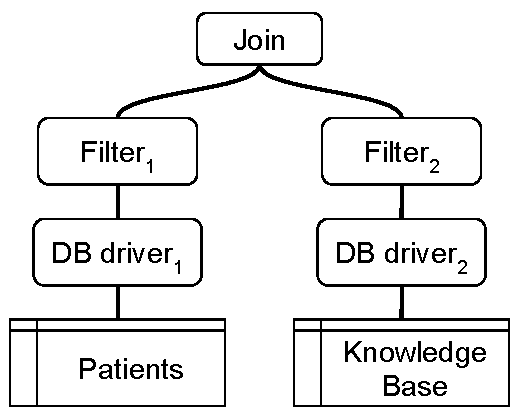
\includegraphics[width=0.4\textwidth]{./figures/design_pattern/qpu_graph_emergent_properties.pdf}
  \caption{QPU graph example}
  \label{fig:qpu_graph_emergent_properties}
\end{figure}

A \textit{QPU-based} query processing system is a directed acyclic graph (DAG).
Graph nodes are query processing unit instances.
Edges represent potential query request - response steam relations between QPUs.
A directed edge from $QPU_a$ to $QPU_b$ indicates that $QPU_a$ can send query requests to $QPU_b$.
When $QPU_a$ sends a $QPU_b$ a query request to $QPU_b$, a stream of query results with the opposite direction is established between them.

Leaf nodes (nodes with no outgoing connections) are always database driver QPUs.
Queries enter the QPU graph through root node (nodes with no incoming connections).
\todo{ref}

The capabilities of a QPU-based query processing system are emergent from the functionalities of the QPUs at its node, as well as the
graph topology.
For example, consider the QPU graph depicted in Figure~\ref{fig:qpu_graph_emergent_properties}:
\begin{itemize}

  \item $DB$ $driver_1$ can process queries with the form:
  {\obeylines\obeyspaces
  \texttt{SELECT SelectExpression from Patients TIMESTAMP TimestampExpression
  }}
  where $SelectExpression$ can contains one or more attributes of the $Patients$ table.

\item $DB$ $driver_2$ can process queries with the form:
{\obeylines\obeyspaces
\texttt{SELECT SelectExpression FROM KnowledgeBase TIMESTAMP TimestampExpression
}}
where $SelectExpression$ contains one or more attributes of the $KnowledgeBase$ table.

\item $Filter_1$ can send downstream queries to $DB$ $driver_1$
and apply a filter to its input stream.
Therefore, $Filter_1$ can process queries of the form:
{\obeylines\obeyspaces
\texttt{SELECT SelectExpression FROM Patients
        WHERE PredicateExpression
        TIMESTAMP TimestampExpression
        }}
where $SelectExpression$ and $PredicateExpression$ can use attributes of the $Patients$ table.

\item Similarly, $Filter_2$ supports queries of the form:
{\obeylines\obeyspaces
\texttt{SELECT SelectExpression FROM KnowledgeBase
        WHERE PredicateExpression
        TIMESTAMP TimestampExpression
        }}
where $SelectExpression$ and $PredicateExpression$ can use attributes of the $KnowledgeBase$ table.

\item $Join$ can send downstream queries to $Filter_1$ and $Filter_2$
and join the two input streams based on a given attribute.
Assuming that the $Patients$ and $KnowledgeBase$ tables have a common attribute, $symptoms$,
$Join$ can process queries of the form:
{\obeylines\obeyspaces
\texttt{SELECT SelectExpression
        FROM Patients JOIN KnowledgeBase ON Patients.symptoms = KnowledgeBase.symptoms
        WHERE PredicateExpression
        TIMESTAMP TimestampExpression
        }}
where $SelectExpression$ and $PredicateExpression$ uses attributes from both tables.

\end{itemize}

\todo{ref}

\subsubsection{QPU-graph topology rules}
topology cannot be arbitrary

rules that stem from the query processing units' functionalities

non-exhaustive list,
For each QPU class can be generalized to two types of rules:
(1) number of downstream connections, and (2) the \textit{query processing capabilities} of the downstream connection

\begin{itemize}
  \item All QPU graphs mush have database driver QPUs as their leaves.
  Database drivers generate the initial streams that any other QPU builds on.

  \item Most QPUs in the relational operator and derived state groups must have a single downstream connection.
  Exception consists relational operator QPUs that by definition operate on more that one input streams, such as join QPUs.

  \item A materialized view QPU must have a downstream connection that can provide a stream of updates on the query
  that defines the materialized view
  In more detail, the downstream connection of a materialized view QPU must be the root of a subgraph that
  \begin{itemize}
    \item Can process the query the is the materialized view's definition.
    \item Supports \textit{interval queries} on that query.
  \end{itemize}
  \todo{use existing example}

  \item Similarly, a secondary index QPU must have a downstream connection that can provide a stream of updates on the
  attribute that QPU is configured to index.

  \item A cache QPU must have at least on downstream connection.
  This connection can be towards any valid sub-graph.

  \item Similarly, a filter QPU can be connected to any valid sub-graph.

  \item A partition manager QPU must have one or more downstream connections to derived state QPUs that implement
  partitions of a derived state structure.
  In more detail:
  \begin{itemize}
    \item All downstream connection must be of the same QPU class

    \item They must be configured as partitions of a logical global derived structure, based on a single partitioning key.
  \end{itemize}

  \item A load balancer QPU must have one or more downstream connections, and the \textit{intersection} of the queries
  supported by these downstream QPUs must be non empty.
  Because any of the downstream QPUs can process the queries at the intersection of their supported queries, the load
  balancer QPU can perform distribute these queries among its downstream connections.
\end{itemize}

\subsection{Computation model}
\label{sec:computation_model}

% In this section we present how QPU-based query processing systems process queries.
% We first present an overview of the computation model \ref{sec:computation_model}, and then ...

The query processing unit computation model combines elements from microservice architectures and stream processing systems.
Similar to stream processing systems,
query processing units operate on input streams either to incrementally update their state, or to perform query processing
computations.
Similar to microservices architectures, any stream is initiates as a response to a \textit{service request}.

\medskip

The computation run by a QPU-based query processing system directly emerges from the QPU specification.
We describe this collective computation by describing the execution of a generic query $q$ by a QPU graph.
Given a query $q$, the query processing function of a QPU $Q$ at the root of a QPU graph sends query request to
downstream connection in order to initialize input stream required for processing the query.
The QPU performs a computation on the input streams, potentially also involving its state, and emits the results at its
output stream.
The same process is performed at each of the downstream connection of $Q$, and their downstream connection, propagating
downwards through the QPU graph.
This creates a \textit{query execution sub-graph} composed of the QPUs that participate in the processing of $q$.

The leaves of this sub-graph are QPU that can process their given queries without sending downward query requests.
This includes database driver QPUs, and derived state QPUs.
These QPUs become the leaves of $q$'s execution sub-graph.
Leaf QPUs produce output streams that are then received as input stream at \textit{upstream QPUs}.
Progressively, each non-leaf QPU in the query execution sub-graph receives an input stream for each query request sent,
and produces itself an output stream.
Finally, $Q$ calculates the response for $q$ and emits it as its output stream.
We call this type of QPU graph computation \textit{query execution mode}.

\medskip
our ````````````````````````''''''''''''''''''''''''
The same process is performed for incrementally updating secondary index and materialized view QPUs (\textit{state maintenance mode}).
There are the following differences between query execution mode and state maintenance mode:
\begin{itemize}
  \item Query execution happens in response to a client query,
  while state maintenance happens in response to the initialization of a secondary index of materialized view QPU.
  \item The goal of query execution is to process a client query,
  while the goal state maintenance is to establish a long running stream of notification for corpus updates.
  \item The root of a query execution sub-graph is one the QPU graph root nodes,
  while the root of a state maintenance sub-graph is a derived state QPU.
\end{itemize}

\medskip

Based on the above description, the computation run of a QPU-based processing system can be characterized as a
\textit{bi-directional dataflow computation}.
For a given query or state maintenance execution,
query requests flow downwards through the QPU graph, defining an execution sub-graph.
Response streams flow upwards through that sub-graph, each stream corresponding to an edge defined by a query request.

\medskip

Finally, query processing units are multi-threaded:
a QPU can process multiple queries in parallel.
Therefore, multiple different query execution and state maintenance sub-graph can co-exist in parallel in the same QPU
graph.

\subsection{Query execution}

\subsubsection{Query parse tree}

The first of a QPU's query processing function is to parse the query request to a form that can be used for query processing.
This form is a \textit{parse tree}.

A parse tree is constructed by applying the QPU query language's grammar to a given query string.
More specifically, a parse tree is composed to three types of nodes:
\begin{itemize}
  \item \textbf{Atoms}, which include keywords of the query language ($SELECT$, $FROM$ etc.),
  identifiers, such as table or attribute names, constants, operators and tokens.
  Atoms are leaf nodes of the parse tree.

  \item \textbf{Syntactic categories}, which are constructs built from other syntactic categories, or atoms,
  follow the query language's grammar rules ($SelectExpression$, $TableExpression$ etc.)
  Syntactic categories are internal nodes of the parse tree
\end{itemize}

Given a query string $s$, a parse tree is constructed by parsing $s$ using the query language grammar rules.
\todo{ref parsing algorithms}

\subsubsection{Query processing capabilities tree}

In this section we present the \textit{query processing capabilities tree} (QPC tree)
The QPC tree represents the \textbf{set of all query parse trees that a QPU can process}.

To achieve that, we introduce an additional typo of tree node, the \textbf{conjunction} \todo{better name??}.
Conjunction nodes essentially express the different branches of a syntax rule.
For example, the rule:
{\obeylines\obeyspaces
\texttt{
PredicateExpression  ::=  PredicateExpression OR PredicateExpression |
~~~~~~~~~~~~~~~~~~~~~~~~~~PredicateExpression AND PredicateExpression |
~~~~~~~~~~~~~~~~~~~~~~~~~~NOT PredicateExpression |
~~~~~~~~~~~~~~~~~~~~~~~~~~Term Op Term
}}

can be represented as \todo{do the tree}.


.. Present the trees in the orders example ..

Each QPU has a QPU tree, which is parts of its configuration state.
Stores the QPC trees of its neighbors as part of its local view state.

It is used for two purposes
\begin{itemize}
  \item The QPU uses determines if it can process a given query by the parse tree of the given query ``fits'' its QPC tree.
  \item The QPU generates downstream query requests using the QPC trees of its downstream connections, by performing a
  trimming operation.
\end{itemize}




% Given $q$, the query processing function of a QPU $Q$ at the root of the QPU graph sends query request to some its
% downstream connection, in order to initialize input stream required for processing the query.
% Upon receiving a query request from $Q$, each of its downstream connection performs the same process.
% In that way, query requests are propagated downwards through the QPU graph, creating a \textit{query execution sub-graph}
% composed of the QPUs that participate in the processing of $q$.

% As query requests requests are propagated downwards, expanding the $q$'s execution sub-graph, eventually some QPUs can
% process their queries without sending further query requests downwards.
% This occurs in database driver and derived state QPUs.
% The leaves of this sub-graph are QPU that can process 
% This includes database driver QPUs, and derived state QPUs.
% These QPUs produce output streams that are then processed as input stream at \textit{upstream QPUs}.

% Progressively, each non-leaf QPU in the query sub-graph receives an input stream for each query request sent,
% and produces it self an output 


% We describe how a QPU graph processes a given query using the example of Figure~\ref{fig:qpu_graph_emergent_properties}.

% Consider the query:
% {\obeylines\obeyspaces
% \texttt{Q = SELECT CustomerName, CustomerEmail, OrderID
%         ~~~~FROM Customers
%         ~~~~INNER JOIN Orders ON Customers.OrderID = Orders.OrderID
%         ~~~~WHERE Orders.OrderDate >= 2020-08-20 AND Orders.OrderDate < 2020-09-02
%         ~~~~TIMESTAMP FROM LATEST TO LATEST
%         }}





% - queries / control messages flow downwards.
% - responses flow upwards through the sub-graph defined by the queries
% - (each query establishes a sub-graph - actually a tree - to be used by that particular query);
% - Updates (independently) also flow upwards

% As described in the previous sections, query processing units can collaborate by invoking the query API of one another.
% QPUs can be composed in DAG hierarchies in which parent units can invoke the query API of their child units.
% Query responses for both snapshot and persistent queries are streams of results.
% Communication between QPUs thus uses a combination of the remote procedural call model (query API invocations) and the stream-processing model (query responses).

% Clients perform queries by invoking the query API of units at root nodes of the graph.
% Once a QPU receives a query, it determines whether it can directly process it, for example by performing lookups at its indexing structures,
% and if that is the case it responds with the query result.
% In case the query processing computation requires partial query results from its child units, the unit invokes the query API of those units with the appropriate sub-queries.
% Sub-query results are received and processed through the unit's callback function.

% This process is recursively performed at each query processing unit.

% Therefore, the computation that runs in QPU a graph can be modeled as a bidirectional data-flow computation.
% Queries flow downwards through the graph, are incrementally split into sub-queries, and processed across the graph.
% Sub-query results flow back upwards, are incrementally processed, and eventually produce the results to the initial query.

% The same computation model is used for index maintenance.
% We have extended the query interface semantics so that the query API can be used to subscribe to notifications for corpus updates, and query results can encode these updates.
% Using this mechanism, units with indexing functionalities can subscribe to corpus updates by invoking the query API of QPUs that provide this functionality.
% We describe this mechanism in more detail in Section \ref{subsec:query_classes}.


% The QPU graph runs a distributed bidirectional data-flow computation.

% A client performs a query $Q_c$ by invoking the query API of a query processing unit at the root of the graph.
% As described in Section~\ref{subsec:qpu}, the QPUs query processing computation can read from the unit's state,
% or perform downstream queries to QPUs at its child nodes.

% When a downstream query is performed, this process is recursively executed at each unit whose query API is invoked.
% Though this mechanism, $Q_c$ is incrementally transformed to sub-queries which flow downwards through the QPU graph,
% invoking computations at different nodes.
% Sub-query results are returned through the QPU streams established from query API invocations, and flow upwards
% through the graph.
% These results are incrementally processed, potentially updating the state of different QPUs, and eventually
% produce the initial query results, which are returned to the client.









% \section{QPU Composition: Constructing QPU-based query engines}
% Here, describe how query engines are constructed using instances of QPU classes.

% A query engine is a directed acyclic graph (why?) with QPUs as nodes.

% Describe the QPU-specific topology properties that the graph must satisfy in
% order to be functional:
% \begin{itemize}
%   \item All leaves must be QPUs of the datastore driver class.
%   Also, datastore driver QPUs cannot be nodes other than leaves.
%   \item TODO
% \end{itemize}

% \section{Computation Model}
% Describe the bidirectional data-flow computation.
% \begin{itemize}
%   \item Control messages (queries) flow downwards.
%   \item Responses flow upwards through the sub-graph defined by the control
%   (each query establishes a sub-graph - actually a tree - to be used by that
%   particular query);
%   \item Updates (independently) also flow upwards.
% \end{itemize}


% % \section{The consistency guarantees of QPU-based query engines}
% % TODO: What mechanism are needed so that QPUs can guarantee internal consistency?
% % What about session consistency guarantees?

% \section{Discussion}

% % -- point to make -- unified subscription and snapshot

% % It is known that query execution can be represented as a tree.
% % Base data are at the tree's leaves, tree nodes are relational operator such
% % as filter, joins and aggregations, and query result are at the root of the tree.
% % Each operator receives an input stream of records, performs a transformation on the, and emits a output stream of record.
% % This results to a data-flow computation in which data items flow upwards through the tree and are progressively transformed
% % to the query execution results.

% % Computation tasks vs architecture components

% % Our approach is based on three simple insights:
% % \begin{itemize}
% %     \item \textbf{Index-based distributed query processing is composed of basic, primitive tasks.}
% %     The most simple query engine design is a component that scans the corpus dataset and selects the data items which match a given query.
% %     When queries for certain attributes are frequent or require low response time, secondary indexes can be materialized for those attributes.
% %     Even when indexes are partitioned and distributed across the system for scalability, the basic components of an indexing system remains the same: index data structures that collaborate through appropriate index maintenance and query processing protocols to implement distributed indexes.
% %     Additional query processing functionalities such as multi-attribute queries, joins or federated queries across multiple corpus can be implemented using operators that build on top of these components.
% %     Finally, caching can be used to further improve response time for certain queries.

% %     \item \textbf{Primitive query processing tasks can be encapsulated by a common query processing component abstraction.}
% %     Each of the described tasks can be encapsulated by a query processing component abstraction with two properties: an API for responding to queries, and a callback function.
% %     For example, index data structures in general implement three basic functions: LOOKUP, INSERT, DELETE.
% %     The query API can encapsulate the LOOKUP function, while the callback function can express the task of index maintenance, receiving corpus updates and updating the index accordingly, and therefore encapsulate INSERT and DELETE.
% %     As another example, a cache on top of an index structure should be able to respond to the same queries as the underlying index, and therefore can be encapsulated by a query processing component with the same query API.
% %     Similarly, its callback function can express the task of receiving query results in case of a cache miss, and updating the cache.
% %     This concept can be generalized to represent other query processing components including bloom filters, materialized views, and streaming operators.

% %     \item \textbf{Query processing components need to cooperate to implement complex query processing tasks.}
% %     As an example, a caching component requires the ability to forward queries to other components, such as indexes, when cache misses occur.
% %     Similarly, a distributed indexing system, in which indexes are partitioned and distributed across system nodes, can be implemented using indexing components with the help of an additional component responsible for implementing a partitioned LOOKUP operation, by collecting and aggregating partial LOOKUP results.
% % \end{itemize}

% % Based on these observations, we introduce a query processing component abstraction, called the \textit{Query Processing Unit} (QPU).
% % We have designed a generic query API and callback function interface with the aim of encapsulating multiple different query processing components.
% % Query processing units may have internal state for facilitating query processing, or be stateless.
% % Additionally, QPUs have the ability to invoke the query API of one another, and thus interoperate for query processing.


\chapter{Proteus: Towards application specific query processing systems}
\label{ch:proteus}
The goal of this chapter is to present Proteus, a framework for facilitating
the construction and deployment of QPU-based query processing systems.

This includes:
\begin{itemize}
  \item Presenting the library of QPU implementations offered by Proteus.
  \item Describing the additional mechanism offered by Proteus for deploying and
  connecting.
  \item Reporting on subjects including rules of QPU composition (incompatible
  topologies), (steps towards automatic cost-model based deployment plans for
  QPU graphs)*, and implementation details.
\end{itemize}

Having presented the QPU characteristics, the principle of composing QPUs in a DAG, and the graph's computation model,
the goal of this chapter is to concretely.

\section{QPU query processing capabilities}

Each QPU is responsible/capable of processing queries in a specific space. These capabilities depend on:
\begin{itemize}
  \item The QPU's functionality (class).
  \item It's configuration.
  \item It's child connections in the graph.
\end{itemize}

QPUs maintain metadata (state) that describe their own capabilities, as well as their knowledge of the capabilities of
their child connections.

In this section we describe the format of the query processing capabilities state. We defer the description of how QPUs
populate this state for the following section.

\section{Distributed query processing protocol}
In this section we present the protocol that QPUs use to retrieve intermediate query responses for a given query by
sending sub-queries to child QPUs.

In detail, we present the algorithms for:
\begin{itemize}
  \item Determining if the QPU can process a given query locally, or if the QPU needs to forward parts of the query
  processing computation to the QPU graph.
  This can be done by sending sub-queries to its child connections.
  \item How a QPU uses its knowledge of the query processing capabilities of its child connections to generate and send
  sub-queries.
\end{itemize}

This protocol runs locally at each QPU and requires no central coordination.

\section{Configuration Dissemination}
In this section we describe how QPUs build/populate the query processing capabilities state.

Overview:
\begin{itemize}
  \item In the case of the index QPU, its configuration explicitly describes which queries can be processed locally
  (using the index).
  \item For other QPUs (e.g. filter, cache), their capabilities depend on the capabilities of their child connections.
  For example, if a cache QPU is connected to an index QPU, it inherits the query capabilities of that QPU.
\end{itemize}

Here, we also define the operation of combining the capabilities of more than one QPUs (a QPU uses that operation to
calculate its capabilities given its configuration and the capabilities of its children)

% \subsection{Configuration propagation API}
% Νο 5.3.2

\section{QPU Library}
Describe the implementation-specific details, assumptions, and limitations of
the QPU classes provided by Proteus.

\subsection{Datastore driver}
\subsubsection{Backend data stores}

\subsection{Filter}

\subsection{Index}

\subsection{Cache}

\subsection{Multiplex \ De-Multiplex}

\subsection{Conjunction / Disjunction}


\section{Constructing QPU-based query engines}
Demonstrate the use of the QPU classes described above for constructing query
engines.

\subsection{QPU graph topology rules}
Summarize the rules that apply to the construction of QPU graphs.
This includes:
\begin{itemize}
  \item Components (caches, filters) that do not have multiplexing logic and can
  only be put on top of one QPU.
  \item How the QPU graph is connected with the data storage tier via data store
  driver QPUs.
\end{itemize}

In this chapter, include rules that are not inherent to the QPU design, but
rather are due to the implementation choices.

Rules that are inherent to all QPU graphs, should be stated in
% Chapter~\ref{ch:design_pattern}.


\subsection{Reference QPU architecture patterns}
Demonstrate in detail how Proteus can be used to build a number of query engine
architectures.

Reference architectures can be categorized by two characteristics: (1) the query
processing components they use (filter-only, filter-and-cache, index-base, ..),
and (2) the storage tier architecture they target (single database instance,
sharded database, replication, federation)

For (2) we will take a ``zooming out'' approach: each reference architecture
building on top of the previous one.

\subsubsection{Partitioned index}

\section{Fault tolerance}
Describe the mechanisms provided by Proteus for tolerating faults during query
processing.
\begin{itemize}
  \item Lost or re-ordered stream records.
  \item Mid-query QPU crash.
  \item Partitions.
\end{itemize}

\section{Implementation}
Report on the implementation of different components of Proteus, including:
\begin{itemize}
  \item The framework used for communication between QPUs.
  \item How streams are implemented.
  \item ...
\end{itemize}


% TODO: title
\chapter{Evaluation}
\label{ch:evaluation}
In this chapter, we aim to validate our analysis of the trade-offs involved in query processing state placement decisions,
and to evaluate the effectiveness of our design and prototype implementation in providing an effective mechanism to applications
for navigating these trade-offs.

This evaluation consists of two parts.
The first part (\S\ref{sec:eval_1}) is based on the case study of a read-heavy web application, presented in Section~\ref{sec:lobsters}.
It focused on the placement of a materialized view,
and examines two placement options: in the data center, close to the corpus, or at the edge close to the clients.
The aim of the first part is to answer the following questions:

\begin{itemize}

  \item What is the overhead of materializing state in Proteus, directly over the data storage tier?
  (Section~\ref{sec:eval_query_processing_perf})

  \item What improvements in query processing performance can be achieved by placing materialized state close to clients?
  (Section~\ref{sec:eval_query_processing_perf})

  \item What are the penalties in freshness incurred when placing materialized state away from the data storage tier
  (Section~\ref{sec:eval_freshness})?
  How is freshness affected by load (\S\ref{sec:eval_freshness_throughput}) and round-trip time between
  sites (\S\ref{sec:eval_freshness_rtt})?

  \item What additional data transfer costs result from materialized state placed close to clients receiving updates?
  (Section~\ref{sec:eval_data_transfer})

\end{itemize}

The second part (\S\ref{sec:eval_2}) of the evaluation is based on the case study of federated query processing on a multi-cloud
corpus, presented in Section~\ref{sec:zenko}.
In this part we examine three partitioning and placement configurations for a multi-cloud secondary index.
We compare the three configurations under different types of workloads, and evaluate three metrics:
query processing performance, freshness and data transfer costs.

The aim of the second part is to (1) demonstrate the expressiveness of the QPU approach,
by deploying and comparing three query engine configurations across 3 data centers without any changes to the client application and the storage tier,
and (2) validate that by controlling the configuration of QPU-based query engines,
applications can navigate the trade-offs of geo-distributed query processing and optimize for different criteria according to their needs.


\section{Placing materialized views at the edge}
\label{sec:eval_1}

\subsection{Experimental scenario}
\label{sec:eval_scenario}

The evaluation in this section is based on the case study presented in Section~\ref{sec:lobsters},
which describes the Lobsters \cite{lobste:rs} web application.
We choose this application for the following reasons:
\begin{itemize}
\item It is characterized by a query-heavy workload that requires the materialization of derived state,
and derived state is updated by a stream of small updates.
This make Lobsters suitable for evaluating the efficacy of our design and prototype implementation in
navigating the trade-offs of query processing state placement,
by examining the effect of different placement schemes in query performance and query result freshness.

\item It open-source \cite{lobsters:source},
allowing us to examine the application's interaction with the database in which it stores its state,
and statistics about the application's data usage patterns are available \cite{lobste:stats}.

\item It resembles a class of popular large-scale web applications, such as Reddit and Hacker News.
\end{itemize}

\bigskip
\noindent
In Lobsters, users post, comment, and vote on ``stories''.
Each story is associated with a ``hotness'' value that indicates how popular it is.
Stories are ranked by hotness;
the stories with the highest hotness value appear on the front page.
The hotness value of a story depends on parameters such as the number of votes for the story,
the number of comments, and the hotness of those comments.
Various operations, such as voting or commenting on a story, modify the hotness value.
Computing the hotness value when it is queried would impose a prohibitive delay on queries
% It is prohibitively expensive \cite{gjengset:noria} to compute the hotness value of stories during queries.
In particular, serving the Lobsters' front page requires computing the hotness of every story in order to rank them.
That is why the Lobsters application adds an additional column to the $stories$ table which stores a pre-computed
hotness value for each story.
The application updates the value of the hotness column when operations are performed,
such as upvoting or downvoting a story, or adding a comment to a story.

For this evaluation, we consider a version of the Lobsters application, that consists of two operations:
voting for stories, and requesting the front page.
We choose this simplified model of the application because it gives us better control over the properties of the workload
for the purposes of this evaluation,
while also capturing the aspects of the Lobsters application that make is suitable for this evaluation.

In particular, we consider the following database schema:

\begin{lstlisting}[caption={Simplified Lobsters schema used in this evaluation.}]
TABLE users (id bigint, username varchar(50))
TABLE stories (id bigint, user_id bigint, title varchar(150), description mediumtext, short_id varchar(6));
TABLE votes (id bigint, user_id bigint, story_id bigint, vote tinyint);
\end{lstlisting}

The front page is a listing of the 25 most highly ranked stories, including their title, author, and vote count.
In the statistics provided by the Lobsters administrators, the front page operation constitutes 30.1\% of client requests,
and voting on stories constitutes 0.5\% of client requests.
The workload used for this evaluation consists of 95\% front page operations, and 5\% voting operations, unless otherwise specified.

\begin{table}[H]
\centering
\begin{tabular}{|c||c|c|c|c|c|c|}
\hline
Number of votes & [0-10) & [10-20) & [20-30) & [30-40) & [40-50) & [50-60) \\
\hline
\% of stories & 41.1 & 40.3 & 11.3 & 4.2 & 1.6 & 1.3 \\
\hline
\end{tabular}
\caption{Distribution of votes to stories in the Lobsters statistics \cite{lobste:stats}.}
\label{tab:votes_per_story}
\end{table}

According to the available data \cite{lobste:stats}, most stories (81.4\%) receive between 0 and 20 votes,
while about 7\% receive 30 votes or more.
Our experiments show that when votes follow this distribution,
very few votes are performed on the stories on the front page to have meaningful impact on query result freshness.
To address that, we use a more skewed distribution:
We configure 60\% of votes to target the 25 stories in the front page, and 40\% to follow the distribution shown in Table~\ref{tab:votes_per_story}.

\begin{figure}[H]
  \centering
    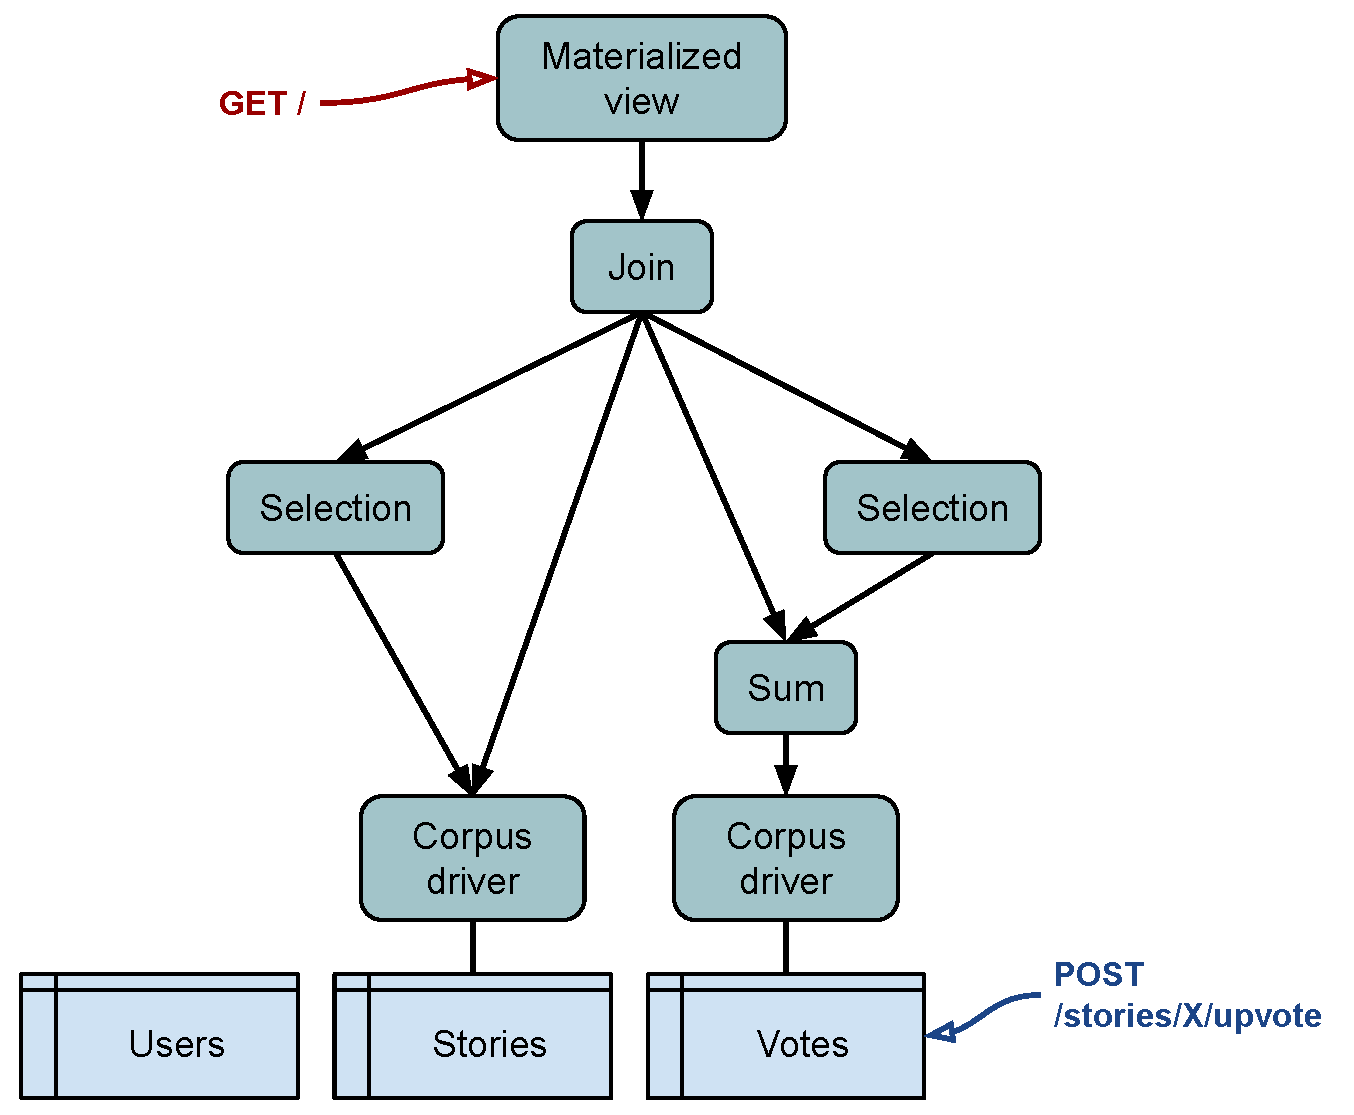
\includegraphics[scale=0.5]{./figures/evaluation/lobsters_architecture_eval.pdf}
  \caption{QPU graph used for this evaluation. The Materialized view QPU computes the vote count for each story,
  and joins it with the corresponding record from the $stories$ stable.
  The ``GET /'' request indicates the front page operation, and the ``POST /stories/X/upvote'' request indicates the operation of voting up story X.}
  \label{fig:eval_lobsters_qpu_arch}
\end{figure}

\bigskip
\noindent
The evaluation uses the QPU graph depicted in Figure~\ref{fig:eval_lobsters_qpu_arch} to maintain a materialized view that
pre-computes the vote count of each count and joins it to the corresponding record of the $stories$ table.
The materialized view is defined by the following query:

\begin{lstlisting}[caption={Definition of the materialized view maintained by the QPU graph shown in Figure~\ref{fig:eval_lobsters_qpu_arch}.}]
SELECT id, author_id, title, url, vote_count
FROM stories
JOIN (
  SELECT story_id, SUM(vote) as vote_count
  FROM votes
  GROUP BY story_id
) view
ON stories.id = view.story_id
\end{lstlisting}

This simplifies both the vote and front page operations compared to the baseline Lobsters implementation:
the vote operation does not need to explicitly update the vote count of the given story, as this
is performed by the QPU graph,
and the front page operation can be served from the materialized view.

In the actual QPU graph deployed for the experiments, each Selection QPU is merged with its downstream connection,
in a single unit that performs both functionalities.
In addition, the Materialized View is merged with the Join QPU.

The Materialized view QPU implementation used in these experiments stores its state in a MariaDB instance.
This is a separate instance from the one that is used the Lobsters database.
It is deployed alongside and only accessible by the Materialized view QPU.
The choice of using the same database both as the baseline and for storing the materialized view is aimed at eliminating
the effect of the database performance from the evaluation results,
providing a comparison that isolates the effects of placement.

Finally, we create an index on the table that implements the materialized view in order to support efficient retrieval of
the stories with the highest vote count.

\bigskip
\noindent
We consider a system topology consisting of two geographically distant sites:
The Lobsters application is deployed on one site, called server site,
and clients are located on another site, called client site.
Round-trip time between these two sites is 80 ms.
This corresponds to a scenario in which the Lobsters web application is deployed in a data centers in North America,
and clients are located in Europe \cite{pbailis:hats}, or vice versa.

Our experiments  make use of the ability to place QPUs strategically in the system topology.
We use two placement schemes:
One in which the Materialized view QPU is placed at the server site, and one in which it is placed at
the client site.
We evaluate the effects and trade-offs of materialized view placement by comparing these two placement schemes.


\subsection{Experimental Setup}
\label{sec:eval_setup}

While the actual Lobsters Ruby-on-Rails application is open-source,
we use a simplified version of it in order to isolate its interaction with the database.
We implement an adapter that translates front page and vote requests to the queries that the real
Lobsters application would issue, and issues those queries either to the Lobsters database (MariaDB),
or MariaDB and Proteus, depending on the experiment configuration.
This allows us to isolate the interaction between the application and the database, which is the focus of this work,
and remove other tasks that the Lobsters application performs, which quickly become a bottleneck.

We implement this adapter as a server-side component:
it is deployed along with the database on the server site, and plays the role of a simplified web server:
It exposes a gRPC endpoint, similar to the QPU gRPC server, and clients issue operations to it as RPC requests.
We choose this configuration because our initial experiments showed that issuing a large number of concurrent transactions
to MariaDB under a 80 ms client-server round-trip time results in errors both in the database,
and the Go MySQL library.

\bigskip
\noindent
\textbf{Workload generation.}
We implement a workload generator \cite{lobsters:bench} that is responsible for issuing
requests to the Lobsters adapter.
The workload generator uses an open-loop model \cite{schroeder:cautionarytale}:
it creates requests based on a target load (requests submitted per second) value;
each request is executed by a separate thread (creating and destroying threads are low-cost operations because threads are
implemented as Goroutines).

In addition, the workload generator measures throughput and response time.
We define response time as the delay that a client application experiences between issuing a request and receiving the
corresponding response.
To capture the variance of response time, we use a histogram data structure provided by the Go implementation of gRPC \cite{grpcgo:histogram}
that accumulates values in a histogram with exponentially increasing bucket sizes, in order to compute response time percentiles.

Our experiments show that while the open-loop design is effective at generating the target load
both under low and high client-server round-trip times (in closed-loop designs, high round-trip times result in lower offered load),
it results in a positive feedback loop effect above a certain load threshold:
When the system starts not being able to handle the offered load, response time increases.
However, the workload generator keeps generating requests, and, because of the increased response time,
more requests are ongoing concurrently.
This puts more load in the gRPC server, increasing the response time even more.
Even a small initial increase in response time triggers this feedback loop,
which eventually increases response time more and more during the duration of the benchmark.
To address this problem, we extended the workload generator with a mechanism that limits the overall number of requests
(and thus threads) that can be ongoing at a given point in time, to a configuration-specified bound.
When the bound is reached, additional requests need to wait for ongoing requests to be completed.

The concurrency bound mechanism is effective in avoiding the positive feedback loop effect.
However, it also means that when running a benchmark for a given target load we need to specify a bound in the number of
concurrent threads that is sufficient for reaching the target load.
If the bound is too low, then the workload generator cannot generate enough load, but and but response time does not
increase because the delay caused by waiting for available threads is outside of the response time measurement.

\bigskip
\noindent
\textbf{Freshness.} The materialized state maintained by the Materialized view QPU updated asynchronously.
As a result, queries served from the materialized view might reflect state that is stale relative to the database state.
The staleness of the materialized state is impacted by its placement:
Placing the Materialized view QPU at the client side entails a minimum 40 ms communication latency to the materialized view
(80 ms round-trip time between sites).
Throughout the rest of this chapter, we consider the terms freshness and staleness equivalent and use them interchangeably.

One of the aims of this evaluation is to quantify how stale query results become.
To achieve that, we measure the staleness of the results returned by the front page operation,
using the following metrics:
\begin{itemize}
  \item \textbf{Update latency:} The delay between a vote being committed in the database, and the materialized view being
  updated with the new vote count.
  \item \textbf{Returned version:} The difference, in number of versions, between the version of a story record returned by a query,
  and the version that would have been read by querying the Lobsters database instead of the materialized view.
\end{itemize}

We collect these metrics as follows.
For each vote operation, the Lobsters database logs the timestamp at which the corresponding transaction commits;
the database then includes the commit timestamp the update record that it publishes to the QPU graph.
When the update record reaches the Materialized view QPU, the QPU stores the commit timestamp in an
``update log'' table.
Moreover, the Materialized view QPU logs the timestamp of each view update in the update log,
and the timestamp at the start of each query, in a ``query log''.

At the end of a benchmark run, the Materialized view QPU performs a post mortem analysis:
The update latency for each vote is computed by subtracting the update timestamp from the commit timestamp.
The returned version for each front page story is computed by comparing the update and query logs.

A limitation of this mechanism is that it requires comparing timestamps taken on different servers.
To address that, in the benchmarks in which we take freshness measurements,
we deploy all system components (Lobsters database, QPU graph, workload generator) as containers,
on a singly physical machine.
Because they share a single OS kernel, all timestamps used for computing freshness metrics are based
on the host operating system's clock, and thus can be meaningfully compared.
We use the Linux tc utility \cite{tc} to simulate the 80 ms round-trip time between sites,
despite all containers being deployed on a single server.

\bigskip
\noindent
\textbf{Hardware.}
Experiments were run on a cluster provided by the Laboratoire d'Informatique de Paris 6 (LIP6).
Each server consists of 2 Intel Xeon E5645 CPUs, each with 6 cores, 64 GB RAM, an 128 GB SSD disk, and a 4 TB HDD disk.

\bigskip
\noindent
\textbf{Configuration.}
The average ping latency between machines in the cluster is less than 1ms.
We simulate the two geographically distant sites by using the Linux tc utility \cite{tc} to add delay to outgoing packets.

For response time measurements, the Lobsters MariaDB instance and the QPUs, except the Materialized view QPU are deployed
on a single server on the server site, and the workload generator is on a server in the client site.
The Materialized view QPU is deployed on a separate dedicated server, either on the application or the client site,
according on the placement scheme being tested.
As described above, for the freshness measurements, all components are deployed on a single server.

Experiments run for 5 minutes unless otherwise specified, and we start taking measurements after an initial
``warmup period'' of 30 seconds.
Repeated runs have shown that results are stable and consistent across runs.


\subsection{Query processing performance}
\label{sec:eval_query_processing_perf}

\begin{figure}[H]
        \centering
        \begin{subfigure}[b]{0.24\textwidth}
            \centering
            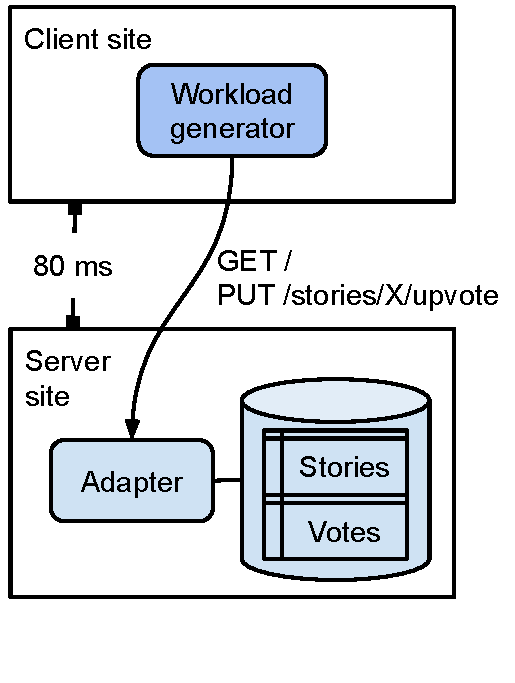
\includegraphics[width=\textwidth]{./figures/evaluation/evaluation_deployments_baseline_remote.pdf}
            \caption{Baseline/remote}
            \label{fig:deployments_baseline_remote}
        \end{subfigure}
        \hfill
        \begin{subfigure}[b]{0.24\textwidth}
            \centering
            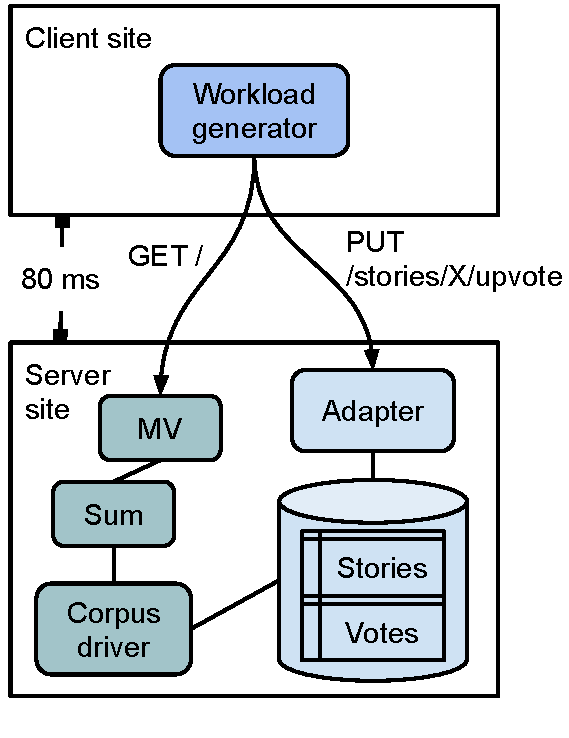
\includegraphics[width=\textwidth]{./figures/evaluation/evaluation_deployments_proteus_remote.pdf}
            \caption{Proteus/remote}
            \label{fig:deployments_proteus_remote}
        \end{subfigure}
        \hfill
        \begin{subfigure}[b]{0.24\textwidth}
            \centering
            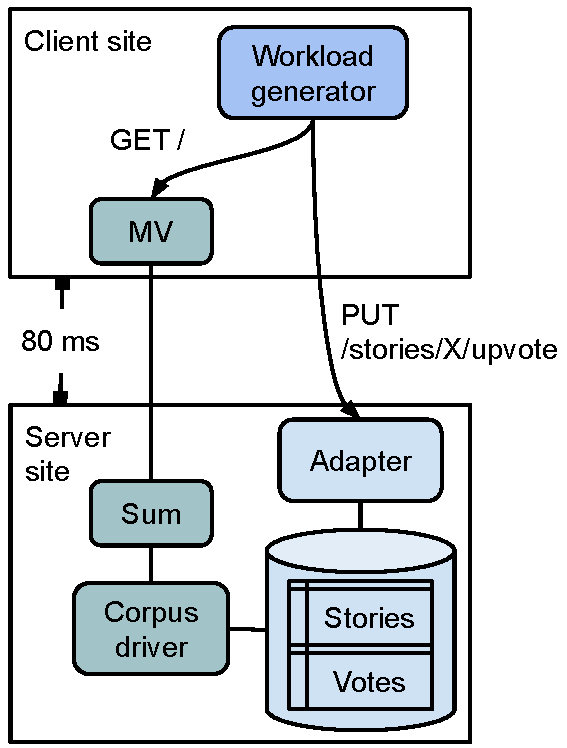
\includegraphics[width=\textwidth]{./figures/evaluation/evaluation_deployments_proteus_local.pdf}
            \caption{Proteus/local}
            \label{fig:deployments_proteus_local}
        \end{subfigure}
        \hfill
        \begin{subfigure}[b]{0.24\textwidth}
            \centering
            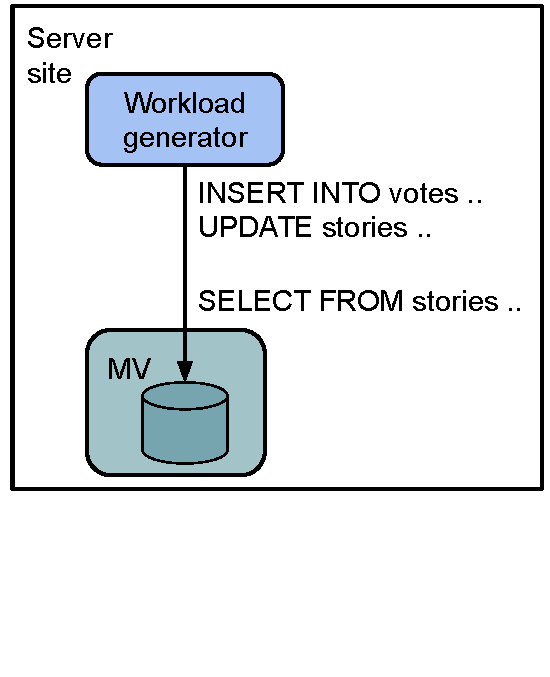
\includegraphics[width=\textwidth]{./figures/evaluation/evaluation_deployments_internal.pdf}
            \caption{Materialized-view-internal}
            \label{fig:deployments_mv_internal}
        \end{subfigure}
        \caption{Deployments used in this evaluation.}
        \label{fig:eval_deployments}
    \end{figure}

We compare three deployments that differ in how they store and calculate the per-story vote count,
and how they distribute computations and state across the nodes of the system (Figure~\ref{fig:eval_deployments})
\textbf{Baseline/remote} (Fig.~\ref{fig:deployments_baseline_remote}) is equivalent to the real Lobsters application:
it pre-computes and stores vote counts in a column of the Lobsters $stories$ table.
This serves as the baseline approach.
\textbf{Proteus/remote} (Fig.~\ref{fig:deployments_proteus_remote}) consists of the QPU graph shown in Figure~\ref{fig:eval_lobsters_qpu_arch},
deployed on the server site.
In \textbf{Proteus/local} (Fig.~\ref{fig:deployments_proteus_local}),the Materialized view QPU is deployed on the client site.
This is intended to evaluate the effect of placing the materialized view close the client.
We also compare with a deployment (\textbf{Materialized-view-internal}, Fig~\ref{fig:deployments_mv_internal}) in which the workload generator
directly issues request to the Materialized view QPU's state, bypassing the QPU's gRPC server
(the workload generator and materialized view are co-located on the same server).
This aims at providing an indication of the best performance the Materialized view QPU can achieve,
without taking into account its gRPC server (which we have identified as a performance bottleneck).

\begin{figure}[H]
\centering
  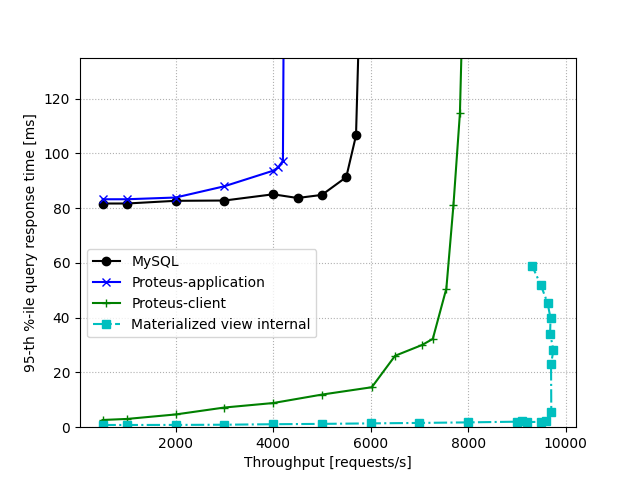
\includegraphics[width=0.7\textwidth]{./figures/evaluation/responseTime.png}
  \caption{Throughput vs 95th percentile query response time.}
  \label{fig:responseTime}
\end{figure}

Figure~\ref{fig:responseTime} shows throughput--query response time plots of these deployments.
The ideal throughput--response time curve would be a horizontal line with low response time.
The lower bound response time for Baseline/remote and Proteus/remote is 80 ms as this is the round-trip time between sites.
In reality, all systems' plots have a ``hockey stick'' shape:
latency remains relatively low until a point in which the system fails to keep up with the offered load.
After that point, the system cannot achieve additional throughput, and response time increases.

Materialized-view-internal scales up to 9800 requests/second,
outperforming both Proteus deployments.
This deployment is intended to evaluate the performance of the core functionality of the Materialized view QPU,
by directly translating front page and vote operations to accesses to the QPU's state using a thread pool,
bypassing the client-server gRPC communication.
Because of that, we conclude that the gRPC communication incurs a significant overhead in the throughout that
can be achieved by the system.

Proteus/remote scales to 4200 requests/second, which is a 24\% overhead compared to the baseline deployment (Baseline/remote),
which scales to 5500 requests/second.
Both those deployments eventually read and write state to a MariaDB instance.
The difference is how they translate requests to database accesses.
The adapter used in the Baseline/remote deployment uses a simple logic that translates vote and front page request to database transactions.
Conversely, the Materialized view QPU used in the Proteus/remote deployment contains more complex logic,
such as parsing received queries in SQL form, and receiving records from its input stream and updating the materialized view.
We attribute the observed 24\% overhead to the more complex logic.

In the Proteus/local deployment, query response time is significantly lower.
This is achieved because moving the Materialized view QPU to the client site removes the need for a costly round-trip to
the server site, and thus removes the 80 ms lower bound.
In addition, Proteus/local achieves a 28\% increase in achieved throughput compared to the Baseline/remote deployment
(we consider the maximum achieved throughput for which response time does not exceed 20ms and 100ms respectively).
We attribute this improvement to the lower concurrency required to generate the same load in Proteus/local
compared to Proteus/remote and Baseline/remote.
In more detail, offering a certain load (volume of requests/second) requires creating a number of concurrent client threads,
each performing a request.
When the round-trip time between sites is 80 ms, each of these threads executes significantly longer compared to
when the round-trip is just a few milliseconds.
As a result, offering a given amount of load in the Proteus/remote setup results in a significantly greater number
of threads, and thus open connections to the QPU's gRPC server, than in the Proteus/local setup.
If the number of connections that can be opened is not bounded by a connection pool, this overloads the QPU's gRPC server,
significantly increasing response times.
When a connection pool is used, each requests needs to wait for an available connection,
again increasing the end-to-end response time experienced by the client.

\medskip
\noindent
\textbf{Conclusion.} Our experiments confirm that placing materialized views closer to the client benefits read-heavy applications
by removing costly round-trip communication across sites, and achieves scalability improvements.
This results is expected, and shows the benefits that can be achieved by enabling this placement.


\subsection{Freshness}
\label{sec:eval_freshness}

\subsubsection{Freshness vs Throughput}
\label{sec:eval_freshness_throughput}

In the actual Lobsters application (and the Baseline/remote deployment),
the vote count is maintained in the $stories$ table.
Because of the consistency guarantees of MariaDB,
the vote count of a story, is always up-to-date with the state of the $votes$ table.
However, maintaining a materialized view placed at a remote site synchronously adds prohibitive overhead to write operations.
Because of that the QPU graph in this evaluation maintains the materialized view asynchronously, and, as a result,
its state might be stale relative to the state of the corpus.

In this section, we present, for the experiments describe in the previous section,
the measurements for the freshness metrics presented in Section~\ref{sec:eval_setup} (update latency and returned version).
Our aim is to examine the effect of asynchronous derived state maintenance in the freshness of query results.
We present results for both placement schemes (Proteus/local and Proteus/remote).
Query results for the Baseline/remote deployment are always up-to-date,
and update latency is 0.


\begin{figure}[H]
\centering
  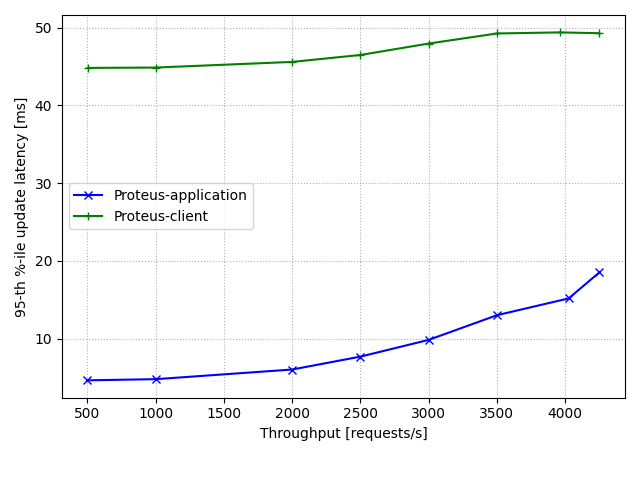
\includegraphics[width=0.7\textwidth]{./figures/evaluation/fr_latency_throughput.png}
  \caption{Throughput vs 95th percentile update latency.}
  \label{fig:fr_latency_throughput}
\end{figure}

Figure~\ref{fig:fr_latency_throughput} shows 95th percentile update latency as throughput increases,
for the Proteus/remote and Proteus/local deployments.
As described above, update latency is the delay between committing a vote in the Lobsters database,
and the corresponding vote count update in the materialized view.
The ideal throughput--update latency curve would be a horizontal line with latency close to the lower bound defined by
the communication latency.
The lower bound for Proteus/remote is 40 ms while for Proteus/local it is less than 1ms.
In reality, latency remains low as long as the system can keep up with the offered vote request load,
and then increases.

Results show the Proteus/local setup scales well; Update latency remains within 5-10 ms of the lower bound.
The Proteus/remote setup exhibits a higher update latency:
For 4250 requests/second, the update latency in Proteus/remote is 88\% higher than in Proteus/local,
relative to the lower bound.
This can be attributed to the same reasons as the scalability difference between the two deployments:
The Materialized view QPU in Proteus/remote is more loaded because more connections are concurrently ongoing
for the same load value, compared to Proteus/local,
leading to increased latency for applying updates to the view.

\begin{figure}[H]
\centering
  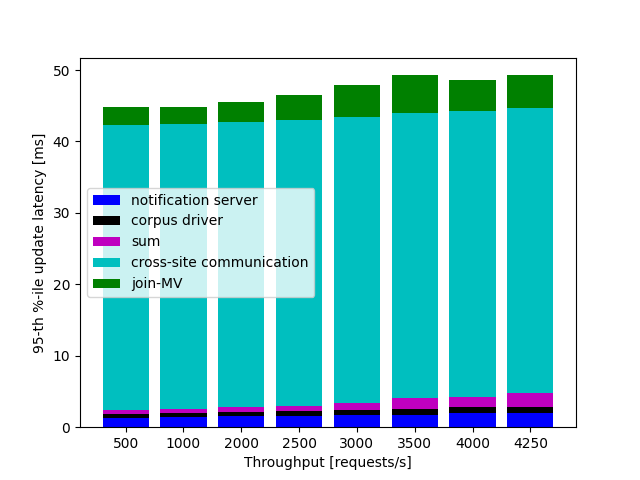
\includegraphics[width=0.7\textwidth]{./figures/evaluation/fr_latency_throughput_breakdown.png}
  \caption{Breakdown of 95th percentile update latency in the Proteus/local deployment
  (as shown in Figure~\ref{fig:fr_latency_throughput}) as throughput increases.}
  \label{fig:fr_latency_throughput_breakdown}
\end{figure}

Each vote committed in the database triggers a record that flows through the QPU graph, and eventually updates the corresponding
vote count in the Materialized view QPU.
Figure~\ref{fig:fr_latency_throughput_breakdown} shows a breakdown of the update latency in the Proteus/local
deployment.
It depicts the delay at each step that vote records follow through the QPU graph.

A vote record's path consists of the following steps:
\begin{enumerate}
  \item When the transaction that inserts a vote record into the Lobsters database commits,
  a trigger sends a message to the notification server (Section~\ref{sec:implementation}).
  The notification server then constructs an update record and sends it to the Corpus Driver QPU through a gRPC stream.
  The duration of this step is shown as \textbf{notification server} in Figure~\ref{fig:fr_latency_throughput_breakdown}.

  \item The Corpus driver receives an update record, and forwards it to the Sum QPU (\textbf{corpus driver}).

  \item The Sum QPU receives an update record, computes an updated vote count,
  and sends a corresponding record to the Join QPU (\textbf{sum}).

  \item \textbf{Cross-site communication} in Figure~\ref{fig:fr_latency_throughput_breakdown} corresponds to the delay for
  sending an update record from the Sum QPU, located at the server site, to the Join QPU, located at the client site.

  \item Finally, the Join QPU receives a record and updates the materialized view accordingly (\textbf{join-MV}).

\end{enumerate}

We observe that:
\begin{itemize}
  \item Update latency is dominated by cross-site communication  (up to 89\%).
  \item Latency at the Corpus driver and Sum QPUs is low: 2ms and 6ms at most.
  This is expected: the Corpus driver simply forwards records upstream;
  The Sum QPU, for each record, updates a vote count stored in memory, and sends a record upstream.
  \item Latency at the notification server and Materialized View QPU increases as the offered load increases.
  However, both scale well as the load increases.
  For the Materialized view QPU this is due to the increasing load in the database that stores the materialized view.
  The latency increase in the notification server can be attributed to the increased load in the database,
  resulting in more triggers being executed concurrently.
\end{itemize}

\begin{figure}[H]
\centering
  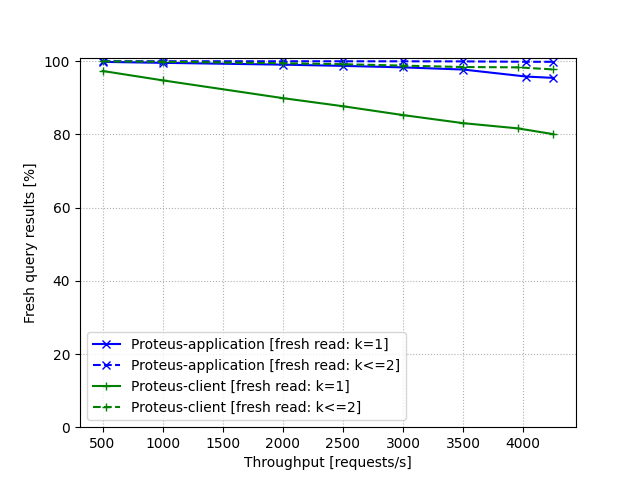
\includegraphics[width=0.7\textwidth]{./figures/evaluation/fresh_reads_throughput.png}
  \caption{Throughput vs percentage of query results and that return a fresh version.
  A returned result is considered fresh if 1) it is the most up-to-date version committed in the database at that time (k=1),
  2) it is amongst the two most up-to-date versions committed in the database at that time (k$\leq$2).}
  \label{fig:fresh_reads_throughput}
\end{figure}

\bigskip
\noindent
Figure~\ref{fig:fresh_reads_throughput} shows the freshness of query results as throughput increases,
measured as the percentage of query results that returned fresh versions.
We define a returned result as a single story with its vote count;
Each front page request returns 25 stories, and each is considered separately.
We consider a scenario in which only the most latest version is considered fresh (k=1),
and one in which the two most recent versions are considered fresh (k$\leq$2).

We observe that:
\begin{itemize}
  \item Proteus/remote has better freshness than Proteus/local, as expected.
  For the k=1 scenario, over 95\% of reads observe the latest versions under the highest load.
  For the k$\leq$2 scenario, freshness remains nearly constant at over 99\%.
  \item Freshness in Proteus/local decreases as throughput increases.
  Proteus/local suffers from up to 80\% stale query results (for k=1), and freshness decreases constantly as load increases.
  However, most stale results observe the second most up-to-date version:
  in the k$\leq$2 scenario over 97\% of query results are fresh.
\end{itemize}

These results can be explained using Figure~\ref{fig:fr_latency_throughput}.
In Proteus/local, it takes at least 45 ms for an updated vote count to be reflected in the materialized view,
but a front page request reaches the view with significantly lower delay.
When load is low, this does not lead to stale query results because there are a few vote requests (5\%).
However, as load increases, queries observe increasingly more stale materialized view  entries.

This is not the case for Proteus/remote.
There, both types of requests reach the materialized view with similar delay,
and because of the query-heavy nature of the workload,
most queries observe tha latest materialized view entries.

\begin{figure}[H]
\centering
  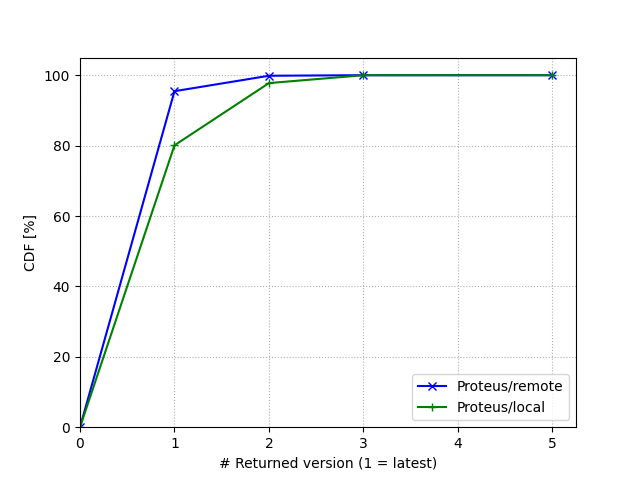
\includegraphics[width=0.7\textwidth]{./figures/evaluation/readV_cdf_throughput.png}
  \caption{CDF of returned version at 4250 requests/second for the Proteus/remote and Proteus/local deployments.}
  \label{fig:readV_cdf_throughput}
\end{figure}

Figure~\ref{fig:readV_cdf_throughput} displays a CDF showing how stale a result of a front page request is
(measured in number of versions),
under a load of 4250 requests/second, for the Proteus/remote and Proteus/local deployments.
Results show that:
\begin{itemize}
  \item In both deployments, most queries return the latest or second most recent version.
  \item Proteus/remote has better freshness than Proteus/local:
  Under the same conditions, Proteus/remote exhibits 4.5\% stale returned results,
  while Proteus/local 20\% (4.4X).
  However, in Proteus/local only 2.2\% of queries results are more stale than the second most recent version.
\end{itemize}

\medskip
\noindent
\textbf{Conclusion.}
Placing the materialized view close to the client, and thus away from the underlying datastore incurs a freshness penalty:
queries return stale results relative to the results that would have been obtained by querying the database.
However, for the workload characteristics in these experiments,
query results are rarely more stale than the second most recent version.
Moreover, update latency and versions freshness scale well as the system's load increases.
We can argue that the level of freshness shown in these experiments to be achievable when placing materialized views close
to the client is sufficient for many query-heavy applications that tolerate eventual consistency.

\subsubsection{Freshness vs round-trip latency}
\label{sec:eval_freshness_rtt}

The experiments in the previous section evaluated the effect of the query processing state placement under a constant
round-trip delay, as the load offered to the system increases.
In this section, we invert these two variables:
we measure freshness under a constant load,
as the (simulated) round-trip time between the application and client site increases,
for the Proteus/local deployment.
The aim of this experiment is to examine the effect of round-trip delay in freshness.

Experiments are performed under a load of 2000 and 4000 requests/second.
We have selected these values based on the results shown in Figure~\ref{fig:fr_latency_throughput}:
Under a load of 2000 requests/second both deployments are able to keep up with the offered load,
while under 4000 requests/second the Proteus/remote scheme exhibits increased update latency.

\begin{figure}[H]
\centering
  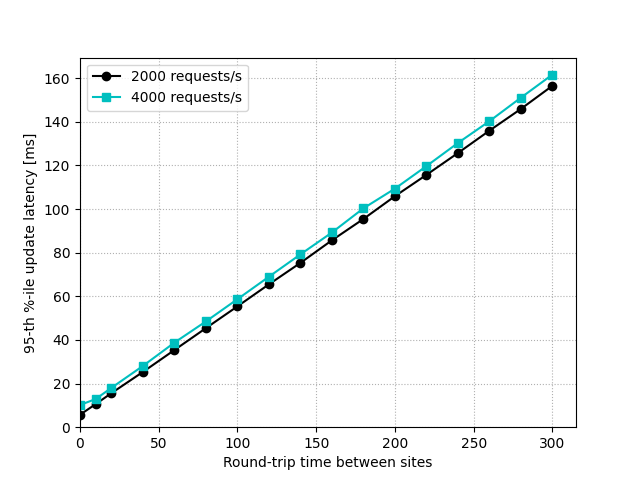
\includegraphics[width=0.7\textwidth]{./figures/evaluation/fr_latency_net_latency.png}
  \caption{Round-trip time between sites vs 95th percentile update latency, for the Proteus/local deployment.}
  \label{fig:fr_latency_net_latency}
\end{figure}

Figure~\ref{fig:fr_latency_net_latency} shows the update latency as the round-trip time between the two sites increases,
under 2000 and 4000 requests/second.
We observe that for both loads, update latency scales linearly with the round-trip time.
Under 2000 requests/second, update latency is at most 5ms above the lower bound set by the one-way network latency
between the two sites, while under 4000 requests/second it is at most 11ms (2.2X).

\begin{figure}[H]
  \begin{subfigure}{0.5\textwidth}
    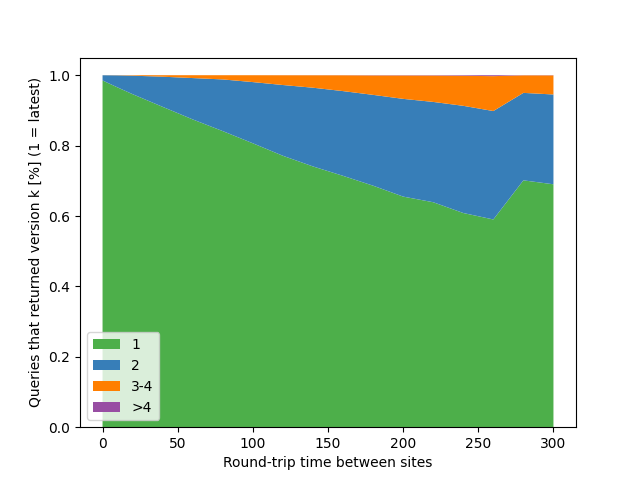
\includegraphics[width=\linewidth]{./figures/evaluation/readV_freshness_netLatency_200.png}
    \caption{2000 requests/second.}
    \label{fig:readV_freshness_netLatency_200}
  \end{subfigure}%
  \hspace*{\fill}
  \begin{subfigure}{0.5\textwidth}
    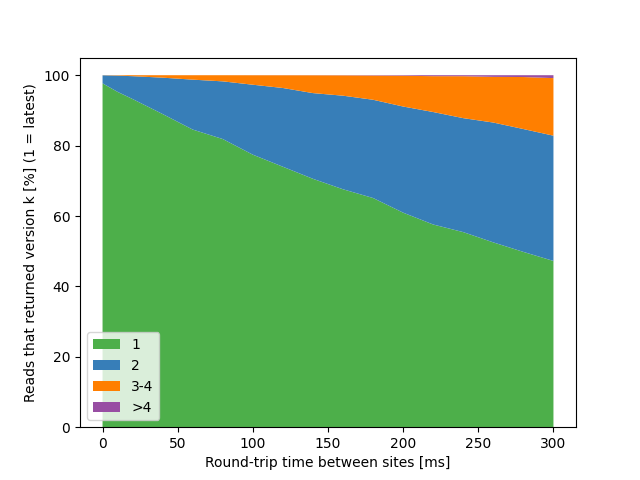
\includegraphics[width=\linewidth]{./figures/evaluation/readV_freshness_netLatency_400.png}
    \caption{4000 requests/second.}
    \label{fig:readV_freshness_netLatency_400}
  \end{subfigure}%
\caption{Distribution of returned version vs round-trip time between sites.}
\label{fig:readV_freshness_netLatency}
\end{figure}

Figures~\ref{fig:readV_freshness_netLatency_200} and~\ref{fig:readV_freshness_netLatency_400}
show the distribution of returned version (which version relative to the most recent one was returned by a query)
for 2000 and 4000 requests/second respectively.
We observe that under both loads freshness decreases as round-trip time increases;
Increasing the load of the system increases the gradient of this decrease.
However, in both cases, queries, generally, observe at most the forth most recent version:
Only 0.06\% and 0.8\% of query results are more stale than the forth most recent version.

\medskip
\noindent
\textbf{Conclusion.}
Update latency, and the freshness of query results are primarily affected by round-trip time between sites,
and to a lesser degree by the system's load.

\subsection{Data transfer between sites}
\label{sec:eval_data_transfer}

\begin{table}[H]
\centering
\begin{tabular}{|c||c|c|c||}
\hline
Deployment & Baseline/remote & Proteus/remote & Proteus/local \\
\hline
Cross-site data transfer (MB) & 0 & 0 & 7.7 \\
\hline
Data transfer out to internet (MB) & $\approx$7700 & $\approx$7700 & $\approx$7700 \\
\hline
\end{tabular}
\caption{Measured data transfer for a 5 minute benchmark with a load of 4000 requests/second.}
\label{tab:data_transfer}
\end{table}

Distributing a query engine across multiple sites entails data transfer between sites.
If the system is deployed on a public cloud platform this incurs an additional cost
because data transfer between data centers is part of public clouds' pricing models.
For example, on AWS EC2, data transfer costs \$0.02 per GB \cite{aws:pricing}.

In the scenario used for these experiments, placing the Materialized view QPU at the client site entails that
update records from the Sum to the Materialized view QPU are sent between sites.

To measure the amount of inter-site data transfer,
we have implemented a mechanism for measuring and aggregating the size of outgoing messages at each QPU.
For a 5 minute benchmark, with 4000 requests/second (200 votes/second), 7.7MB of data were transferred between data centers.
This is because only 5\% of requests are votes, and the size of an update record is small (around 90 bytes),
as it only contains the id and vote count of a story.

In contrast, in the same benchmark, 7.5GB of data were sent as query responses.
This is because the size of a query response is around 4MB
(it contains the records of 25 stories), and 95\% of requests are queries.

We conclude that, in this the evaluation scenario, the materialized view can be placed in the client site without incurring
significant data transfer costs.

\subsection{Conclusion}

The evaluation presented in this section demonstrates that there are benefits and drawbacks to both placement options:
Placing materialized views close to the client results in improvements in response time and throughput,
at the expense of freshness.
Conversely, placing materialized views close to the corpus ensures fresh query results,
but brings limitations to response time and throughput.
As a result, client-site placement of materialized views is more suitable for applications that require low query response times or high
query load, and can tolerate stale query results;
server-site placement is better-suited for applications for which query processing performance is not critical,
but require up-to-date query results.
In addition, evaluation results show that Proteus can to efficiently implement both placement schemes.


\section{Federated metadata search for multi-cloud object storage}
\label{sec:eval_2}

\subsection{Experimental scenario}

The evaluation presented in this section is based on the case study presented in Section~\ref{sec:zenko}.
We consider a multi-cloud data serving system, composed of three storage locations.
A storage location may be a public cloud storage platform (e.g. Amazon S3, Microsoft Azure Blob storage, Google Cloud Storage),
or an on-premise storage system.
Each storage location is independent (not aware of the other locations),
and a multi-cloud data controller (\S\ref{sec:zenko}) is responsible for providing a common namespace across storage locations.
The controller implements an object storage API, such the AWS S3 API:
objects are composed of a primary key, a set of metadata attributes, and content.
This evaluation focuses on providing support for federated queries on metadata attributes.

We consider a system model composed of the 3 storage locations, in 3 geographically distant data
centers.
Each storage location stores a disjoin subset of the dataset.
An instance of the multi-cloud controller is deployed on each storage location,
and users are served by the controller that is geographically closer to their location.
An overview of the system model is shown in Figure~\ref{fig:eval_part2_overview}.

We consider an application that consists of two types of operations:
updating the metadata attributes of a given object,
and performing queries on metadata attributes.

\begin{figure}[H]
\centering
  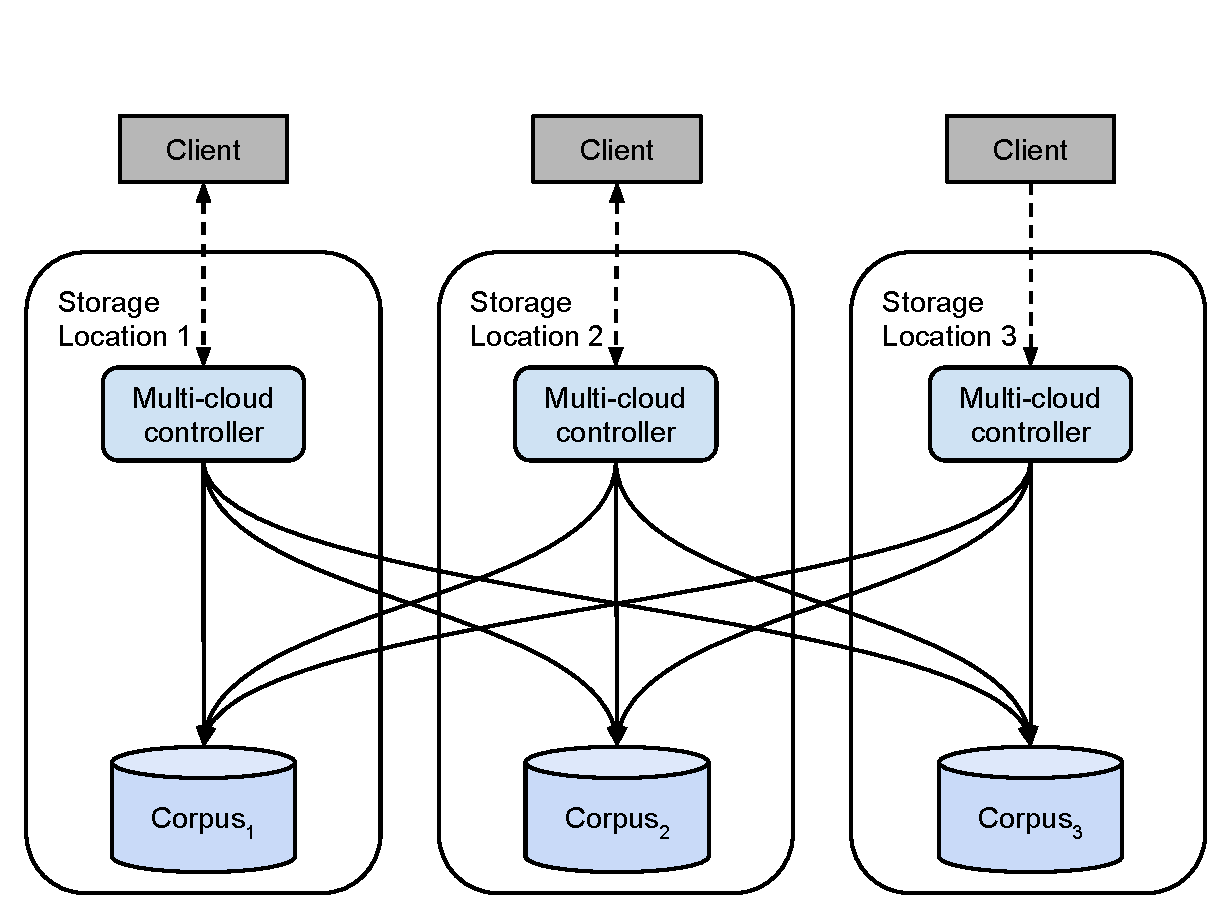
\includegraphics[width=0.7\textwidth]{./figures/evaluation/eval_part2_overview.pdf}
  \caption{An overview of the system model in \S\ref{sec:eval_2}.}
  \label{fig:eval_part2_overview}
\end{figure}

\subsection{Methodology}

As discussed in Section~\ref{sec:zenko}, there are alternative approaches for designing a multi-cloud query engine.
The aim of this evaluation is to demonstrate the need for flexibility in the query engine's design for addressing the
needs of different applications,
and validate that QPU-based query engines can provide the required flexibility.

To achieve that, we consider 3 query engine configurations (QPU graphs), 3 workload types with different query-update ratios,
and 3 metrics (query processing performance, freshness, and data transfer between storage locations);
We experimentally determine which query engine configuration is better-suited for each combination of workload type and target metric.

\bigskip
\noindent
\textbf{Query engine configurations.}
The main functionality of the query engine in this scenario is to maintain secondary indexes for accelerating queries on
metadata attributes.
We consider the following approaches for partitioning and placing a multi-cloud secondary index across the system.

\begin{itemize}
  \item \textbf{Replicated global indexes (rg-index):}
  An index responsible for indexing data from all storage locations is deployed on each location.
  This approach has the advantage that queries are served by the local index.
  However, each index needs to receive update notifications from the two remote storage locations.
  Depicted in Figure~\ref{fig:rg_index}.

  \item \textbf{Partitioned index (p-index):}
  In this configuration, the index on each storage location is responsible for the local corpus.
  The system forwards each query to all 3 storage locations, and combines the retrieved results.
  This approach requires a third of the storage space for indexes compared to rg-index,
  and ensures that update notifications are sent only to the local index,
  at the expense of requiring cross-site communication for serving queries.
  Depicted in Figure~\ref{fig:p_index}.

  \item \textbf{Partitioned index with caching (p-index-cache):}
  This configuration is an extension to p-index that uses a caching layer with the aim of reducing access to remote indexes.
  For each index, a cache responsible for caching sub-query results from it is deployed on the two remote storage locations.
  Depicted in Figure~\ref{fig:p_index_cache}.
\end{itemize}

\begin{figure}[H]
  \begin{subfigure}{0.5\textwidth}
    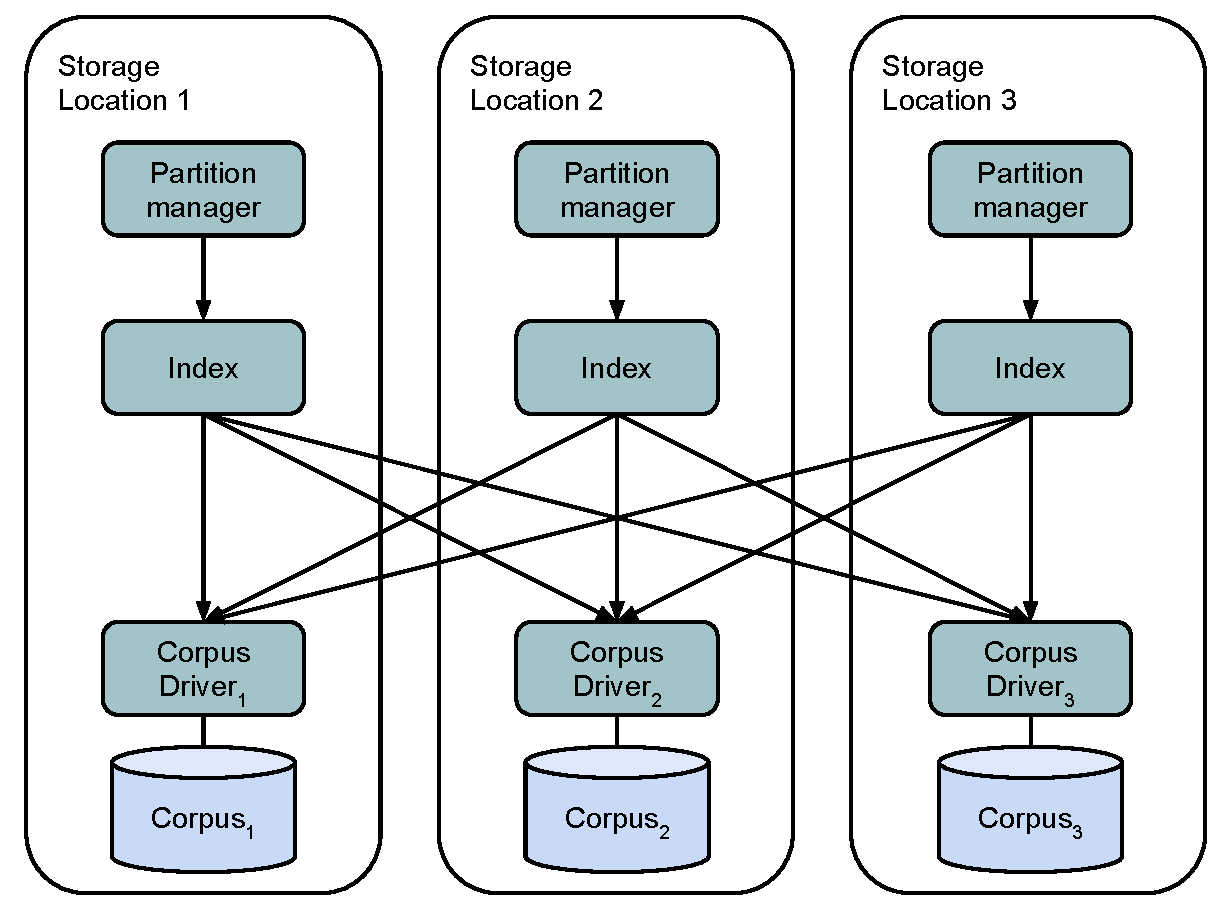
\includegraphics[width=\linewidth]{./figures/evaluation/rg_index.pdf}
    \caption{}
    \label{fig:rg_index}
  \end{subfigure}%
  \hspace*{\fill}
  \begin{subfigure}{0.5\textwidth}
    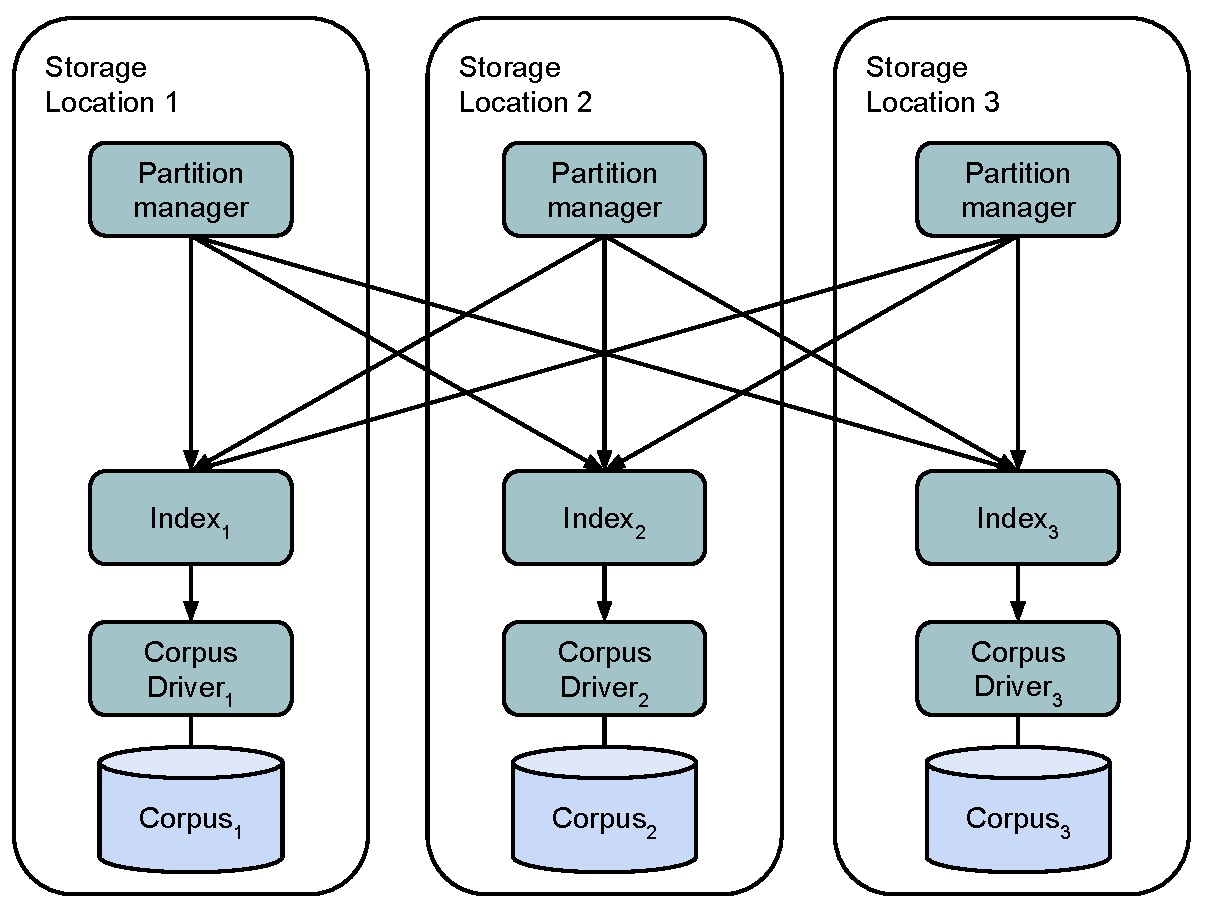
\includegraphics[width=\linewidth]{./figures/evaluation/p_index.pdf}
    \caption{}
    \label{fig:p_index}
  \end{subfigure}%
  \caption{The (a) replicated global indexes (rg-index) and (b) partitioned index (p-index) QPU graph configurations.}
  \label{fig:p_rg_index}
\end{figure}

\begin{figure}[H]
\centering
  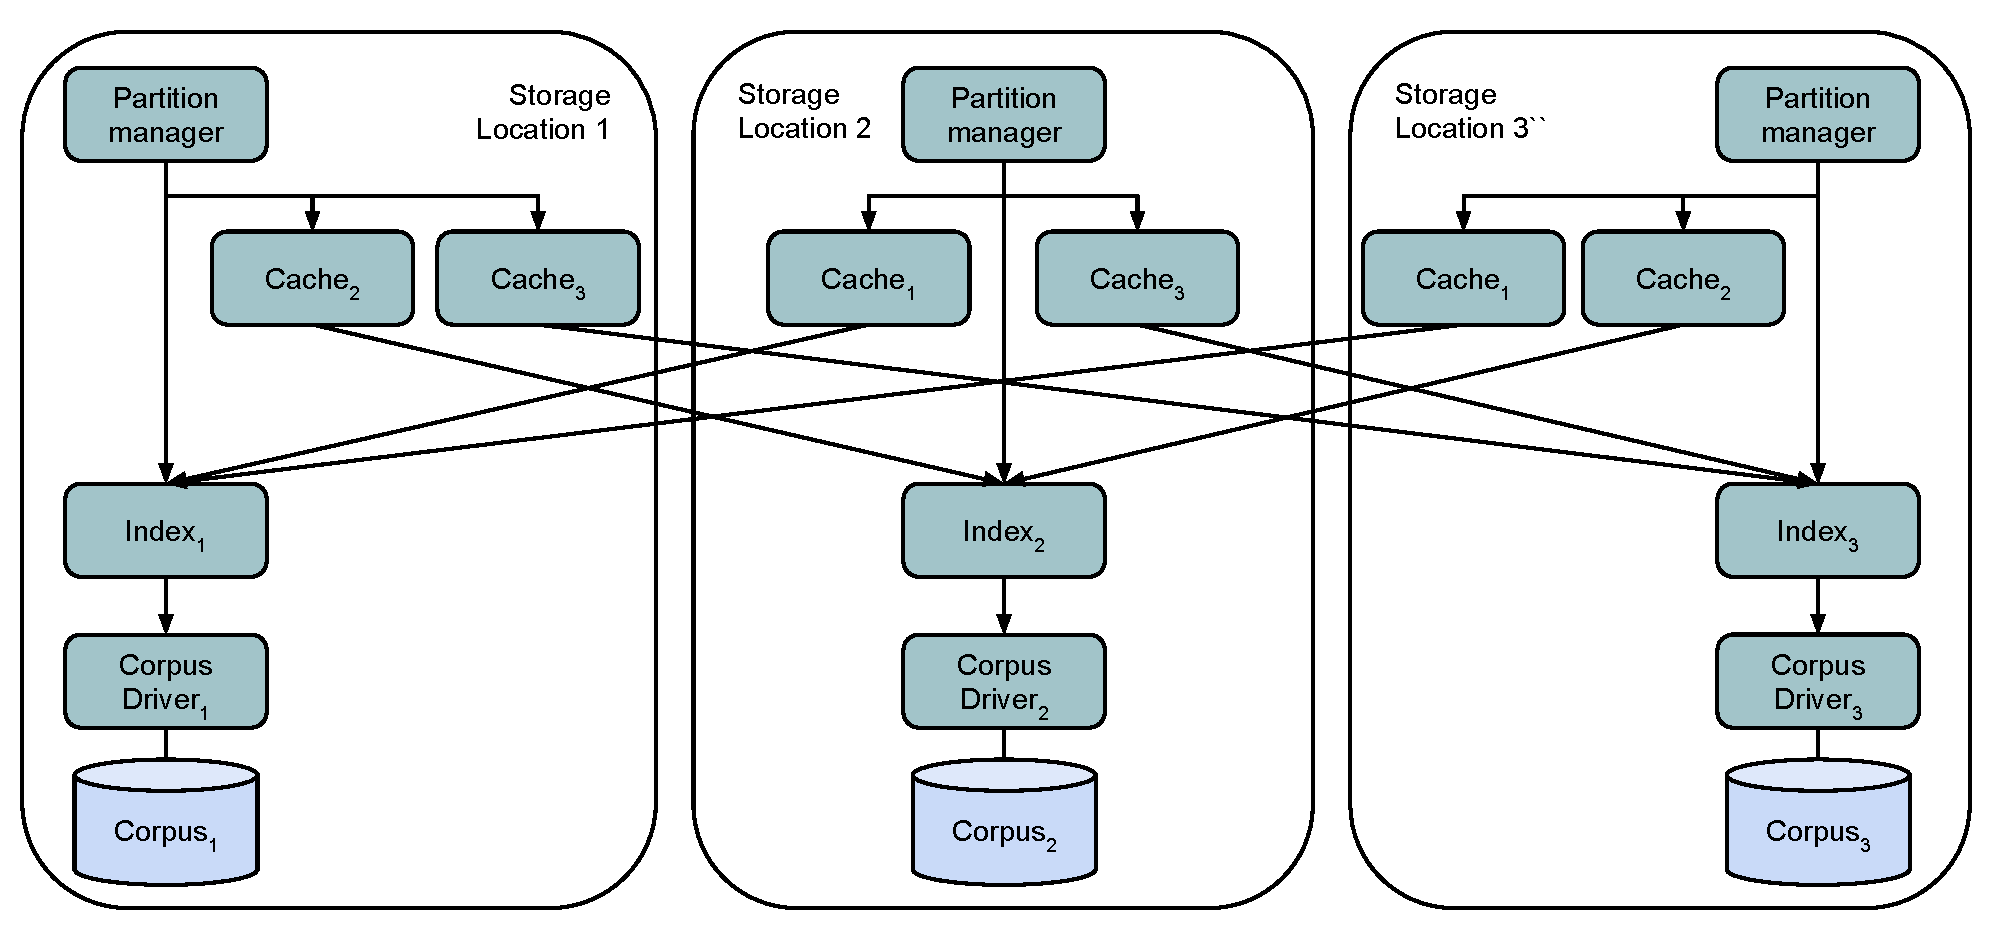
\includegraphics[width=0.7\textwidth]{./figures/evaluation/p_index_cache.pdf}
  \caption{The partitioned index with caching (p-index-cache) QPU graph configuration.}
  \label{fig:p_index_cache}
\end{figure}

\bigskip
\noindent
\textbf{Workload types.}
Overall, we consider a query-heavy application that requires the use of secondary indexes for query processing.
We examine 3 workload types, each with a different mix of query and update operations:
95\% queries - 5\% updates (w95/5), 80\% queries - 20\% update (w80/20),
60\% queries - 40\% update (w60/40).

\bigskip
\noindent
\textbf{Evaluation metrics.}
For this evaluation, we use the metrics discussed in Section~\ref{sec:eval_1}:
query processing performance, freshness and data transfer cost for data transferred between storage locations.

\subsection{Experimental Setup}
On each storage location, data is stored on an instance of MongoDB.
We use MongoDB as an object store:
an object is represented by a MongoDB document, with document fields representing the object's metadata attributes.
At the start of each experiment, we preload each storage location with with 33k objects,
so that in total the system stores 100k objects.

The Index QPU implements an in-memory B-tree secondary index.
The Cache QPU implements a cache with a least recently used (LRU) eviction policy,
and a time-to-live (TTL) based invalidation policy.
We set the size of caches so that each cache can hold 50\% of the index entries it is responsible for,
and configure the TLL value to 5 seconds.

We configure the system so that there is an 80sm round trip time between storage locations in order to
simulate a multi-cloud system deployed over distant geographic locations.

\bigskip
\noindent
\textbf{Workload generation and measurements configuration.}
We use the Yahoo! Cloud Serving Benchmark (YCSB) \cite{ycsb} for generating workload and performing measurements.
The core operation of the YCSB framework is that it drives a number of client threads,
each executing a sequential series of operations by making calls to the underlying system,
and measures the latency and achieved throughput of their operations.
At the end of an experiment, a statistics model aggregates the measurements and reports the achieved throughput and
the measured latency percentiles.

We have modified YCSB's MongoDB driver to send query operations to Proteus.
We deploy a YCSB instance on each storage location.
On each location, YCSB client threads send update operations to the local MongoDB instance,
and query operations to the local Partition Manager QPU.
At the end of an experiment, we gather and aggregate measurements from all three storage locations,
and compute the total achieved throughput and latency percentiles.

Each object in the dataset has multiple, randomly generated metadata attributes.
We ensure that a numeric attribute with a specified key existing in every object.
Query operation in the workload are point queries that refer to this attribute.
Both the attribute's values and query predicated follow a uniform distribution.
We use the mechanism presented in Section \ref{sec:eval_setup} for measuring freshness.

Experiments run for 5 minutes unless otherwise specified, and we start taking measurements after an initial
warmup period of 30 seconds.

\subsection{Query processing performance}

\begin{figure}[H]
\centering
  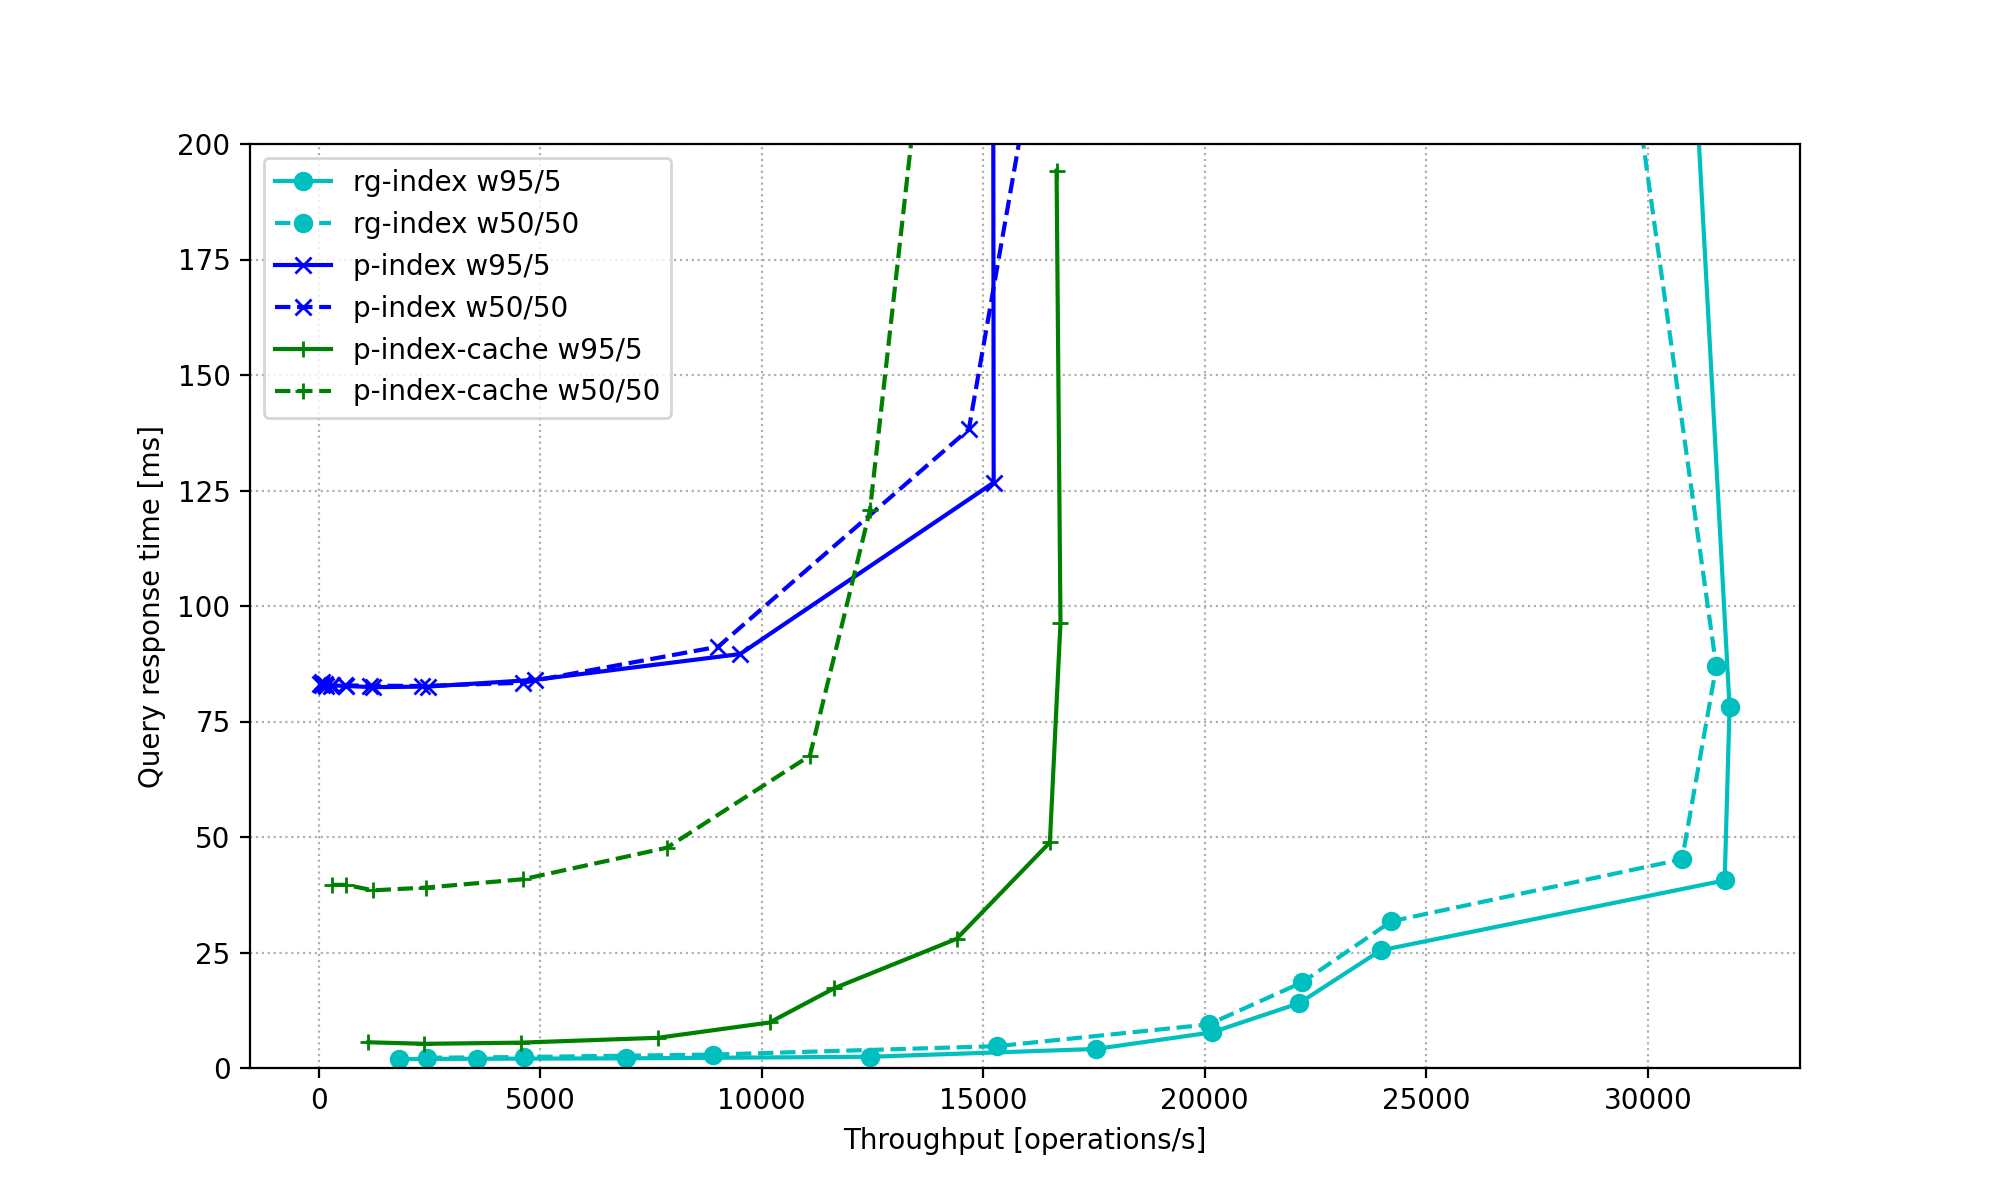
\includegraphics[width=0.9\textwidth]{./figures/evaluation/ycsb_responseTime.png}
  \caption{Throughput vs query response time. Plots for the rg-index and p-index configuration show the 90th percentile response time;
  Plots for the p-index-cache configuration show average response time in order to capture the effect of caching in reponse time.}
  \label{fig:ycsb_responseTime}
\end{figure}

Figure~\ref{fig:ycsb_responseTime} shows throughput--query response time plots for the 3 QPU graph configuration and 3 workload
types.
We observe that:
\begin{itemize}
  \item Response time in the p-index configuration is 80ms higher than in the rg-index configuration.
  This is because in p-index the query engine forwards queries to indexes across storage locations while
  in rg-index queries are served by the local index.
  \item Average response time in the p-index-cache configuration is around 80ms when load is low,
  and then decreases as load increases.
  This effect is the result of caching:
  In low load values, caches are not filled, and most queries result in cache misses;
  As load increases, more queries are served from the cache, decreasing the average query response time.
  \item The p-index configuration achieves around 50\% throughput compared to rg-index.
  This can be attributed to the closed loop workload generation mechanism of YCSB:
  Given a certain number of client threads, in rg-index each query operation has a takes less than 25ms
  when the system is not saturated, while in p-index each query operation take 85-90ms because of the 80ms
  round trip time between storage locations.
  Therefore, in p-index each client thread cannot offer the same load as in rg-index.
  \item The p-index-cache configuration achieves 21\% lower throughput (for the w95/5 workload).
  This is expected as each cache miss adds an 80ms overhead to response time,
  resulting in client threads being able to generate less load.
\end{itemize}

We conclude that the rg-index configuration is better-suited for achieving the best query processing performance.
However, this comes at the expense of memory overhead for maintaining a global index at each storage location.
The rg-index-cache configuration requires achieve query processing performance comparable to rg-index,
and requires 66\% the memory of rg-index (because each cache is configured to 50\% the size of an index).

\subsection{Freshness}

In this section, we examine the query result freshness achieved by the alternative QPU graph configurations.
In order to evaluate the freshness of the different configurations,
we break them down into \textit{placement patterns}, we evaluate the freshness of each placement pattern,
and reason about how placement pattern freshness contributes to the overall freshness of QPU graph configurations.
The placement patterns present in the three QPU graph configurations are shown in Figure~\ref{fig:placement_patterns}.

\begin{figure}[H]
  \begin{subfigure}{0.24\textwidth}
    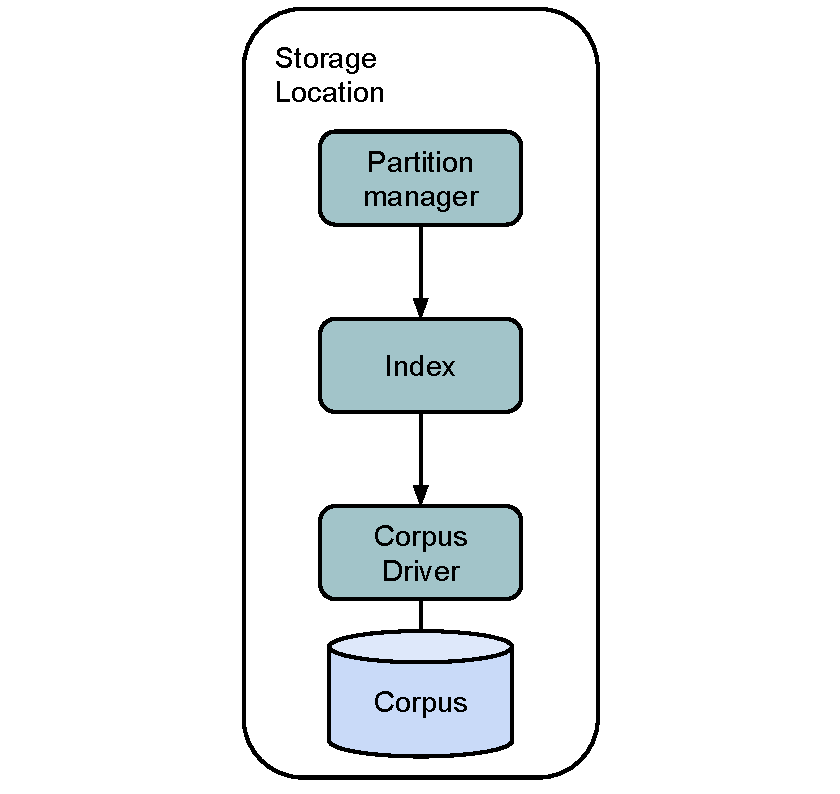
\includegraphics[width=\linewidth]{./figures/evaluation/ycsb_freshness_local.pdf}
    \caption{}
    \label{fig:ycsb_freshness_local}
  \end{subfigure}%
  \hspace*{\fill}
  \begin{subfigure}{0.24\textwidth}
    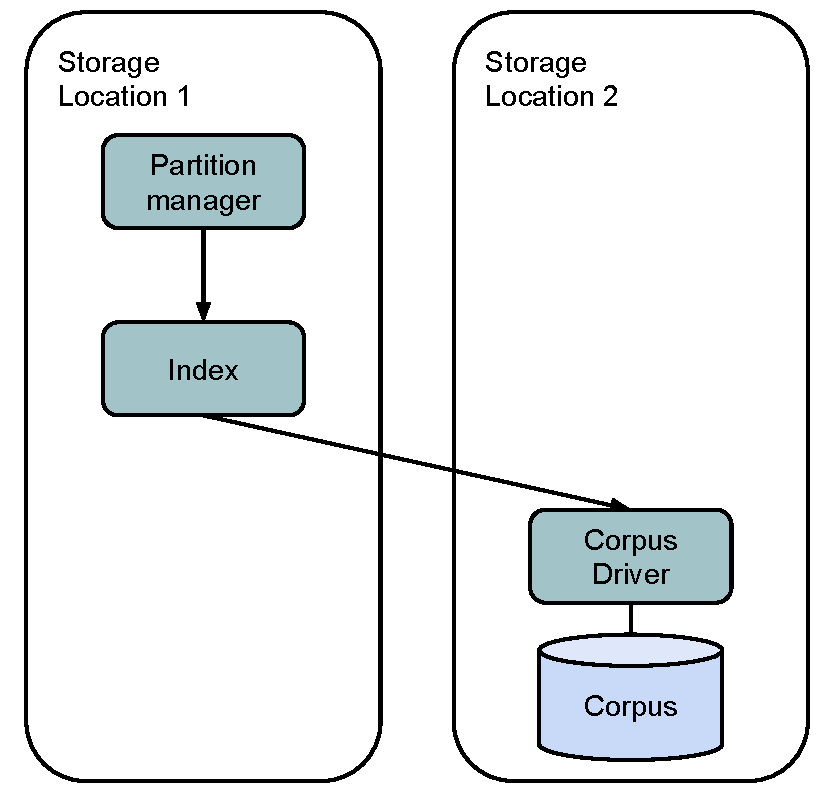
\includegraphics[width=\linewidth]{./figures/evaluation/ycsb_freshness_remote_corpus.pdf}
    \caption{}
    \label{fig:ycsb_freshness_remote_corpus}
  \end{subfigure}%
  \hspace*{\fill}
  \begin{subfigure}{0.24\textwidth}
    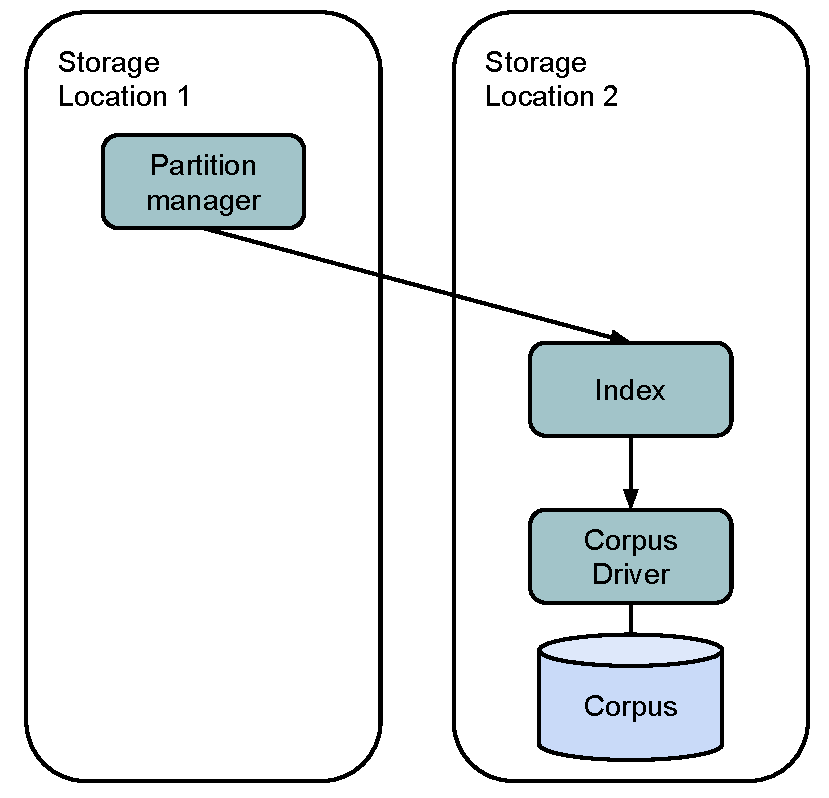
\includegraphics[width=\linewidth]{./figures/evaluation/ycsb_freshness_remote_client.pdf}
    \caption{}
    \label{fig:ycsb_freshness_remote_client}
  \end{subfigure}%
  \hspace*{\fill}
  \begin{subfigure}{0.24\textwidth}
    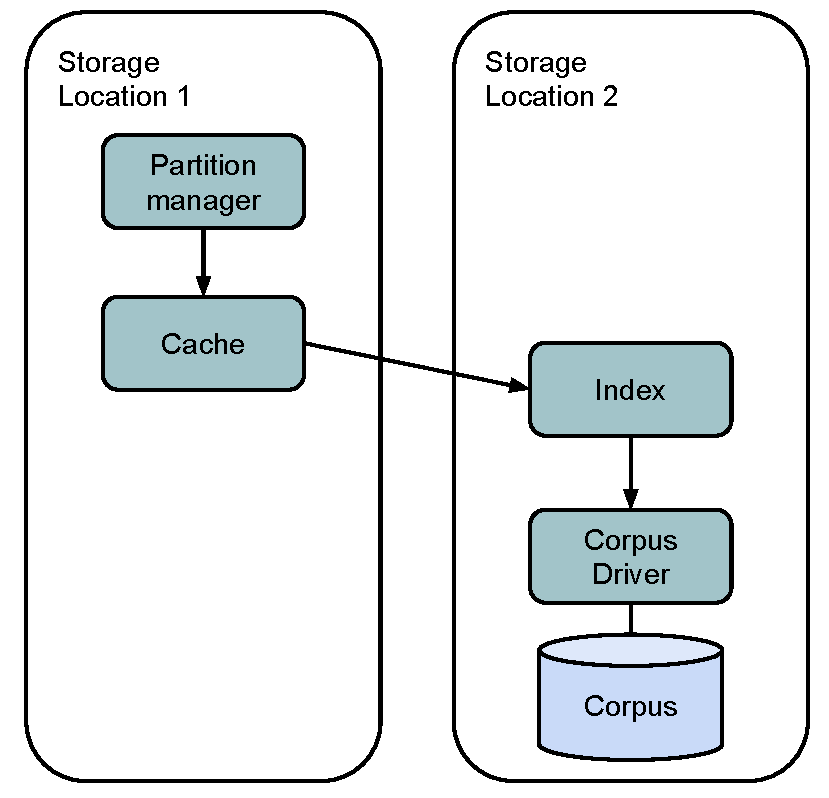
\includegraphics[width=\linewidth]{./figures/evaluation/ycsb_freshness_remote_client_cache.pdf}
    \caption{}
    \label{fig:ycsb_freshness_remote_client_cache}
  \end{subfigure}%
  \caption{Placement patterns. (a) Corpus, index and clients are located on the same storage location (local).
  (b) The corpus is located on a remote storage location (remote-corpus). (c) The index is co-located with the corpus;
  clients are located on a remote storage location (remote-client). (d) A cache is used to reduce cross-location communication (remote-client-cache).}
  \label{fig:placement_patterns}
\end{figure}

\begin{table}[H]
\centering
\begin{tabular}{|c||c|c|c|c||}
\hline
& local & remote-corpus & remote-client & remote-client-cache \\
\hline
rg-index & $\blacksquare$ & $\blacksquare$ &  & \\
\hline
p-index & $\square$ & & $\blacksquare$ & \\
\hline
p-index-cache & $\square$ & &  & $\blacksquare$ \\
\hline
\end{tabular}
\caption{Placement patterns that QPU graph configurations are composed of.
$\blacksquare$ $\blacksquare$ indicates that both patterns contribute to the configuration's freshness.
$\square$ $\blacksquare$ indicated that only the pattern with $\blacksquare$ contributed to the configuration's freshness.}
\label{tab:placement_patterns}
\end{table}

Table \ref{tab:placement_patterns} shows the placement patterns used for each QPU graph configuration.
In rg-index, each index is connected to both local (\ref{fig:ycsb_freshness_local}) and remote (\ref{fig:ycsb_freshness_remote_corpus}) corpus.
As a result, query result freshness is affected by the freshness characteristics of both patterns.
In p-index, each Partition Manager QPU is connected to the the local index (\ref{fig:ycsb_freshness_local}),
and two remote indexes (\ref{fig:ycsb_freshness_remote_client}).
The Partition Manager forwards a given query to all three indexes and waits to receive all responses before responding to
the client.
Because of that, the freshness of p-index is determined by the freshness of the remote-client pattern.
Similarly, the freshness of p-index-cache is determined by the freshness of the remote-client-cache pattern
(\ref{fig:ycsb_freshness_remote_client_cache}).


\begin{figure}[H]
  \begin{subfigure}{0.5\textwidth}
    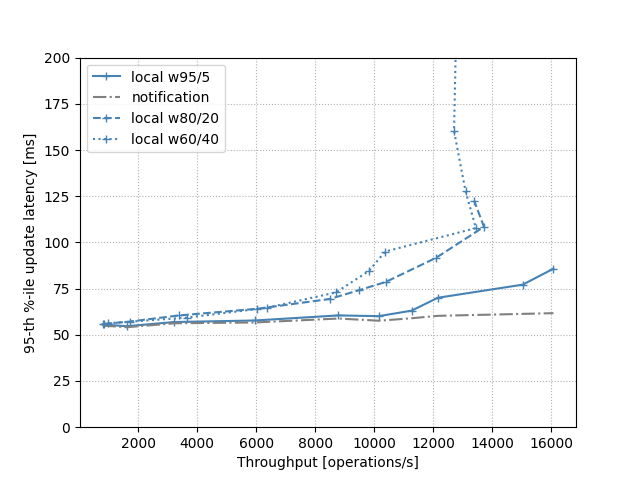
\includegraphics[width=\linewidth]{./figures/evaluation/ycsb_update_latency_local.png}
    \caption{}
    \label{fig:ycsb_update_latency_local}
  \end{subfigure}%
  \hspace*{\fill}
  \begin{subfigure}{0.5\textwidth}
    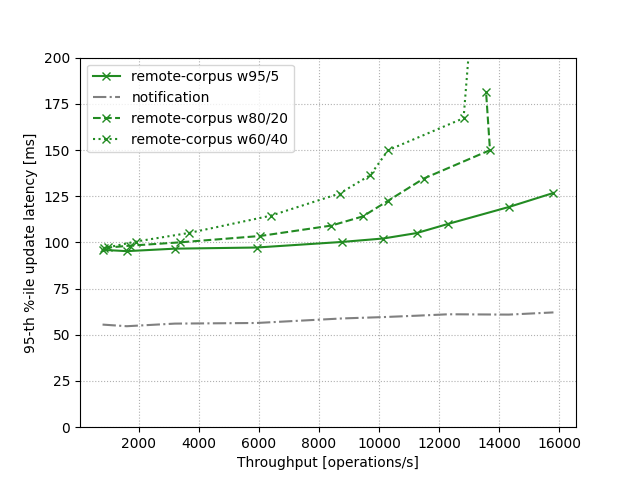
\includegraphics[width=\linewidth]{./figures/evaluation/ycsb_update_latency_remote.png}
    \caption{}
    \label{fig:ycsb_update_latency_remote}
  \end{subfigure}%
  \caption{Throughput vs 95th percentile update latency for the Index QPU in the local (a) and remote-corpus (b) placement patterns.}
  \label{fig:ycsb_update_latency_local_local_remote}
\end{figure}

Figures~\ref{fig:ycsb_update_latency_local} and~\ref{fig:ycsb_update_latency_remote} show the 95th percentile update latency as throughput increases,
for local (\ref{fig:ycsb_update_latency_local}) and remote-corpus (\ref{fig:ycsb_update_latency_remote}) placement patterns.

We implement the storage tier's Subscribe API (\S\ref{sec:storage_tier_api}) using MongDB's change stream functionality \cite{mongo:changestreams}.
Our results show that, with the configuration used for these experiments, the change stream client receives a notification with a 50-60ms delay.
We indicate this as the baseline update latency in the plots (notification).

In addition, we note that our mechanism for measuring update latency includes in update latency
the response time of the update operation performed by the client.
Because update operation response time increases with load, part of the increase in update latency is due to the update operation response time.
Update operation response time is shown in Figure~\ref{fig:ycsb_write_latency}.

\begin{figure}[H]
\centering
  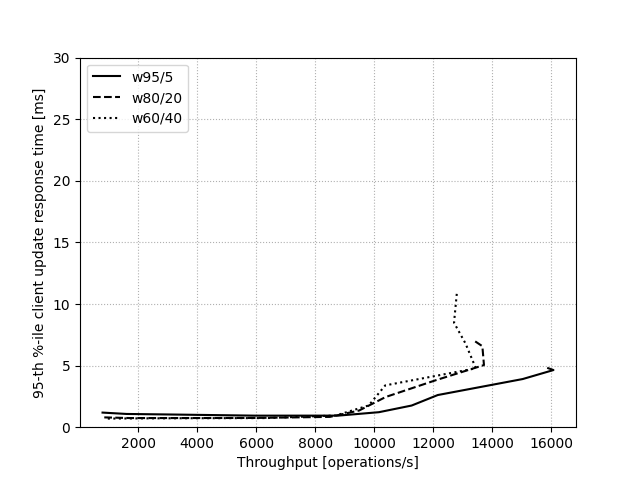
\includegraphics[width=0.7\textwidth]{./figures/evaluation/ycsb_write_latency.png}
  \caption{Throughput vs client update response time. Client updates are always local,
  as in all configurations clients write to the local MongoDB instance.}
  \label{fig:ycsb_write_latency}
\end{figure}

\noindent
For the update latency results in Fig.~\ref{fig:ycsb_update_latency_local_local_remote}, we observe that:
\begin{itemize}
  \item In remote-corpus, update latency is at least 40ms higher that the baseline
  due to the 40ms network latency between storage locations.

  \item Update latency increases with the ratio of updates.
  This is due to contention, as each update needs to acquire a write lock on the index.
  For both placement patterns, for the w80/20 and w60/40 workloads,
  update latency does not scale to loads larger than 13k operations/second.
\end{itemize}

The evaluation results shown in Figures~\ref{fig:ycsb_responseTime} and~\ref{fig:ycsb_update_latency_local_local_remote} demonstrate the trade-off betwee
query performance and query result freshness.
The rg-index configuration, in which queries are served locally, achieves better query processing performance at the expense of increased update latency;
The update latency overhead is determined by the network communication latency between storage locations.
Conversely, the p-index configuration ensures low update latency at the expense query processing performance.
\begin{figure}[H]
  \begin{subfigure}{0.5\textwidth}
    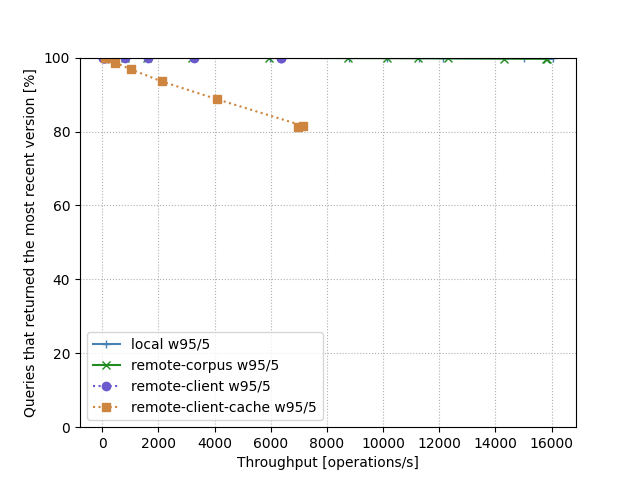
\includegraphics[width=\linewidth]{./figures/evaluation/ycsb_readV_freshness_throughput_9505.png}
    \caption{}
    \label{fig:ycsb_readV_freshness_throughput_9505}
  \end{subfigure}%
  \hspace*{\fill}
  \begin{subfigure}{0.5\textwidth}
    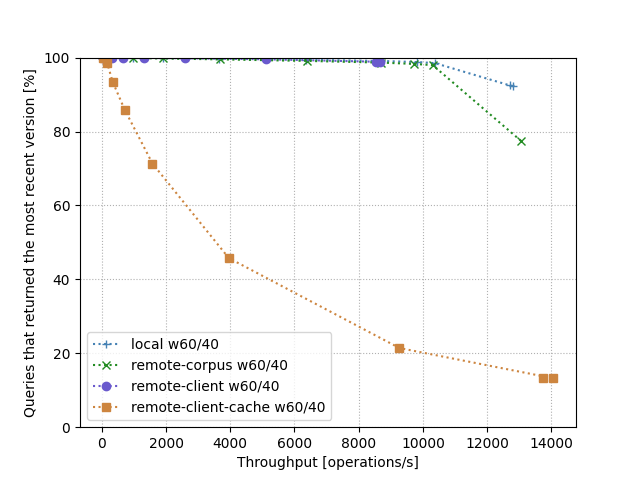
\includegraphics[width=\linewidth]{./figures/evaluation/ycsb_readV_freshness_throughput_6040.png}
    \caption{}
    \label{fig:ycsb_readV_freshness_throughput_6040}
  \end{subfigure}%
  \caption{Throughput vs percentage of queries that returned the most recent version in the w95/5 (a) and w60/40 (b) workload.}
  \label{fig:ycsb_readV_freshness_throughput}
\end{figure}

Next, we examine how update latency affects query result freshness.
Figures~\ref{fig:ycsb_readV_freshness_throughput_9505} and~\ref{fig:ycsb_readV_freshness_throughput_9505} show
the percentage of query operations that return the most recent version of an object as load increases,
for the w95/5 and w60/40 workloads respectively.
We observe that:
\begin{itemize}
  \item For the w95/5 workload, all patterns except remote-client-cache return fresh result for close to 100\% of queries.

  \item For the w60/40 workload, local and remote-corpus return stale results for loads greater than 10k operations/second
  (8\% and 23\% stale query results respectively).

  \item For both workloads, the remote-client-cache pattern results in significantly more stale query results than the other
  patters.
  This is due to the time-based invalidation policy, and the TTL value of 5 seconds.
\end{itemize}

We conclude that, for query-dominated workloads, all pattern exhibit high freshness.
For workloads with higher update rations,
caching with time-based invalidation offers a balance between memory resource overhead and query processing performance,
at the expense of lower query result freshness.

\subsection{Data transfer between storage locations}

\begin{table}[H]
\centering
\begin{tabular}{|c||c|c|c|c||}
\hline
& \textbf{w95/5} & \textbf{w80/20} & \textbf{w60/40} & \textbf{w5/95}\\
\hline
\textbf{rg-index} & 64MB & 213MB & 467MB & 1.37GB \\
\hline
\textbf{p-index} & 18GB & 5.95GB & 5.85GB & 1.25GB \\
\hline
\textbf{p-index-cache} & 4.95GB & 5.58GB & 4.97GB & 947MB \\
\hline
\end{tabular}
\caption{Amount of data transfer between sites for a 5 minute benchmark with 256 YCSB client treads at each storage location.}
\label{tab:ycsb_data_transfer}
\end{table}

In this section, we measure the amount of data sent across storage location for different QPU graph configurations and
workload types.

In the rg-index configuration, cross-location data transfer occurs for sending update notifications from the corpus
to remote Index QPUs:
Each update operation generates three update notifications, one for each storage location.
As a result, data transfer increases as update ratio increases.

In the p-index configuration, cross-location data transfer occurs for retrieving query results from remote Index QPUs.
Partition Manager QPUs forward every query to all three storage locations, and retrieve the results.
As a result, data transfer decreases as query ratio decreases.

In the p-index-cache configuration, cross-location data transfer occurs on cache misses.
When an index entry is not present in a cache, the Cache QPU forwards it to the corresponding Index QPU, and retrieves the
results.
Similarly to the case of p-index, data transfer decreases as query ratio decreases.

These results demonstrate another aspect of the trade-off between the rg-index and p-index configurations.
In general, p-index results in significantly higher data transfer than rg-index.
Our results show that the rg-index configuration results in more data transfer than the p-index configuration for workloads with at least 95\% updates (w5/95).
This because the size of an update notification is significantly smaller than the size of a query response.
Given an update, the update notification contains the object's primary key, the updated attribute(s) and a timestamp;
Given a query, the response contains the primary keys, attributes and timestamps of all objects that match the query predicate.

Furthermore, we observe that using a caching layer results in a 72\% data transfer reduction for the w95/5 workload.
Therefore, using the p-index-cache configuration can result in significant data transfer cost reduction compared to
the p-index configuration.

\subsection{Conclusion}

\begin{table}[H]
\centering
\begin{tabular}{|c||c|c|c||}
\hline
& \textbf{w95/5} & \textbf{w80/20} & \textbf{w60/40}\\
\hline
\textbf{Query processing performance} & rg-index & rg-index & rg-index \\
\hline
\textbf{Query result freshness} & p-index & p-index & p-index \\
\hline
\textbf{Data transfer cost} & rg-index & rg-index & rg-index \\
\hline
\end{tabular}
\caption{Summary of experimental comparison between the three QPU graph configurations.}
\label{tab:ycsb_summary}
\end{table}

Table~\ref{tab:ycsb_summary} summarizes the evaluation results presented in this section
by showing which QPU graph configuration is better-suited for each combination of target metric
and workload type.

However, applications are rarely interested in optimizing a single metric,
but rather finding the right balance in the trade-offs between metrics.
Our evaluation results indicate that, for query heavy workloads,
the p-index-cache configuration offers a balance between query processing performance,
freshness, and memory resource and data transfer overhead.

The evaluation presented in this section demonstrates the trade-offs between
different index and cache partitioning and placement approaches,
and shows that Proteus can be efficiently used to tune the trade-offs between query processing
performance, freshness and operational costs by controlling the query engine's architecture.

\section{Conclusions}

The evaluation results presented in this chapter confirm our analysis of the trade-offs
involved in the placement of derived state.
This validates the central argument of this thesis:
No single derived state partitioning and placement approach is optimal for all needs,
and flexibility is required for addressing different needs.

Moreover, the evaluation demonstrates the expressiveness of the proposed approach:
QPU-based query engines enable the flexibility for configuring derived state partitioning and placement
with simple configuration changes to the query processing middleware, without requiring changes to the application.
QPU-based query engines can be used to flexibly partition derived state, and place state and query processing computation
freely across the system.
THanks to that they can be employed to address diverse application characteristics and requirements.


\chapter{Related work}
\label{ch:related_work}
\section{Secondary attribute querying in non-relational data stores}

%  get intro from SLIK
Many large-scale key-value storage systems sacrifice features like secondary indexing and/or consistency in favor of scalability or performance. This limits the ease and efficiency of application development on such systems.

\subsection{Secondary index based approaches}
A number of implemented secondary indexing approaches for distributed databases have been proposed.

% // SLIK: Scalable Low-Latency Indexes for a Key-Value Store

SLIK \cite{kejriwal:slik} proposes an approach for implementing secondary indexes in a large-scale main key-value store.
It is designed with the goals of low latency, high scalability, consistency
(specifically the requirement of providing the same strong consistency as a centralized system) and high availability.

SLIK partitions secondary indexes using the scheme which we refer to as partitioning by term.

Index partition (referred to as an indexlets) are implemented using B+trees.
Index entries store hashes of data items' primary keys.
Therefore, after an index lookup each data item contains the result need to be retrieved from the storage engine.

To achieve consistent index lookups SLIK
Ordered writes.
Index entries are created before updates to the corresponding data items are applied,
and old index entries are removed asynchronously.
This guarantees that if a data item contains a secondary attribute value, then an index lookup for that value will return the data item,
by ensuring that the lifespan of each index entry spans that of the corresponding data item.

Treating data items as ground truth and index entries as hints.
The system verifies the results of index lookups by checking the corresponding data items.
This guarantees that if a data item is returned by an index lookup then this data item contains the requested secondary key.

Moreover, SLIK performs long-running bulk operations such as index creation, deletion and migration in the background,
n order to avoid blocking blocking normal operations.

SLIK is implemented in RAMCloud \cite{ousterhout:ramcloud}, a distributed in-memory key-value storage system.

This work analyses alternative approaches available in a number of aspects in the design of a secondary indexing system, and discusses the tradeoffs these approaches.
They make specific design decisions guided by their design goals, for example the requirement for consistency for index lookups.
Moreover, this work does not consider a geo-distributed setting.

% // Secondary Indexing Techniques for Key-Value Stores: Two Rings To Rule Them All

\cite{dsilva:tworings}
We have discussed the results of this analysis in detail in section

In this paper, we explore the challenges associated with indexing modern distributed table-based data stores and investigate two secondary index approaches which we have integrated within HBase.
Our detailed analysis and experimental results prove the benefits of both the approaches.
Further, we demonstrate that such secondary index implementation decisions cannot be made in isolation of the data distribution and that different indexing approaches can cater to different needs.
We discuss two indexing strategies for distributed key-value stores:
one based on distributed tables that is able to exploit the table model of the underlying system for index management,
the other using a co-location approach allowing for efficient main-memory access

Both strategies are implemented and integrated into HBase in a non-intrusive way.
We provide an enhanced client interface to query HBase tables using secondary indexing that supports both point queries and range queries.
We present a detailed performance metrics on various database operations with secondary indices and a comparative analysis of the different approaches
We present a thorough analysis on the effects of data distribution on different indexing approaches.
We provided a very detailed analysis of how different data distributions warrant different indexing approaches and demonstrated a case for both implementations.
Our results show that there is clearly a benefit to  having  secondary  indices  in  HBase,and  that  they  can  be  often  built  with  reasonable  performance overhead.
Although there has been some prior works to achieve secondary indexing in HBase,
our work have been more detailed and insightful about the various alternatives and clearly shows that there is no one-stop solution to secondary indexing needs in HBase.



% // Diff-Index: Differentiated Index in Distributed Log-Structured Data Stores
\cite{tan:diffindex}

% // Schema-Agnostic Indexing with Azure DocumentDB
\cite{shukla:schemaagnostic}


% \subsection{Secondary index partitioning schemes}
% \cite{dsilva:tworings}

% \cite{kejriwal:slik}
% SLIK achieves high scalability by distributing index entries independently from their objects rather than co-locating them

% % SLIK: Cassandra [20], DynamoDB [3] and Phoenix [7] on HBase [4] provide local secondary indexes which are partitioned using the co-location approach
% % Some of the systems above like DynamoDB [3] and Phoenix [7] on HBase [4] also provide global secondary indexes, but they are only eventually consistent.

% \subsection{Approaches not based on secondary indexing}

% \textbf{HyperDex: A Distributed, Searchable Key-Value Store} \cite{escriva:hyperdex}

% SLIK =>
% HyperDex is a disk-based large-scale storage system that supports consistent indexing.
% It partitions data using a novel hyperspace hashing scheme by mapping objects’ attributes into a multi-dimensional space.
% As the number of attributes increase, the number of hyperspaces increases dramatically.
% HyperDex alleviates this by partitioning tables with many attributes into multiple lower-dimensional hyperspaces called subspaces.
% HyperDex also replicates the entire contents of objects in each index.
% This means that while HyperDex provides an efficient mechanism for search, it uses more storage space for the extra copies of objects.
% While this is acceptable for disk based systems, it would be very expensive for main-memory based systems.

% \textbf{Replex: A Scalable, Highly Available Multi-Index DataStore} \cite{tai:replex}


% \section{Multi-site Web search}

% \textbf{On the Feasibility of Multi-Site Web Search Engines} \cite{baezayates:multisitefeasibility}

% \textbf{Quantifying Performance and Quality Gains in Distributed Web Search Engines} \cite{cambazoglu:multisitequantifying}

% \textbf{Query Forwarding inGeographically Distributed Search Engines} \cite{cambazoglu:multisiteforwarding}

% \textbf{Improving the Efficiency of Multi-site Web Search Engines} \cite{frances:multisiteimprovingefficiency}

\section{Modular - Flexible architectures}

% // The Click Modular Router


Click \cite{kohler:click} proposes a software architecture for building flexible and configurable routers.

A Click router is assembled from packet processing modules called elements.
Individual elements implement simple router functions like packet classification, queueing, scheduling, and interfacing with network devices.
A router configuration is a directed graph with elements at the vertices;
packets flow along the edges of the graph.
Several features make individual elements more powerful and complex configurations easier to write, including pull connections,
which model packet flow driven by transmitting hardware devices, and flow-based router context, which helps an element locate other interesting elements.

This paper presents Click, a flexible, modular software architecture for creating routers.
Click routers are built from fine-grained components;
this supports fine-grained extensions throughout the forwarding path.
The components are packet processing modules called elements.

A Click element represents a unit of router processing.
An element represents a conceptually simple computation,such as decrementing an IP packet’s time-to-live field,
rather than a large, complex computation, such as IP routing.
A Click router configuration is a directed graph with elements at the vertices.
An edge, or connection, between two elements represents a possible path for packet transfer.

% \bibliographystyle{plainnat}
% \bibliography{refs}

% \section{Distributed query processing}

% \subsection{Query processing in Peer-to-Peer systems}
% DHT stuff.

% \subsection{Query processing in distributed databases}


% \section{Stream processing and Data-flow systems}

\section{Multi-site web search engines}
A series of papers \cite{cambazoglu:multisitequantifying, yates:multisitefeasibility, cambazoglu:multisiteforwarding, frances:multisiteefficiency, kayaaslan:multisitereplication}
has studied the problem of designing a large-scale web search engine architecture over multiple, geographically distributed data centers.

This works consider the following system model:
The search engine architecture is composed of multiple data centers; Data centers are associated with geographical regions.
Each data center stores and crawls and documents that are served by the web sites in its geographical region.
As a result, each data center is responsible for a disjoint subset of the Web.
The search engine builds an inverted index over the crawled documents, which is used to serve queries.

\medskip
\noindent
In \cite{cambazoglu:multisitequantifying}, Cambazoglu et al. a taxonomy of search engine architectures for this problem.
In a \textit{centralized} architecture, the entire index is stored in one, central site,
and all user queries are submitted to this site.

In this architecture, the index might be replicated or partitioned with the site.
This architecture was used by early web search engines as well as small-scale engines.
In \textit{replicated} architecture, the entire index is replicated over multiple data centers.
Queries are routed to data centers based on geographical proximity of users to data centers.
Documents are ranked based on ranking function; the result of query consists of the k highly ranked documents for that
query.

Finally, in a \textit{partitioned} architecture the document collection is partitioned into smaller, non-overlapping
sub-collections such that each data center is responsible for a different sub-collection.
Queries originating in a particular region, are evaluated over the partial index in the corresponding search site.
The underlying assumption in this approach is that users are interested more in documents located in their own region,
and local documents are more relevant for queries originating from the same region.
This leads to gains in query processing time and throughput, as queries are now evaluated over small subsets of
the index.
The downside of this approach is that documents that are relevant to a query but are not local to the search site are
not retrieved, leading to inferior search quality.
The problem of accessing non-local documents has two immediate solutions:
taking the data to where it is sought and/or taking the queries to what they seek.
The first is an offline solution that requires partial replication of the popular documents in a region on some non-local search sites.
The second is an online solution that requires selective forwarding of queries between search sites to extend cover- age of search results.
forwarding of queries between search sites to extend cover- age of search results.

This problem bares similarities to the problem studies in this thesis ...
There are however two significant differences

\medskip
\noindent
The works in \cite{yates:multisitefeasibility} and \cite{cambazoglu:multisiteforwarding}
have proposed techniques for selective query forwarding.
Selective forwarding works as follows:
When a search site receives a query, it estimates the quality of the locally computed results relative to globally computed results
(results that which would have been obtained through evaluation over the full index).
If it is determined that the local index misses some documents that would have appeared in the global ranking,
the local site estimates which remote sites might have those documents, and forwards the query to those sites.
Finally, non-local and local results are merged and returned to the user.

In addition, \cite{cambazoglu:multisiteforwarding} evaluates the impact of result caching
on the rate of locally processed queries.
Results show that with result caching, the fraction of queries that can be locally processed inc increases by 35\% to 45\%.

\medskip
\noindent
In \cite{frances:multisiteefficiency} Kayaaslan et al.
propose strategies for selectively replicating documents across search engine sites.
The key idea is to identify documents that are of interest to the users of certain geographical regions,
based on the occurrence frequencies of documents in past search results,
and then replicate identified documents on remote sites so that future queries can be processed without the need for
forwarding.
Documents replication leads to improvements in the query processing efficiency, as when performed effectively,
fewer queries need to be forwarded, this reducing average query response times and the overall query workload of the search engine.
At the same time, increasing the volume of replicated documents has a negative impact on query processing times of local data centers,
due to the increase in their index sizes.
There is thus a trade-off between replication and search performance.
The work in \cite{kayaaslan:multisitereplication}
proposes three different document replication strategies, each optimizing a different objective:
reducing the potential search quality loss, the average query response time, or the total query workload of the search system.



\section{Result caching}

In \cite{cambazoglu:yahoorefreshing} Cambazoglu et al. present the design of the result cache used
in the Yahoo! search engine.
The authors argue that eviction policies are not critical in the setting of search engines, as those engines ca use
in production large caches by using disk space to store query results.
Instead, this work focuses on the problem of keeping cached results consistent with the search engine’s index
as new batches of crawled documents are indexed.
It proposes a TTL-based strategy for expiring cache entries
and refreshing them by issuing refresh queries,
and presents and algorithm for prioritizing cache entries to be refreshed based on the access frequency of entries and
the age of the cached entry.

In general, we can categorize cache invalidation and approaches in two types.
Coupled or ``push-based'' approaches provide the cache with information about changes to the underlying data
(the web search index in this case).
Decoupled approaches invalidate cached entries without any concrete knowledge of changes to the underlying data.
This work presents a decoupled, ``pull-based'' approach in which the caching system refreshes cache entries by querying
the underlying index.
Our design enables both push- and pull-based cache invalidation and refreshing,
and enables system operators to select approach that is better suited for each particular use case.


% % We show that flushing the cache is not efficient and propose a TTL-based strategy to expire cache entries.

% % we focus on result caches, which store previously computed query results
% % Given the high volume of user queries,
% % result caches emerge as crucial performance components to reduce the query traffic to back-end servers and also to reduce
% % the average query processing latency.

% % One major drawback of large result caches is freshness. Search engine indexes change frequently due to

% This cache introduces the concept of refreshing cache entries and presents a practical algorithm for prioritizing entries to refresh.


% There are two possible approaches for cache invalidation in this context: coupled and decoupled.
% The coupled approach is the one of providing the cache with information about changes to the index.
% This approach is difficult to realize in practice due to the complexity and computational cost of accurately determining changes to the index and propagating them to the result cache.
% Such coupled solutions are out of the scope of this work.

% which we adopt in this work, is the one of invalidating cached entries without any concrete knowledge of changes to the index.
% A simple way to achieve this goal is to use a time-to-live (TTL) value and mark entries as expired once they have been in the cache for longer than TTL.

% mechanism for expiring cache entries based on a time-to-live value and a mechanism for maintaining the cache content fresh
% by issuing refresh queries to back-end search clusters,
% propose a novel algorithm for prioritizing cache entries to be refreshed based on the access frequency of entries and the age of the cached entry.

% examine result caching, and

% % [On the Feasibility of Multi-Site Web Search Engines]
% % contributions
% %  propose such a model to assess the operational costs of multi-site Web search systems.
% % query-processing algorithm that maximizes the amount of queries answered locally, without sacrificing the quality of the results compared to a centralized search engine.

% % assess the feasibility of distributed Web search engines comprising geographically dispersed sites
% % propose a detailed cost model that includes operational costs, and enables us to answer questions
% % - Given  an  optimization  that  reduces  the  average  latency  of an operation (crawling, receiving request, query processing)
% %   how does it affect power consumption?
% % - Given  different local  rates  for  power,  how  much  resource savings are necessary to compensate for such differences?
% % Query-processing algorithm
% % #1, offline index construction : each site builds index on the set of docs assigned to it (local+global)
% %   computes upper bound on the scoring function - threshold -  for each term of docs in a site of local docs: upper bound to the contribution of term t to ranking function for query that contains t
% %   subset of "good-quality" docs replicated and indexed in all sites
% % #2, offline propagation: all sites communicate with each other, exchange thresholds computed at phase #1 -  each site acquires complete info about thresholds of all terms in all sites
% % phase #3, online query processing:
% % each site handles queries it receives: compute matching set of docs from local index, rank them → use thresholds of other sites to decide whether computed results would have been identical to centralized system results
% % use thresholds to obtain guarantees on the quality of partial results computed locally
% % if quality guarantees not satisfied → propagate query to other sites to obtain partial results

% % [Quantifying Performance and Quality Gains in Distributed Web Search Engines]
% % Taxonomy
% % centralized architecture: the entire Web index is stored in one, central site. The index is replicated locally over multiple search clusters located within the site.All user queries are submitted to this single site, where eachquery is completely processed by an individual cluste
% % index replication: The entire index is replicated over multiple (e.g., several), geo-graphically distant data centers. The index is also locallyreplicated in each data center as in the case of SE-C. Thereis a static, one-to-one mapping between user queries andsearch sites, i.e., each site is responsible for processing asubset of user queries. Typically, this mapping is based ongeographical proximity of users to data centers
% % In the SE-P architecture, the global document collectionis partitioned into smaller, non-overlapping sub-collectionssuch that each data center has a different sub-collection as-signed to it. Hence, the entire index is partitioned and dis-tributed over multiple, geographically distant search sites.Each site replicates its local sub-index on its clusters. Map-ping of queries to sites and processing is similar to SE-R
% %  There are two ways to alleviate this problem:  taking popular data to queries or taking some queries to sites with relevant data
% % The first is an offline process that requires replicating a portion of the index (e.g.,globally popular documents) on data centers. The secondis an online process based on forwarding some queries (e.g.,queries that are expected to have relevant documents onother sites) to non-local data centers for additional process-ing.

% % The replication algorithm used is naive because it is simply based on replicating frequently accessed parts of the index on all data centers,
% % The query forwarding algorithm is novel because it has a filtering step which prevents forwarding of queries to sites with irrelevant content.

% % [Query Forwarding in Geographically Distributed Search Engines]
% % We describe an LP-based threshold-ing algorithm that significantly outperforms the current state-of-the-art [3]
% % We evaluate a heuristic for partial index replication.
% % We investigate the impact of result caching and cache freshness on query forwarding performance.
% % We present several optimizations that provide further performance improvements under certain conditions
% % Note: uses caching -> ref to Proteus architecture that does that
% % as a significant impact on the number of for-warded queries. With result caching, the fraction of queries that can be locally processed increases by 35%–45%, depend-ing on the offline query set used (Fig. 13).
% % We also observethat more informative query sets receive a lower benefit.This is because, under result caching, only the queries thatare seen for the first time (i.e., compulsory cache misses) aresubject to forwarding

% % [Energy-Price-Driven Query Processing in Multi-center Web Search Engines]
% % We have provided an optimization framework and a practical algorithm, based on shifting query workloads between search data centers,  in order to

% % [Document replication strategies for geographically distributed web search engines]
% % As a remedy to this scalability problem, we propose a document replication frame-work in which documents are selectively replicated on data centers based on regional userinterests.
% % Within this framework, we propose three different document replication strate-gies, each optimizing a different objective: reducing the potential search quality loss, theaverage query response time, or the total query workload of the search system


\bibliographystyle{plainnat}
\refstepcounter{chapter}
\bibliography{refs}

\end{document}